\documentclass[twoside]{book}

% Packages required by doxygen
\usepackage{fixltx2e}
\usepackage{calc}
\usepackage{doxygen}
\usepackage[export]{adjustbox} % also loads graphicx
\usepackage{graphicx}
\usepackage[utf8]{inputenc}
\usepackage{makeidx}
\usepackage{multicol}
\usepackage{multirow}
\PassOptionsToPackage{warn}{textcomp}
\usepackage{textcomp}
\usepackage[nointegrals]{wasysym}
\usepackage[table]{xcolor}

% Font selection
\usepackage[T1]{fontenc}
\usepackage[scaled=.90]{helvet}
\usepackage{courier}
\usepackage{amssymb}
\usepackage{sectsty}
\renewcommand{\familydefault}{\sfdefault}
\allsectionsfont{%
  \fontseries{bc}\selectfont%
  \color{darkgray}%
}
\renewcommand{\DoxyLabelFont}{%
  \fontseries{bc}\selectfont%
  \color{darkgray}%
}
\newcommand{\+}{\discretionary{\mbox{\scriptsize$\hookleftarrow$}}{}{}}

% Page & text layout
\usepackage{geometry}
\geometry{%
  a4paper,%
  top=2.5cm,%
  bottom=2.5cm,%
  left=2.5cm,%
  right=2.5cm%
}
\tolerance=750
\hfuzz=15pt
\hbadness=750
\setlength{\emergencystretch}{15pt}
\setlength{\parindent}{0cm}
\setlength{\parskip}{3ex plus 2ex minus 2ex}
\makeatletter
\renewcommand{\paragraph}{%
  \@startsection{paragraph}{4}{0ex}{-1.0ex}{1.0ex}{%
    \normalfont\normalsize\bfseries\SS@parafont%
  }%
}
\renewcommand{\subparagraph}{%
  \@startsection{subparagraph}{5}{0ex}{-1.0ex}{1.0ex}{%
    \normalfont\normalsize\bfseries\SS@subparafont%
  }%
}
\makeatother

% Headers & footers
\usepackage{fancyhdr}
\pagestyle{fancyplain}
\fancyhead[LE]{\fancyplain{}{\bfseries\thepage}}
\fancyhead[CE]{\fancyplain{}{}}
\fancyhead[RE]{\fancyplain{}{\bfseries\leftmark}}
\fancyhead[LO]{\fancyplain{}{\bfseries\rightmark}}
\fancyhead[CO]{\fancyplain{}{}}
\fancyhead[RO]{\fancyplain{}{\bfseries\thepage}}
\fancyfoot[LE]{\fancyplain{}{}}
\fancyfoot[CE]{\fancyplain{}{}}
\fancyfoot[RE]{\fancyplain{}{\bfseries\scriptsize Generated by Doxygen }}
\fancyfoot[LO]{\fancyplain{}{\bfseries\scriptsize Generated by Doxygen }}
\fancyfoot[CO]{\fancyplain{}{}}
\fancyfoot[RO]{\fancyplain{}{}}
\renewcommand{\footrulewidth}{0.4pt}
\renewcommand{\chaptermark}[1]{%
  \markboth{#1}{}%
}
\renewcommand{\sectionmark}[1]{%
  \markright{\thesection\ #1}%
}

% Indices & bibliography
\usepackage{natbib}
\usepackage[titles]{tocloft}
\setcounter{tocdepth}{3}
\setcounter{secnumdepth}{5}
\makeindex

% Hyperlinks (required, but should be loaded last)
\usepackage{ifpdf}
\ifpdf
  \usepackage[pdftex,pagebackref=true]{hyperref}
\else
  \usepackage[ps2pdf,pagebackref=true]{hyperref}
\fi
\hypersetup{%
  colorlinks=true,%
  linkcolor=blue,%
  citecolor=blue,%
  unicode%
}

% Custom commands
\newcommand{\clearemptydoublepage}{%
  \newpage{\pagestyle{empty}\cleardoublepage}%
}

\usepackage{caption}
\captionsetup{labelsep=space,justification=centering,font={bf},singlelinecheck=off,skip=4pt,position=top}

%===== C O N T E N T S =====

\begin{document}

% Titlepage & ToC
\hypersetup{pageanchor=false,
             bookmarksnumbered=true,
             pdfencoding=unicode
            }
\pagenumbering{alph}
\begin{titlepage}
\vspace*{7cm}
\begin{center}%
{\Large Raytracer \\[1ex]\large 0.\+1 }\\
\vspace*{1cm}
{\large Generated by Doxygen 1.8.13}\\
\end{center}
\end{titlepage}
\clearemptydoublepage
\pagenumbering{roman}
\tableofcontents
\clearemptydoublepage
\pagenumbering{arabic}
\hypersetup{pageanchor=true}

%--- Begin generated contents ---
\chapter{Module Index}
\section{A\+PI}
Here is a list of all modules\+:\begin{DoxyCompactList}
\item \contentsline{section}{Raytracer laser A\+PI}{\pageref{group__api}}{}
\begin{DoxyCompactList}
\item \contentsline{section}{Direction finders}{\pageref{group__directionFinders}}{}
\item \contentsline{section}{Intersection finders}{\pageref{group__intersectionFinders}}{}
\item \contentsline{section}{Stop conditions}{\pageref{group__stopConditions}}{}
\item \contentsline{section}{Gradients}{\pageref{group__gradients}}{}
\item \contentsline{section}{Collisional frequencies}{\pageref{group__frequency}}{}
\item \contentsline{section}{Absorption models}{\pageref{group__absorption}}{}
\end{DoxyCompactList}
\end{DoxyCompactList}

\chapter{Namespace Index}
\section{Namespace List}
Here is a list of all documented namespaces with brief descriptions\+:\begin{DoxyCompactList}
\item\contentsline{section}{\hyperlink{namespaceraytracer}{raytracer} \\*Namespace of the whole library }{\pageref{namespaceraytracer}}{}
\item\contentsline{section}{\hyperlink{namespaceraytracer_1_1geometry}{raytracer\+::geometry} \\*Namespace encapsulating all the abstractions related to geometry }{\pageref{namespaceraytracer_1_1geometry}}{}
\item\contentsline{section}{\hyperlink{namespaceraytracer_1_1geometry_1_1constants}{raytracer\+::geometry\+::constants} \\*Namespace encapsulating geometry constants }{\pageref{namespaceraytracer_1_1geometry_1_1constants}}{}
\item\contentsline{section}{\hyperlink{namespaceraytracer_1_1physics_1_1constants}{raytracer\+::physics\+::constants} \\*Basic physics constants in cgs units }{\pageref{namespaceraytracer_1_1physics_1_1constants}}{}
\end{DoxyCompactList}

\chapter{Hierarchical Index}
\section{Class Hierarchy}
This inheritance list is sorted roughly, but not completely, alphabetically\+:\begin{DoxyCompactList}
\item \contentsline{section}{raytracer\+:\+:physics\+:\+:Collisional\+Frequency\+Calculator}{\pageref{classraytracer_1_1physics_1_1CollisionalFrequencyCalculator}}{}
\begin{DoxyCompactList}
\item \contentsline{section}{raytracer\+:\+:physics\+:\+:Spitzer\+Frequency\+Calculator}{\pageref{classraytracer_1_1physics_1_1SpitzerFrequencyCalculator}}{}
\end{DoxyCompactList}
\item \contentsline{section}{raytracer\+:\+:physics\+:\+:Continue\+Straight}{\pageref{structraytracer_1_1physics_1_1ContinueStraight}}{}
\item \contentsline{section}{raytracer\+:\+:physics\+:\+:Density}{\pageref{structraytracer_1_1physics_1_1Density}}{}
\item \contentsline{section}{raytracer\+:\+:geometry\+:\+:Discrete\+Line}{\pageref{structraytracer_1_1geometry_1_1DiscreteLine}}{}
\item \contentsline{section}{raytracer\+:\+:physics\+:\+:Dont\+Stop}{\pageref{structraytracer_1_1physics_1_1DontStop}}{}
\item \contentsline{section}{raytracer\+:\+:geometry\+:\+:Element}{\pageref{classraytracer_1_1geometry_1_1Element}}{}
\item \contentsline{section}{raytracer\+:\+:physics\+:\+:Energy}{\pageref{structraytracer_1_1physics_1_1Energy}}{}
\item \contentsline{section}{raytracer\+:\+:geometry\+:\+:Face}{\pageref{classraytracer_1_1geometry_1_1Face}}{}
\item \contentsline{section}{raytracer\+:\+:physics\+:\+:Frequency}{\pageref{structraytracer_1_1physics_1_1Frequency}}{}
\item \contentsline{section}{raytracer\+:\+:physics\+:\+:Gaussian}{\pageref{classraytracer_1_1physics_1_1Gaussian}}{}
\item \contentsline{section}{raytracer\+:\+:physics\+:\+:Gradient\+Calculator}{\pageref{classraytracer_1_1physics_1_1GradientCalculator}}{}
\begin{DoxyCompactList}
\item \contentsline{section}{raytracer\+:\+:physics\+:\+:Constant\+Gradient\+Calculator}{\pageref{classraytracer_1_1physics_1_1ConstantGradientCalculator}}{}
\item \contentsline{section}{raytracer\+:\+:physics\+:\+:H1\+Gradient\+Calculator}{\pageref{classraytracer_1_1physics_1_1H1GradientCalculator}}{}
\end{DoxyCompactList}
\item \contentsline{section}{raytracer\+:\+:geometry\+:\+:Half\+Line}{\pageref{structraytracer_1_1geometry_1_1HalfLine}}{}
\item \contentsline{section}{raytracer\+:\+:geometry\+:\+:Intersection}{\pageref{structraytracer_1_1geometry_1_1Intersection}}{}
\item \contentsline{section}{raytracer\+:\+:physics\+:\+:Laser}{\pageref{classraytracer_1_1physics_1_1Laser}}{}
\item \contentsline{section}{raytracer\+:\+:physics\+:\+:Laser\+Ray}{\pageref{structraytracer_1_1physics_1_1LaserRay}}{}
\item \contentsline{section}{raytracer\+:\+:physics\+:\+:Length}{\pageref{structraytracer_1_1physics_1_1Length}}{}
\item \contentsline{section}{raytracer\+:\+:geometry\+:\+:Mesh}{\pageref{classraytracer_1_1geometry_1_1Mesh}}{}
\item \contentsline{section}{raytracer\+:\+:geometry\+:\+:Mesh\+Function}{\pageref{classraytracer_1_1geometry_1_1MeshFunction}}{}
\begin{DoxyCompactList}
\item \contentsline{section}{raytracer\+:\+:geometry\+:\+:Mfem\+Mesh\+Function}{\pageref{classraytracer_1_1geometry_1_1MfemMeshFunction}}{}
\end{DoxyCompactList}
\item \contentsline{section}{raytracer\+:\+:geometry\+:\+:Point}{\pageref{classraytracer_1_1geometry_1_1Point}}{}
\item \contentsline{section}{raytracer\+:\+:geometry\+:\+:Ray}{\pageref{classraytracer_1_1geometry_1_1Ray}}{}
\item \contentsline{section}{raytracer\+:\+:physics\+:\+:Snells\+Law}{\pageref{structraytracer_1_1physics_1_1SnellsLaw}}{}
\item \contentsline{section}{raytracer\+:\+:physics\+:\+:Stop\+At\+Critical}{\pageref{structraytracer_1_1physics_1_1StopAtCritical}}{}
\item \contentsline{section}{raytracer\+:\+:physics\+:\+:Temperature}{\pageref{structraytracer_1_1physics_1_1Temperature}}{}
\item \contentsline{section}{raytracer\+:\+:geometry\+:\+:Vector}{\pageref{classraytracer_1_1geometry_1_1Vector}}{}
\end{DoxyCompactList}

\chapter{Class Index}
\section{Class List}
Here are the classes, structs, unions and interfaces with brief descriptions\+:\begin{DoxyCompactList}
\item\contentsline{section}{\hyperlink{classraytracer_1_1AbsorptionController}{raytracer\+::\+Absorption\+Controller} \\*Class aggregating all instances of \hyperlink{classraytracer_1_1AbsorptionModel}{Absorption\+Model} used to update absorbed\+Energy mesh\+Function }{\pageref{classraytracer_1_1AbsorptionController}}{}
\item\contentsline{section}{\hyperlink{classraytracer_1_1AbsorptionModel}{raytracer\+::\+Absorption\+Model} \\*Abstract interface, to obey this get\+Energy\+Change must be implemented }{\pageref{classraytracer_1_1AbsorptionModel}}{}
\item\contentsline{section}{\hyperlink{structraytracer_1_1Bremsstrahlung}{raytracer\+::\+Bremsstrahlung} \\*Absorption model of energy exchange due to bremsstrahlung }{\pageref{structraytracer_1_1Bremsstrahlung}}{}
\item\contentsline{section}{\hyperlink{classraytracer_1_1CollisionalFrequency}{raytracer\+::\+Collisional\+Frequency} \\*Abstract interface }{\pageref{classraytracer_1_1CollisionalFrequency}}{}
\item\contentsline{section}{\hyperlink{classraytracer_1_1ConstantGradient}{raytracer\+::\+Constant\+Gradient} \\*Gradient\+Calculator that returns a constant \hyperlink{classraytracer_1_1Vector}{Vector} no matter what }{\pageref{classraytracer_1_1ConstantGradient}}{}
\item\contentsline{section}{\hyperlink{structraytracer_1_1ContinueStraight}{raytracer\+::\+Continue\+Straight} \\*Functor that returns always the previous\+Direction }{\pageref{structraytracer_1_1ContinueStraight}}{}
\item\contentsline{section}{\hyperlink{structraytracer_1_1Density}{raytracer\+::\+Density} \\*Strong type representing length in cm$^\wedge$-\/3 }{\pageref{structraytracer_1_1Density}}{}
\item\contentsline{section}{\hyperlink{structraytracer_1_1DiscreteLine}{raytracer\+::\+Discrete\+Line} \\*Structure representing a discretization of a distance }{\pageref{structraytracer_1_1DiscreteLine}}{}
\item\contentsline{section}{\hyperlink{structraytracer_1_1DontStop}{raytracer\+::\+Dont\+Stop} \\*Functor for ray propagation that returns false in any case }{\pageref{structraytracer_1_1DontStop}}{}
\item\contentsline{section}{\hyperlink{classraytracer_1_1Element}{raytracer\+::\+Element} \\*Class representing a single polygonal element in mesh }{\pageref{classraytracer_1_1Element}}{}
\item\contentsline{section}{\hyperlink{structraytracer_1_1Energy}{raytracer\+::\+Energy} \\*Strong type representing energy in joules }{\pageref{structraytracer_1_1Energy}}{}
\item\contentsline{section}{\hyperlink{classraytracer_1_1Face}{raytracer\+::\+Face} \\*Class representing a polygonal face in mesh (edge in 2D, surface polygon face in 3D) }{\pageref{classraytracer_1_1Face}}{}
\item\contentsline{section}{\hyperlink{structraytracer_1_1Frequency}{raytracer\+::\+Frequency} \\*Strong type representing frequency in s$^\wedge$-\/1 }{\pageref{structraytracer_1_1Frequency}}{}
\item\contentsline{section}{\hyperlink{classraytracer_1_1Gaussian}{raytracer\+::\+Gaussian} \\*Class representing a 1D gaussian with given parametrs }{\pageref{classraytracer_1_1Gaussian}}{}
\item\contentsline{section}{\hyperlink{classraytracer_1_1Gradient}{raytracer\+::\+Gradient} \\*Abstract interface to provide a Gradient\+Calculator }{\pageref{classraytracer_1_1Gradient}}{}
\item\contentsline{section}{\hyperlink{classraytracer_1_1H1Gradient}{raytracer\+::\+H1\+Gradient} \\*Gradient\+Calculator that stores a density grid function defined in H1 space obtained from function given if L2 }{\pageref{classraytracer_1_1H1Gradient}}{}
\item\contentsline{section}{\hyperlink{structraytracer_1_1HalfLine}{raytracer\+::\+Half\+Line} \\*Structure representing a half line }{\pageref{structraytracer_1_1HalfLine}}{}
\item\contentsline{section}{\hyperlink{structraytracer_1_1Intersection}{raytracer\+::\+Intersection} \\*Structure representing a single intersection of \hyperlink{classraytracer_1_1Ray}{Ray} with a \hyperlink{classraytracer_1_1Mesh}{Mesh} }{\pageref{structraytracer_1_1Intersection}}{}
\item\contentsline{section}{\hyperlink{classraytracer_1_1Laser}{raytracer\+::\+Laser} \\*Class representing a real physical laser }{\pageref{classraytracer_1_1Laser}}{}
\item\contentsline{section}{\hyperlink{classraytracer_1_1LaserRay}{raytracer\+::\+Laser\+Ray} \\*Class representing a single \hyperlink{classraytracer_1_1LaserRay}{Laser\+Ray} }{\pageref{classraytracer_1_1LaserRay}}{}
\item\contentsline{section}{\hyperlink{structraytracer_1_1Length}{raytracer\+::\+Length} \\*Strong type representing length in cm }{\pageref{structraytracer_1_1Length}}{}
\item\contentsline{section}{\hyperlink{classraytracer_1_1Mesh}{raytracer\+::\+Mesh} \\*Class representing a mesh (2D for now) }{\pageref{classraytracer_1_1Mesh}}{}
\item\contentsline{section}{\hyperlink{classraytracer_1_1MeshFunction}{raytracer\+::\+Mesh\+Function} \\*Abstract interface }{\pageref{classraytracer_1_1MeshFunction}}{}
\item\contentsline{section}{\hyperlink{classraytracer_1_1MfemMeshFunction}{raytracer\+::\+Mfem\+Mesh\+Function} \\*Discrete function what has constant values at \hyperlink{classraytracer_1_1Mesh}{Mesh} elements }{\pageref{classraytracer_1_1MfemMeshFunction}}{}
\item\contentsline{section}{\hyperlink{classraytracer_1_1Point}{raytracer\+::\+Point} \\*Class representing a point A point is given by two coordinates x and y }{\pageref{classraytracer_1_1Point}}{}
\item\contentsline{section}{\hyperlink{structraytracer_1_1PointOnFace}{raytracer\+::\+Point\+On\+Face} \\*Structure representing a point on a face }{\pageref{structraytracer_1_1PointOnFace}}{}
\item\contentsline{section}{\hyperlink{classraytracer_1_1Ray}{raytracer\+::\+Ray} \\*Class representing a ray propagating through \hyperlink{classraytracer_1_1Mesh}{Mesh} }{\pageref{classraytracer_1_1Ray}}{}
\item\contentsline{section}{\hyperlink{structraytracer_1_1SnellsLaw}{raytracer\+::\+Snells\+Law} \\*Functor that finds new direction base on the Snells\textquotesingle{}s law }{\pageref{structraytracer_1_1SnellsLaw}}{}
\item\contentsline{section}{\hyperlink{classraytracer_1_1SpitzerFrequency}{raytracer\+::\+Spitzer\+Frequency} \\*Class representing a Spitzer-\/\+Harm frequency calculator }{\pageref{classraytracer_1_1SpitzerFrequency}}{}
\item\contentsline{section}{\hyperlink{classraytracer_1_1StepGradient}{raytracer\+::\+Step\+Gradient} \\*Gradient\+Calculator that returns the normal to the face as \hyperlink{classraytracer_1_1Gradient}{Gradient} }{\pageref{classraytracer_1_1StepGradient}}{}
\item\contentsline{section}{\hyperlink{structraytracer_1_1StopAtCritical}{raytracer\+::\+Stop\+At\+Critical} \\*Functor for ray propagation termination based on critical density expected to used with lase\+Ray intersection finding procedure }{\pageref{structraytracer_1_1StopAtCritical}}{}
\item\contentsline{section}{\hyperlink{structraytracer_1_1Temperature}{raytracer\+::\+Temperature} \\*Strong type representing temperature in eV }{\pageref{structraytracer_1_1Temperature}}{}
\item\contentsline{section}{\hyperlink{classraytracer_1_1Vector}{raytracer\+::\+Vector} \\*Class representing a physical vector }{\pageref{classraytracer_1_1Vector}}{}
\end{DoxyCompactList}

\chapter{Module Documentation}
\hypertarget{group__api}{}\section{Raytracer laser A\+PI}
\label{group__api}\index{Raytracer laser A\+PI@{Raytracer laser A\+PI}}


This is the user A\+PI, refer to to this module or its submodules if you are a user of Raytracer.  


Collaboration diagram for Raytracer laser A\+PI\+:
\nopagebreak
\begin{figure}[H]
\begin{center}
\leavevmode
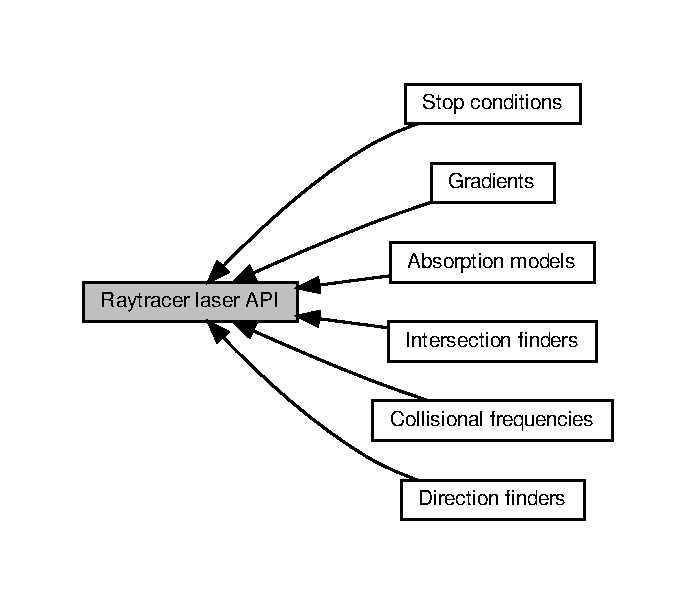
\includegraphics[width=334pt]{group__api}
\end{center}
\end{figure}
\subsection*{Modules}
\begin{DoxyCompactItemize}
\item 
\hyperlink{group__directionFinders}{Direction finders}
\begin{DoxyCompactList}\small\item\em Functions and functors to be used with \hyperlink{classraytracer_1_1Laser_a40fd2b112fb1de646861d7e93ac303e3}{Laser\+::generate\+Intersections()} as find\+Direction parameter. \end{DoxyCompactList}\item 
\hyperlink{group__intersectionFinders}{Intersection finders}
\begin{DoxyCompactList}\small\item\em Functions and functors to be used with \hyperlink{classraytracer_1_1Laser_a40fd2b112fb1de646861d7e93ac303e3}{Laser\+::generate\+Intersections()} as find\+Intersection parameter. \end{DoxyCompactList}\item 
\hyperlink{group__stopConditions}{Stop conditions}
\begin{DoxyCompactList}\small\item\em Functions and functors to be used with \hyperlink{classraytracer_1_1Laser_a40fd2b112fb1de646861d7e93ac303e3}{Laser\+::generate\+Intersections()} as stop\+Condition parameter. \end{DoxyCompactList}\item 
\hyperlink{group__gradients}{Gradients}
\begin{DoxyCompactList}\small\item\em \hyperlink{classraytracer_1_1Gradient}{Gradient} models to calculate gradient at given point in a \hyperlink{classraytracer_1_1MeshFunction}{Mesh\+Function}. \end{DoxyCompactList}\item 
\hyperlink{group__frequency}{Collisional frequencies}
\begin{DoxyCompactList}\small\item\em \hyperlink{classraytracer_1_1CollisionalFrequency}{Collisional\+Frequency} models to calculate collisional frequency. \end{DoxyCompactList}\item 
\hyperlink{group__absorption}{Absorption models}
\begin{DoxyCompactList}\small\item\em All possible \hyperlink{classraytracer_1_1AbsorptionModel}{Absorption\+Model} implementations are documented in this module. \end{DoxyCompactList}\end{DoxyCompactItemize}
\subsection*{Classes}
\begin{DoxyCompactItemize}
\item 
class \hyperlink{classraytracer_1_1Element}{raytracer\+::\+Element}
\begin{DoxyCompactList}\small\item\em Class representing a single polygonal element in mesh. \end{DoxyCompactList}\item 
class \hyperlink{classraytracer_1_1Face}{raytracer\+::\+Face}
\begin{DoxyCompactList}\small\item\em Class representing a polygonal face in mesh (edge in 2D, surface polygon face in 3D). \end{DoxyCompactList}\item 
struct \hyperlink{structraytracer_1_1PointOnFace}{raytracer\+::\+Point\+On\+Face}
\begin{DoxyCompactList}\small\item\em Structure representing a point on a face. \end{DoxyCompactList}\item 
struct \hyperlink{structraytracer_1_1DiscreteLine}{raytracer\+::\+Discrete\+Line}
\begin{DoxyCompactList}\small\item\em Structure representing a discretization of a distance. \end{DoxyCompactList}\item 
class \hyperlink{classraytracer_1_1Mesh}{raytracer\+::\+Mesh}
\begin{DoxyCompactList}\small\item\em Class representing a mesh (2D for now). \end{DoxyCompactList}\item 
class \hyperlink{classraytracer_1_1MeshFunction}{raytracer\+::\+Mesh\+Function}
\begin{DoxyCompactList}\small\item\em Abstract interface. \end{DoxyCompactList}\item 
class \hyperlink{classraytracer_1_1MfemMeshFunction}{raytracer\+::\+Mfem\+Mesh\+Function}
\begin{DoxyCompactList}\small\item\em Discrete function what has constant values at \hyperlink{classraytracer_1_1Mesh}{Mesh} elements. \end{DoxyCompactList}\item 
class \hyperlink{classraytracer_1_1Point}{raytracer\+::\+Point}
\begin{DoxyCompactList}\small\item\em Class representing a point A point is given by two coordinates x and y. \end{DoxyCompactList}\item 
class \hyperlink{classraytracer_1_1Vector}{raytracer\+::\+Vector}
\begin{DoxyCompactList}\small\item\em Class representing a physical vector. \end{DoxyCompactList}\item 
class \hyperlink{classraytracer_1_1AbsorptionController}{raytracer\+::\+Absorption\+Controller}
\begin{DoxyCompactList}\small\item\em Class aggregating all instances of \hyperlink{classraytracer_1_1AbsorptionModel}{Absorption\+Model} used to update absorbed\+Energy mesh\+Function. \end{DoxyCompactList}\item 
class \hyperlink{classraytracer_1_1Laser}{raytracer\+::\+Laser}
\begin{DoxyCompactList}\small\item\em Class representing a real physical laser. \end{DoxyCompactList}\end{DoxyCompactItemize}
\subsection*{Functions}
\begin{DoxyCompactItemize}
\item 
std\+::unique\+\_\+ptr$<$ mfem\+::\+Mesh $>$ \hyperlink{group__api_ga289222e1fc63a6e9126da5bbfa7b6a12}{raytracer\+::construct\+Rectangle\+Mesh} (\hyperlink{structraytracer_1_1DiscreteLine}{Discrete\+Line} sideA, \hyperlink{structraytracer_1_1DiscreteLine}{Discrete\+Line} sideB)
\begin{DoxyCompactList}\small\item\em Construct a mfem\+::\+Mesh given two discrete lines (the sides of the rectangle). \end{DoxyCompactList}\item 
const \hyperlink{classraytracer_1_1Vector}{Vector} \hyperlink{group__api_ga600238d4569fec2dd95c6fec3f4e8b30}{raytracer\+::operator-\/} (\hyperlink{classraytracer_1_1Point}{Point} A, \hyperlink{classraytracer_1_1Point}{Point} B)
\begin{DoxyCompactList}\small\item\em Two Points can be subtracted to get a \hyperlink{classraytracer_1_1Vector}{Vector}. \end{DoxyCompactList}\item 
const \hyperlink{classraytracer_1_1Point}{Point} \hyperlink{group__api_gaad5be472789d2f603e44e25b5d835708}{raytracer\+::operator+} (\hyperlink{classraytracer_1_1Point}{Point} A, \hyperlink{classraytracer_1_1Vector}{Vector} b)
\begin{DoxyCompactList}\small\item\em \hyperlink{classraytracer_1_1Vector}{Vector} and point can be added get another point. \end{DoxyCompactList}\item 
const \hyperlink{classraytracer_1_1Point}{Point} \hyperlink{group__api_ga4d268f6d854b65fc7b0c2b7331e233ae}{raytracer\+::operator+} (\hyperlink{classraytracer_1_1Vector}{Vector} b, \hyperlink{classraytracer_1_1Point}{Point} A)
\begin{DoxyCompactList}\small\item\em Convenience wrapper around A + b. \end{DoxyCompactList}\item 
const \hyperlink{classraytracer_1_1Vector}{Vector} \hyperlink{group__api_ga03236160eb138b0ee089b67a71d4978e}{raytracer\+::operator$\ast$} (double k, \hyperlink{classraytracer_1_1Vector}{Vector} a)
\begin{DoxyCompactList}\small\item\em \hyperlink{classraytracer_1_1Vector}{Vector} can be multiplied by number k$\ast$a. \end{DoxyCompactList}\item 
const \hyperlink{classraytracer_1_1Vector}{Vector} \hyperlink{group__api_ga299354d219d40b7431474c15b9718abb}{raytracer\+::operator$\ast$} (\hyperlink{classraytracer_1_1Vector}{Vector} a, double k)
\begin{DoxyCompactList}\small\item\em Convenience wrapper around k$\ast$a. \end{DoxyCompactList}\item 
double \hyperlink{group__api_gac6d4df29b0f3bc91c6744edb04582ef7}{raytracer\+::operator$\ast$} (\hyperlink{classraytracer_1_1Vector}{Vector} a, \hyperlink{classraytracer_1_1Vector}{Vector} b)
\begin{DoxyCompactList}\small\item\em his is the dot product of two vectors a, b \end{DoxyCompactList}\item 
const \hyperlink{classraytracer_1_1Vector}{Vector} \hyperlink{group__api_gaa2334c02fb14a238c09edd45c99e33fa}{raytracer\+::operator+} (\hyperlink{classraytracer_1_1Vector}{Vector} a, \hyperlink{classraytracer_1_1Vector}{Vector} b)
\begin{DoxyCompactList}\small\item\em Two vectors a, b can be added. \end{DoxyCompactList}\item 
const \hyperlink{classraytracer_1_1Vector}{Vector} \hyperlink{group__api_ga39d9dfe9600eef5b1e29f0baebc65e1c}{raytracer\+::operator-\/} (\hyperlink{classraytracer_1_1Vector}{Vector} a, \hyperlink{classraytracer_1_1Vector}{Vector} b)
\begin{DoxyCompactList}\small\item\em Two vectors a, b can be subtracted. \end{DoxyCompactList}\end{DoxyCompactItemize}


\subsection{Detailed Description}
This is the user A\+PI, refer to to this module or its submodules if you are a user of Raytracer. 

It is also highly recommended to use only abstractions from this A\+PI if you are not a developer of Raytracer. 

\subsection{Function Documentation}
\mbox{\Hypertarget{group__api_ga289222e1fc63a6e9126da5bbfa7b6a12}\label{group__api_ga289222e1fc63a6e9126da5bbfa7b6a12}} 
\index{Raytracer laser A\+PI@{Raytracer laser A\+PI}!construct\+Rectangle\+Mesh@{construct\+Rectangle\+Mesh}}
\index{construct\+Rectangle\+Mesh@{construct\+Rectangle\+Mesh}!Raytracer laser A\+PI@{Raytracer laser A\+PI}}
\subsubsection{\texorpdfstring{construct\+Rectangle\+Mesh()}{constructRectangleMesh()}}
{\footnotesize\ttfamily std\+::unique\+\_\+ptr$<$mfem\+::\+Mesh$>$ raytracer\+::construct\+Rectangle\+Mesh (\begin{DoxyParamCaption}\item[{\hyperlink{structraytracer_1_1DiscreteLine}{Discrete\+Line}}]{sideA,  }\item[{\hyperlink{structraytracer_1_1DiscreteLine}{Discrete\+Line}}]{sideB }\end{DoxyParamCaption})}



Construct a mfem\+::\+Mesh given two discrete lines (the sides of the rectangle). 

The mesh will be a rectangular equidistant grid beginning at (0, 0).


\begin{DoxyParams}{Parameters}
{\em sideA} & of the mesh \\
\hline
{\em sideB} & of the mesh \\
\hline
\end{DoxyParams}
\begin{DoxyReturn}{Returns}
the unique pointer to the mfem\+::\+Mesh 
\end{DoxyReturn}
\mbox{\Hypertarget{group__api_ga03236160eb138b0ee089b67a71d4978e}\label{group__api_ga03236160eb138b0ee089b67a71d4978e}} 
\index{Raytracer laser A\+PI@{Raytracer laser A\+PI}!operator$\ast$@{operator$\ast$}}
\index{operator$\ast$@{operator$\ast$}!Raytracer laser A\+PI@{Raytracer laser A\+PI}}
\subsubsection{\texorpdfstring{operator$\ast$()}{operator*()}\hspace{0.1cm}{\footnotesize\ttfamily [1/3]}}
{\footnotesize\ttfamily const \hyperlink{classraytracer_1_1Vector}{Vector} raytracer\+::operator$\ast$ (\begin{DoxyParamCaption}\item[{double}]{k,  }\item[{\hyperlink{classraytracer_1_1Vector}{Vector}}]{a }\end{DoxyParamCaption})}



\hyperlink{classraytracer_1_1Vector}{Vector} can be multiplied by number k$\ast$a. 


\begin{DoxyParams}{Parameters}
{\em k} & \\
\hline
{\em a} & \\
\hline
\end{DoxyParams}
\begin{DoxyReturn}{Returns}
scaled vector 
\end{DoxyReturn}
\mbox{\Hypertarget{group__api_ga299354d219d40b7431474c15b9718abb}\label{group__api_ga299354d219d40b7431474c15b9718abb}} 
\index{Raytracer laser A\+PI@{Raytracer laser A\+PI}!operator$\ast$@{operator$\ast$}}
\index{operator$\ast$@{operator$\ast$}!Raytracer laser A\+PI@{Raytracer laser A\+PI}}
\subsubsection{\texorpdfstring{operator$\ast$()}{operator*()}\hspace{0.1cm}{\footnotesize\ttfamily [2/3]}}
{\footnotesize\ttfamily const \hyperlink{classraytracer_1_1Vector}{Vector} raytracer\+::operator$\ast$ (\begin{DoxyParamCaption}\item[{\hyperlink{classraytracer_1_1Vector}{Vector}}]{a,  }\item[{double}]{k }\end{DoxyParamCaption})}



Convenience wrapper around k$\ast$a. 


\begin{DoxyParams}{Parameters}
{\em a} & \\
\hline
{\em k} & \\
\hline
\end{DoxyParams}
\begin{DoxyReturn}{Returns}

\end{DoxyReturn}
\mbox{\Hypertarget{group__api_gac6d4df29b0f3bc91c6744edb04582ef7}\label{group__api_gac6d4df29b0f3bc91c6744edb04582ef7}} 
\index{Raytracer laser A\+PI@{Raytracer laser A\+PI}!operator$\ast$@{operator$\ast$}}
\index{operator$\ast$@{operator$\ast$}!Raytracer laser A\+PI@{Raytracer laser A\+PI}}
\subsubsection{\texorpdfstring{operator$\ast$()}{operator*()}\hspace{0.1cm}{\footnotesize\ttfamily [3/3]}}
{\footnotesize\ttfamily double raytracer\+::operator$\ast$ (\begin{DoxyParamCaption}\item[{\hyperlink{classraytracer_1_1Vector}{Vector}}]{a,  }\item[{\hyperlink{classraytracer_1_1Vector}{Vector}}]{b }\end{DoxyParamCaption})}



his is the dot product of two vectors a, b 


\begin{DoxyParams}{Parameters}
{\em a} & \\
\hline
{\em b} & \\
\hline
\end{DoxyParams}
\begin{DoxyReturn}{Returns}
dot product 
\end{DoxyReturn}
\mbox{\Hypertarget{group__api_gaad5be472789d2f603e44e25b5d835708}\label{group__api_gaad5be472789d2f603e44e25b5d835708}} 
\index{Raytracer laser A\+PI@{Raytracer laser A\+PI}!operator+@{operator+}}
\index{operator+@{operator+}!Raytracer laser A\+PI@{Raytracer laser A\+PI}}
\subsubsection{\texorpdfstring{operator+()}{operator+()}\hspace{0.1cm}{\footnotesize\ttfamily [1/3]}}
{\footnotesize\ttfamily const \hyperlink{classraytracer_1_1Point}{Point} raytracer\+::operator+ (\begin{DoxyParamCaption}\item[{\hyperlink{classraytracer_1_1Point}{Point}}]{A,  }\item[{\hyperlink{classraytracer_1_1Vector}{Vector}}]{b }\end{DoxyParamCaption})}



\hyperlink{classraytracer_1_1Vector}{Vector} and point can be added get another point. 


\begin{DoxyParams}{Parameters}
{\em A} & point \\
\hline
{\em b} & vector \\
\hline
\end{DoxyParams}
\begin{DoxyReturn}{Returns}
\hyperlink{classraytracer_1_1Point}{Point} given by vector added to point A 
\end{DoxyReturn}
\mbox{\Hypertarget{group__api_ga4d268f6d854b65fc7b0c2b7331e233ae}\label{group__api_ga4d268f6d854b65fc7b0c2b7331e233ae}} 
\index{Raytracer laser A\+PI@{Raytracer laser A\+PI}!operator+@{operator+}}
\index{operator+@{operator+}!Raytracer laser A\+PI@{Raytracer laser A\+PI}}
\subsubsection{\texorpdfstring{operator+()}{operator+()}\hspace{0.1cm}{\footnotesize\ttfamily [2/3]}}
{\footnotesize\ttfamily const \hyperlink{classraytracer_1_1Point}{Point} raytracer\+::operator+ (\begin{DoxyParamCaption}\item[{\hyperlink{classraytracer_1_1Vector}{Vector}}]{b,  }\item[{\hyperlink{classraytracer_1_1Point}{Point}}]{A }\end{DoxyParamCaption})}



Convenience wrapper around A + b. 


\begin{DoxyParams}{Parameters}
{\em b} & \\
\hline
{\em A} & \\
\hline
\end{DoxyParams}
\begin{DoxyReturn}{Returns}

\end{DoxyReturn}
\mbox{\Hypertarget{group__api_gaa2334c02fb14a238c09edd45c99e33fa}\label{group__api_gaa2334c02fb14a238c09edd45c99e33fa}} 
\index{Raytracer laser A\+PI@{Raytracer laser A\+PI}!operator+@{operator+}}
\index{operator+@{operator+}!Raytracer laser A\+PI@{Raytracer laser A\+PI}}
\subsubsection{\texorpdfstring{operator+()}{operator+()}\hspace{0.1cm}{\footnotesize\ttfamily [3/3]}}
{\footnotesize\ttfamily const \hyperlink{classraytracer_1_1Vector}{Vector} raytracer\+::operator+ (\begin{DoxyParamCaption}\item[{\hyperlink{classraytracer_1_1Vector}{Vector}}]{a,  }\item[{\hyperlink{classraytracer_1_1Vector}{Vector}}]{b }\end{DoxyParamCaption})}



Two vectors a, b can be added. 


\begin{DoxyParams}{Parameters}
{\em a} & \\
\hline
{\em b} & \\
\hline
\end{DoxyParams}
\begin{DoxyReturn}{Returns}

\end{DoxyReturn}
\mbox{\Hypertarget{group__api_ga600238d4569fec2dd95c6fec3f4e8b30}\label{group__api_ga600238d4569fec2dd95c6fec3f4e8b30}} 
\index{Raytracer laser A\+PI@{Raytracer laser A\+PI}!operator-\/@{operator-\/}}
\index{operator-\/@{operator-\/}!Raytracer laser A\+PI@{Raytracer laser A\+PI}}
\subsubsection{\texorpdfstring{operator-\/()}{operator-()}\hspace{0.1cm}{\footnotesize\ttfamily [1/2]}}
{\footnotesize\ttfamily const \hyperlink{classraytracer_1_1Vector}{Vector} raytracer\+::operator-\/ (\begin{DoxyParamCaption}\item[{\hyperlink{classraytracer_1_1Point}{Point}}]{A,  }\item[{\hyperlink{classraytracer_1_1Point}{Point}}]{B }\end{DoxyParamCaption})}



Two Points can be subtracted to get a \hyperlink{classraytracer_1_1Vector}{Vector}. 


\begin{DoxyParams}{Parameters}
{\em A} & point \\
\hline
{\em B} & point \\
\hline
\end{DoxyParams}
\begin{DoxyReturn}{Returns}
vector given by points difference 
\end{DoxyReturn}
\mbox{\Hypertarget{group__api_ga39d9dfe9600eef5b1e29f0baebc65e1c}\label{group__api_ga39d9dfe9600eef5b1e29f0baebc65e1c}} 
\index{Raytracer laser A\+PI@{Raytracer laser A\+PI}!operator-\/@{operator-\/}}
\index{operator-\/@{operator-\/}!Raytracer laser A\+PI@{Raytracer laser A\+PI}}
\subsubsection{\texorpdfstring{operator-\/()}{operator-()}\hspace{0.1cm}{\footnotesize\ttfamily [2/2]}}
{\footnotesize\ttfamily const \hyperlink{classraytracer_1_1Vector}{Vector} raytracer\+::operator-\/ (\begin{DoxyParamCaption}\item[{\hyperlink{classraytracer_1_1Vector}{Vector}}]{a,  }\item[{\hyperlink{classraytracer_1_1Vector}{Vector}}]{b }\end{DoxyParamCaption})}



Two vectors a, b can be subtracted. 


\begin{DoxyParams}{Parameters}
{\em a} & \\
\hline
{\em b} & \\
\hline
\end{DoxyParams}
\begin{DoxyReturn}{Returns}

\end{DoxyReturn}

\hypertarget{group__directionFinders}{}\section{Direction finders}
\label{group__directionFinders}\index{Direction finders@{Direction finders}}


Functions and functors to be used with \hyperlink{classraytracer_1_1Laser_a40fd2b112fb1de646861d7e93ac303e3}{Laser\+::generate\+Intersections()} as find\+Direction parameter.  


Collaboration diagram for Direction finders\+:
\nopagebreak
\begin{figure}[H]
\begin{center}
\leavevmode
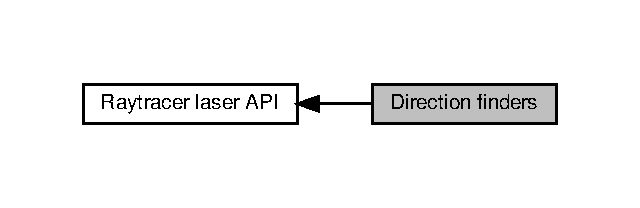
\includegraphics[width=307pt]{group__directionFinders}
\end{center}
\end{figure}
\subsection*{Classes}
\begin{DoxyCompactItemize}
\item 
struct \hyperlink{structraytracer_1_1ContinueStraight}{raytracer\+::\+Continue\+Straight}
\begin{DoxyCompactList}\small\item\em Functor that returns always the previous\+Direction. \end{DoxyCompactList}\item 
struct \hyperlink{structraytracer_1_1SnellsLaw}{raytracer\+::\+Snells\+Law}
\begin{DoxyCompactList}\small\item\em Functor that finds new direction base on the Snells\textquotesingle{}s law. \end{DoxyCompactList}\end{DoxyCompactItemize}


\subsection{Detailed Description}
Functions and functors to be used with \hyperlink{classraytracer_1_1Laser_a40fd2b112fb1de646861d7e93ac303e3}{Laser\+::generate\+Intersections()} as find\+Direction parameter. 


\hypertarget{group__intersectionFinders}{}\section{Intersection finders}
\label{group__intersectionFinders}\index{Intersection finders@{Intersection finders}}


Functions and functors to be used with \hyperlink{classraytracer_1_1Laser_a40fd2b112fb1de646861d7e93ac303e3}{Laser\+::generate\+Intersections()} as find\+Intersection parameter.  


Collaboration diagram for Intersection finders\+:
\nopagebreak
\begin{figure}[H]
\begin{center}
\leavevmode
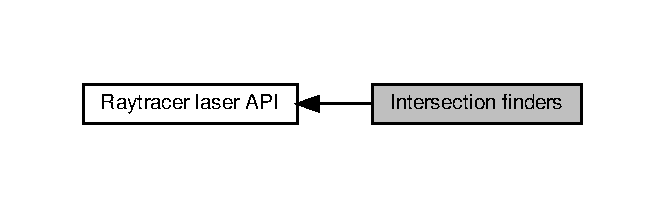
\includegraphics[width=319pt]{group__intersectionFinders}
\end{center}
\end{figure}
\subsection*{Functions}
\begin{DoxyCompactItemize}
\item 
\hyperlink{structraytracer_1_1PointOnFace}{Point\+On\+Face} \hyperlink{group__intersectionFinders_ga88bd3438a657bdf333afdd59cd675798}{raytracer\+::intersect\+Straight} (const \hyperlink{structraytracer_1_1PointOnFace}{Point\+On\+Face} \&entry\+Point\+On\+Face, const \hyperlink{classraytracer_1_1Vector}{Vector} \&entry\+Direction, const \hyperlink{classraytracer_1_1Element}{Element} \&element, const \hyperlink{classraytracer_1_1LaserRay}{Laser\+Ray} \&)
\begin{DoxyCompactList}\small\item\em Function to be used in \hyperlink{classraytracer_1_1Laser_a40fd2b112fb1de646861d7e93ac303e3}{Laser\+::generate\+Intersections()} as find\+Intersection. \end{DoxyCompactList}\end{DoxyCompactItemize}


\subsection{Detailed Description}
Functions and functors to be used with \hyperlink{classraytracer_1_1Laser_a40fd2b112fb1de646861d7e93ac303e3}{Laser\+::generate\+Intersections()} as find\+Intersection parameter. 



\subsection{Function Documentation}
\mbox{\Hypertarget{group__intersectionFinders_ga88bd3438a657bdf333afdd59cd675798}\label{group__intersectionFinders_ga88bd3438a657bdf333afdd59cd675798}} 
\index{Intersection finders@{Intersection finders}!intersect\+Straight@{intersect\+Straight}}
\index{intersect\+Straight@{intersect\+Straight}!Intersection finders@{Intersection finders}}
\subsubsection{\texorpdfstring{intersect\+Straight()}{intersectStraight()}}
{\footnotesize\ttfamily \hyperlink{structraytracer_1_1PointOnFace}{Point\+On\+Face} raytracer\+::intersect\+Straight (\begin{DoxyParamCaption}\item[{const \hyperlink{structraytracer_1_1PointOnFace}{Point\+On\+Face} \&}]{entry\+Point\+On\+Face,  }\item[{const \hyperlink{classraytracer_1_1Vector}{Vector} \&}]{entry\+Direction,  }\item[{const \hyperlink{classraytracer_1_1Element}{Element} \&}]{element,  }\item[{const \hyperlink{classraytracer_1_1LaserRay}{Laser\+Ray} \&}]{ }\end{DoxyParamCaption})}



Function to be used in \hyperlink{classraytracer_1_1Laser_a40fd2b112fb1de646861d7e93ac303e3}{Laser\+::generate\+Intersections()} as find\+Intersection. 

It intersects the element in straight line. 
\begin{DoxyParams}{Parameters}
{\em entry\+Point\+On\+Face} & \\
\hline
{\em entry\+Direction} & \\
\hline
{\em element} & \\
\hline
\end{DoxyParams}
\begin{DoxyReturn}{Returns}
intersecting point in straight line from entry\+Point\+On\+Face 
\end{DoxyReturn}

\hypertarget{group__stopConditions}{}\section{Stop conditions}
\label{group__stopConditions}\index{Stop conditions@{Stop conditions}}


Functions and functors to be used with \hyperlink{classraytracer_1_1Laser_a40fd2b112fb1de646861d7e93ac303e3}{Laser\+::generate\+Intersections()} as stop\+Condition parameter.  


Collaboration diagram for Stop conditions\+:
\nopagebreak
\begin{figure}[H]
\begin{center}
\leavevmode
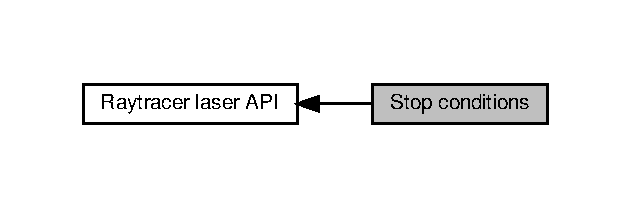
\includegraphics[width=303pt]{group__stopConditions}
\end{center}
\end{figure}
\subsection*{Classes}
\begin{DoxyCompactItemize}
\item 
struct \hyperlink{structraytracer_1_1StopAtCritical}{raytracer\+::\+Stop\+At\+Critical}
\begin{DoxyCompactList}\small\item\em Functor for ray propagation termination based on critical density expected to used with lase\+Ray intersection finding procedure. \end{DoxyCompactList}\item 
struct \hyperlink{structraytracer_1_1DontStop}{raytracer\+::\+Dont\+Stop}
\begin{DoxyCompactList}\small\item\em Functor for ray propagation that returns false in any case. \end{DoxyCompactList}\end{DoxyCompactItemize}


\subsection{Detailed Description}
Functions and functors to be used with \hyperlink{classraytracer_1_1Laser_a40fd2b112fb1de646861d7e93ac303e3}{Laser\+::generate\+Intersections()} as stop\+Condition parameter. 


\hypertarget{group__gradients}{}\section{Gradients}
\label{group__gradients}\index{Gradients@{Gradients}}


\hyperlink{classraytracer_1_1Gradient}{Gradient} models to calculate gradient at given point in a \hyperlink{classraytracer_1_1MeshFunction}{Mesh\+Function}.  


Collaboration diagram for Gradients\+:
\nopagebreak
\begin{figure}[H]
\begin{center}
\leavevmode
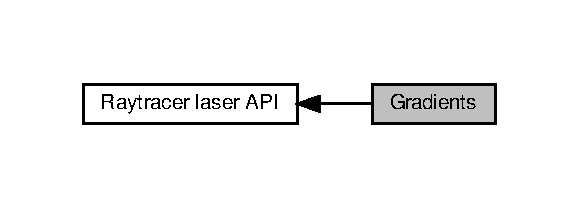
\includegraphics[width=278pt]{group__gradients}
\end{center}
\end{figure}
\subsection*{Classes}
\begin{DoxyCompactItemize}
\item 
class \hyperlink{classraytracer_1_1Gradient}{raytracer\+::\+Gradient}
\begin{DoxyCompactList}\small\item\em Abstract interface to provide a Gradient\+Calculator. \end{DoxyCompactList}\item 
class \hyperlink{classraytracer_1_1ConstantGradient}{raytracer\+::\+Constant\+Gradient}
\begin{DoxyCompactList}\small\item\em Gradient\+Calculator that returns a constant \hyperlink{classraytracer_1_1Vector}{Vector} no matter what. \end{DoxyCompactList}\item 
class \hyperlink{classraytracer_1_1H1Gradient}{raytracer\+::\+H1\+Gradient}
\begin{DoxyCompactList}\small\item\em Gradient\+Calculator that stores a density grid function defined in H1 space obtained from function given if L2. \end{DoxyCompactList}\item 
class \hyperlink{classraytracer_1_1StepGradient}{raytracer\+::\+Step\+Gradient}
\begin{DoxyCompactList}\small\item\em Gradient\+Calculator that returns the normal to the face as \hyperlink{classraytracer_1_1Gradient}{Gradient}. \end{DoxyCompactList}\end{DoxyCompactItemize}


\subsection{Detailed Description}
\hyperlink{classraytracer_1_1Gradient}{Gradient} models to calculate gradient at given point in a \hyperlink{classraytracer_1_1MeshFunction}{Mesh\+Function}. 


\hypertarget{group__frequency}{}\section{Collisional frequencies}
\label{group__frequency}\index{Collisional frequencies@{Collisional frequencies}}


\hyperlink{classraytracer_1_1CollisionalFrequency}{Collisional\+Frequency} models to calculate collisional frequency.  


Collaboration diagram for Collisional frequencies\+:
\nopagebreak
\begin{figure}[H]
\begin{center}
\leavevmode
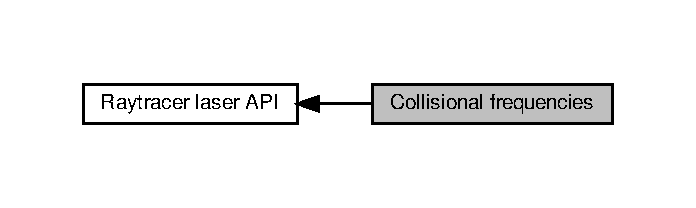
\includegraphics[width=334pt]{group__frequency}
\end{center}
\end{figure}
\subsection*{Classes}
\begin{DoxyCompactItemize}
\item 
class \hyperlink{classraytracer_1_1CollisionalFrequency}{raytracer\+::\+Collisional\+Frequency}
\begin{DoxyCompactList}\small\item\em Abstract interface. \end{DoxyCompactList}\item 
class \hyperlink{classraytracer_1_1SpitzerFrequency}{raytracer\+::\+Spitzer\+Frequency}
\begin{DoxyCompactList}\small\item\em Class representing a Spitzer-\/\+Harm frequency calculator. \end{DoxyCompactList}\end{DoxyCompactItemize}


\subsection{Detailed Description}
\hyperlink{classraytracer_1_1CollisionalFrequency}{Collisional\+Frequency} models to calculate collisional frequency. 


\hypertarget{group__absorption}{}\section{Absorption models}
\label{group__absorption}\index{Absorption models@{Absorption models}}


All possible \hyperlink{classraytracer_1_1AbsorptionModel}{Absorption\+Model} implementations are documented in this module.  


Collaboration diagram for Absorption models\+:
\nopagebreak
\begin{figure}[H]
\begin{center}
\leavevmode
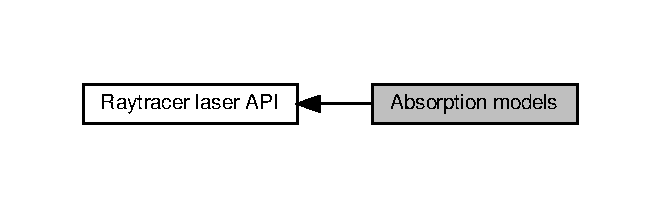
\includegraphics[width=317pt]{group__absorption}
\end{center}
\end{figure}
\subsection*{Classes}
\begin{DoxyCompactItemize}
\item 
class \hyperlink{classraytracer_1_1AbsorptionModel}{raytracer\+::\+Absorption\+Model}
\begin{DoxyCompactList}\small\item\em Abstract interface, to obey this get\+Energy\+Change must be implemented. \end{DoxyCompactList}\item 
struct \hyperlink{structraytracer_1_1Bremsstrahlung}{raytracer\+::\+Bremsstrahlung}
\begin{DoxyCompactList}\small\item\em Absorption model of energy exchange due to bremsstrahlung. \end{DoxyCompactList}\end{DoxyCompactItemize}


\subsection{Detailed Description}
All possible \hyperlink{classraytracer_1_1AbsorptionModel}{Absorption\+Model} implementations are documented in this module. 


\chapter{Namespace Documentation}
\hypertarget{namespaceraytracer}{}\section{raytracer Namespace Reference}
\label{namespaceraytracer}\index{raytracer@{raytracer}}


Namespace of the whole library.  


\subsection*{Namespaces}
\begin{DoxyCompactItemize}
\item 
 \hyperlink{namespaceraytracer_1_1geometry}{geometry}
\begin{DoxyCompactList}\small\item\em Namespace encapsulating all the abstractions related to geometry. \end{DoxyCompactList}\end{DoxyCompactItemize}


\subsection{Detailed Description}
Namespace of the whole library. 
\hypertarget{namespaceraytracer_1_1constants}{}\section{raytracer\+:\+:constants Namespace Reference}
\label{namespaceraytracer_1_1constants}\index{raytracer\+::constants@{raytracer\+::constants}}


Basic physics constants in cgs units.  


\subsection*{Variables}
\begin{DoxyCompactItemize}
\item 
\mbox{\Hypertarget{namespaceraytracer_1_1constants_a57321c1a2dc6a7a5362032408479da32}\label{namespaceraytracer_1_1constants_a57321c1a2dc6a7a5362032408479da32}} 
constexpr double \hyperlink{namespaceraytracer_1_1constants_a57321c1a2dc6a7a5362032408479da32}{electron\+\_\+charge} = 4.\+8032068e-\/10
\begin{DoxyCompactList}\small\item\em Electron charge in cgs. \end{DoxyCompactList}\item 
\mbox{\Hypertarget{namespaceraytracer_1_1constants_a8718033b4f3abf19d6eb32078ae24efa}\label{namespaceraytracer_1_1constants_a8718033b4f3abf19d6eb32078ae24efa}} 
constexpr double \hyperlink{namespaceraytracer_1_1constants_a8718033b4f3abf19d6eb32078ae24efa}{electron\+\_\+mass} = 9.\+1093897e-\/28
\begin{DoxyCompactList}\small\item\em Electron mass in cgs. \end{DoxyCompactList}\item 
\mbox{\Hypertarget{namespaceraytracer_1_1constants_a0325b8d091645d6938691f865bfb9a5c}\label{namespaceraytracer_1_1constants_a0325b8d091645d6938691f865bfb9a5c}} 
constexpr double \hyperlink{namespaceraytracer_1_1constants_a0325b8d091645d6938691f865bfb9a5c}{speed\+\_\+of\+\_\+light} = 2.\+99792458e10
\begin{DoxyCompactList}\small\item\em Speed of light in cgs. \end{DoxyCompactList}\item 
\mbox{\Hypertarget{namespaceraytracer_1_1constants_aa74c1423a0ee9b86e821050da5a2c23d}\label{namespaceraytracer_1_1constants_aa74c1423a0ee9b86e821050da5a2c23d}} 
constexpr double \hyperlink{namespaceraytracer_1_1constants_aa74c1423a0ee9b86e821050da5a2c23d}{proton\+\_\+mass} = 1.\+6605e-\/24
\begin{DoxyCompactList}\small\item\em Proton mass in cgs. \end{DoxyCompactList}\item 
\mbox{\Hypertarget{namespaceraytracer_1_1constants_ac2c1dccc26c3700a9b934e11245ee79f}\label{namespaceraytracer_1_1constants_ac2c1dccc26c3700a9b934e11245ee79f}} 
constexpr double \hyperlink{namespaceraytracer_1_1constants_ac2c1dccc26c3700a9b934e11245ee79f}{boltzmann\+\_\+constant} = 1.\+602115e-\/12
\begin{DoxyCompactList}\small\item\em Boltzmann constant in cgs. \end{DoxyCompactList}\item 
\mbox{\Hypertarget{namespaceraytracer_1_1constants_a57166090154a8f6df45d2f6dd3fbb3b9}\label{namespaceraytracer_1_1constants_a57166090154a8f6df45d2f6dd3fbb3b9}} 
constexpr double \hyperlink{namespaceraytracer_1_1constants_a57166090154a8f6df45d2f6dd3fbb3b9}{planck\+\_\+constant} = 6.\+626068760e-\/27
\begin{DoxyCompactList}\small\item\em Planck constant in cgs. \end{DoxyCompactList}\item 
\mbox{\Hypertarget{namespaceraytracer_1_1constants_a3bc79d50e2cd8d00e0a699fe06f6a52e}\label{namespaceraytracer_1_1constants_a3bc79d50e2cd8d00e0a699fe06f6a52e}} 
constexpr double \hyperlink{namespaceraytracer_1_1constants_a3bc79d50e2cd8d00e0a699fe06f6a52e}{reduced\+\_\+planck\+\_\+constant} = 1.\+054571596e-\/27
\begin{DoxyCompactList}\small\item\em Reduced Planck constant in cgs. \end{DoxyCompactList}\item 
\mbox{\Hypertarget{namespaceraytracer_1_1constants_a93db781cf79ad352e206eaf666719fbd}\label{namespaceraytracer_1_1constants_a93db781cf79ad352e206eaf666719fbd}} 
constexpr double \hyperlink{namespaceraytracer_1_1constants_a93db781cf79ad352e206eaf666719fbd}{atomic\+\_\+mass\+\_\+unit} = 1.\+6605e-\/24
\begin{DoxyCompactList}\small\item\em Atomic mass unit in cgs. \end{DoxyCompactList}\end{DoxyCompactItemize}


\subsection{Detailed Description}
Basic physics constants in cgs units. 
\chapter{Class Documentation}
\hypertarget{classraytracer_1_1AbsorptionController}{}\section{raytracer\+:\+:Absorption\+Controller Class Reference}
\label{classraytracer_1_1AbsorptionController}\index{raytracer\+::\+Absorption\+Controller@{raytracer\+::\+Absorption\+Controller}}


Class aggregating all instances of \hyperlink{classraytracer_1_1AbsorptionModel}{Absorption\+Model} used to update absorbed\+Energy mesh\+Function.  




{\ttfamily \#include $<$Absorption.\+h$>$}

\subsection*{Public Member Functions}
\begin{DoxyCompactItemize}
\item 
void \hyperlink{classraytracer_1_1AbsorptionController_a4bde685a4fe1a5adc873e1483d91e2ae}{add\+Model} (const \hyperlink{classraytracer_1_1AbsorptionModel}{Absorption\+Model} $\ast$model)
\begin{DoxyCompactList}\small\item\em Add an \hyperlink{classraytracer_1_1AbsorptionModel}{Absorption\+Model} that will be used when calling \hyperlink{classraytracer_1_1AbsorptionController_a5190d4b54293231350d30f3bf3acc59a}{absorb()}. \end{DoxyCompactList}\item 
void \hyperlink{classraytracer_1_1AbsorptionController_a5190d4b54293231350d30f3bf3acc59a}{absorb} (const \hyperlink{classraytracer_1_1Laser}{Laser} \&laser, \hyperlink{classraytracer_1_1MeshFunction}{Mesh\+Function} \&absorbed\+Energy)
\begin{DoxyCompactList}\small\item\em Add energy values based on \hyperlink{classraytracer_1_1AbsorptionModel}{Absorption\+Model} applied on the \hyperlink{classraytracer_1_1Laser}{Laser} to the absorbed\+Energy \hyperlink{classraytracer_1_1MeshFunction}{Mesh\+Function}. \end{DoxyCompactList}\end{DoxyCompactItemize}


\subsection{Detailed Description}
Class aggregating all instances of \hyperlink{classraytracer_1_1AbsorptionModel}{Absorption\+Model} used to update absorbed\+Energy mesh\+Function. 

\subsection{Member Function Documentation}
\mbox{\Hypertarget{classraytracer_1_1AbsorptionController_a5190d4b54293231350d30f3bf3acc59a}\label{classraytracer_1_1AbsorptionController_a5190d4b54293231350d30f3bf3acc59a}} 
\index{raytracer\+::\+Absorption\+Controller@{raytracer\+::\+Absorption\+Controller}!absorb@{absorb}}
\index{absorb@{absorb}!raytracer\+::\+Absorption\+Controller@{raytracer\+::\+Absorption\+Controller}}
\subsubsection{\texorpdfstring{absorb()}{absorb()}}
{\footnotesize\ttfamily void raytracer\+::\+Absorption\+Controller\+::absorb (\begin{DoxyParamCaption}\item[{const \hyperlink{classraytracer_1_1Laser}{Laser} \&}]{laser,  }\item[{\hyperlink{classraytracer_1_1MeshFunction}{Mesh\+Function} \&}]{absorbed\+Energy }\end{DoxyParamCaption})}



Add energy values based on \hyperlink{classraytracer_1_1AbsorptionModel}{Absorption\+Model} applied on the \hyperlink{classraytracer_1_1Laser}{Laser} to the absorbed\+Energy \hyperlink{classraytracer_1_1MeshFunction}{Mesh\+Function}. 

\begin{DoxyWarning}{Warning}
For this to work properly, \hyperlink{classraytracer_1_1Laser_a40fd2b112fb1de646861d7e93ac303e3}{Laser\+::generate\+Intersections()} must be called first. 
\end{DoxyWarning}

\begin{DoxyParams}{Parameters}
{\em laser} & \\
\hline
{\em absorbed\+Energy} & \\
\hline
\end{DoxyParams}
\mbox{\Hypertarget{classraytracer_1_1AbsorptionController_a4bde685a4fe1a5adc873e1483d91e2ae}\label{classraytracer_1_1AbsorptionController_a4bde685a4fe1a5adc873e1483d91e2ae}} 
\index{raytracer\+::\+Absorption\+Controller@{raytracer\+::\+Absorption\+Controller}!add\+Model@{add\+Model}}
\index{add\+Model@{add\+Model}!raytracer\+::\+Absorption\+Controller@{raytracer\+::\+Absorption\+Controller}}
\subsubsection{\texorpdfstring{add\+Model()}{addModel()}}
{\footnotesize\ttfamily void raytracer\+::\+Absorption\+Controller\+::add\+Model (\begin{DoxyParamCaption}\item[{const \hyperlink{classraytracer_1_1AbsorptionModel}{Absorption\+Model} $\ast$}]{model }\end{DoxyParamCaption})}



Add an \hyperlink{classraytracer_1_1AbsorptionModel}{Absorption\+Model} that will be used when calling \hyperlink{classraytracer_1_1AbsorptionController_a5190d4b54293231350d30f3bf3acc59a}{absorb()}. 


\begin{DoxyParams}{Parameters}
{\em model} & \\
\hline
\end{DoxyParams}


The documentation for this class was generated from the following file\+:\begin{DoxyCompactItemize}
\item 
/home/martin/\+C\+Lion\+Projects/raytracer/include/raytracer/physics/Absorption.\+h\end{DoxyCompactItemize}

\hypertarget{classraytracer_1_1AbsorptionModel}{}\section{raytracer\+:\+:Absorption\+Model Class Reference}
\label{classraytracer_1_1AbsorptionModel}\index{raytracer\+::\+Absorption\+Model@{raytracer\+::\+Absorption\+Model}}


Abstract interface, to obey this get\+Energy\+Change must be implemented.  




{\ttfamily \#include $<$Absorption.\+h$>$}



Inheritance diagram for raytracer\+:\+:Absorption\+Model\+:
\nopagebreak
\begin{figure}[H]
\begin{center}
\leavevmode
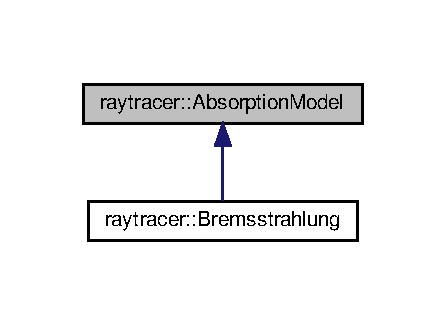
\includegraphics[width=214pt]{classraytracer_1_1AbsorptionModel__inherit__graph}
\end{center}
\end{figure}
\subsection*{Public Member Functions}
\begin{DoxyCompactItemize}
\item 
virtual \hyperlink{structraytracer_1_1Energy}{Energy} \hyperlink{classraytracer_1_1AbsorptionModel_a71abeb7d444a7c3cf56dc542657cc7d2}{get\+Energy\+Change} (const \hyperlink{structraytracer_1_1Intersection}{Intersection} \&previous\+Intersection, const \hyperlink{structraytracer_1_1Intersection}{Intersection} \&current\+Intersection, const \hyperlink{structraytracer_1_1Energy}{Energy} \&current\+Energy, const \hyperlink{classraytracer_1_1LaserRay}{Laser\+Ray} \&laser\+Ray) const =0
\begin{DoxyCompactList}\small\item\em Based on intersections of tray with the element, calculate how much energy was absorbed in this specific element. \end{DoxyCompactList}\end{DoxyCompactItemize}


\subsection{Detailed Description}
Abstract interface, to obey this get\+Energy\+Change must be implemented. 

\subsection{Member Function Documentation}
\mbox{\Hypertarget{classraytracer_1_1AbsorptionModel_a71abeb7d444a7c3cf56dc542657cc7d2}\label{classraytracer_1_1AbsorptionModel_a71abeb7d444a7c3cf56dc542657cc7d2}} 
\index{raytracer\+::\+Absorption\+Model@{raytracer\+::\+Absorption\+Model}!get\+Energy\+Change@{get\+Energy\+Change}}
\index{get\+Energy\+Change@{get\+Energy\+Change}!raytracer\+::\+Absorption\+Model@{raytracer\+::\+Absorption\+Model}}
\subsubsection{\texorpdfstring{get\+Energy\+Change()}{getEnergyChange()}}
{\footnotesize\ttfamily virtual \hyperlink{structraytracer_1_1Energy}{Energy} raytracer\+::\+Absorption\+Model\+::get\+Energy\+Change (\begin{DoxyParamCaption}\item[{const \hyperlink{structraytracer_1_1Intersection}{Intersection} \&}]{previous\+Intersection,  }\item[{const \hyperlink{structraytracer_1_1Intersection}{Intersection} \&}]{current\+Intersection,  }\item[{const \hyperlink{structraytracer_1_1Energy}{Energy} \&}]{current\+Energy,  }\item[{const \hyperlink{classraytracer_1_1LaserRay}{Laser\+Ray} \&}]{laser\+Ray }\end{DoxyParamCaption}) const\hspace{0.3cm}{\ttfamily [pure virtual]}}



Based on intersections of tray with the element, calculate how much energy was absorbed in this specific element. 


\begin{DoxyParams}{Parameters}
{\em previous\+Intersection} & \\
\hline
{\em current\+Intersection} & \\
\hline
{\em current\+Energy} & \\
\hline
{\em laser\+Ray} & \\
\hline
\end{DoxyParams}
\begin{DoxyReturn}{Returns}

\end{DoxyReturn}


Implemented in \hyperlink{structraytracer_1_1Bremsstrahlung_a510d57af7c09bb24d786afab8086b748}{raytracer\+::\+Bremsstrahlung}.



The documentation for this class was generated from the following file\+:\begin{DoxyCompactItemize}
\item 
/home/martin/\+C\+Lion\+Projects/raytracer/include/raytracer/physics/Absorption.\+h\end{DoxyCompactItemize}

\hypertarget{structraytracer_1_1Bremsstrahlung}{}\section{raytracer\+:\+:Bremsstrahlung Struct Reference}
\label{structraytracer_1_1Bremsstrahlung}\index{raytracer\+::\+Bremsstrahlung@{raytracer\+::\+Bremsstrahlung}}


Absorption model of energy exchange due to bremsstrahlung.  




{\ttfamily \#include $<$Absorption.\+h$>$}



Inheritance diagram for raytracer\+:\+:Bremsstrahlung\+:
\nopagebreak
\begin{figure}[H]
\begin{center}
\leavevmode
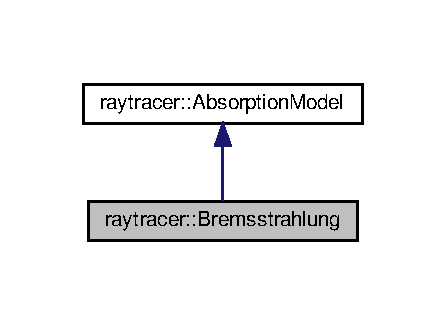
\includegraphics[width=214pt]{structraytracer_1_1Bremsstrahlung__inherit__graph}
\end{center}
\end{figure}


Collaboration diagram for raytracer\+:\+:Bremsstrahlung\+:
\nopagebreak
\begin{figure}[H]
\begin{center}
\leavevmode
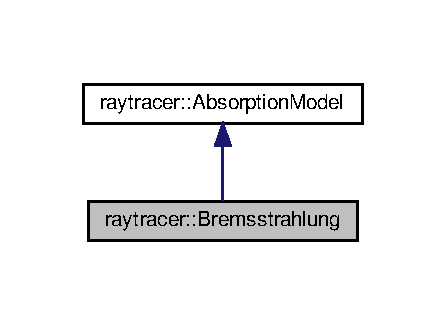
\includegraphics[width=214pt]{structraytracer_1_1Bremsstrahlung__coll__graph}
\end{center}
\end{figure}
\subsection*{Public Member Functions}
\begin{DoxyCompactItemize}
\item 
\hyperlink{structraytracer_1_1Bremsstrahlung_aa987a459be2174c29a33a2f8a5845c95}{Bremsstrahlung} (const \hyperlink{classraytracer_1_1MeshFunction}{Mesh\+Function} \&density, const \hyperlink{classraytracer_1_1MeshFunction}{Mesh\+Function} \&temperature, const \hyperlink{classraytracer_1_1MeshFunction}{Mesh\+Function} \&ionization, const \hyperlink{classraytracer_1_1CollisionalFrequency}{Collisional\+Frequency} \&collisional\+Frequency)
\begin{DoxyCompactList}\small\item\em To be able to model bremsstrahlung, \hyperlink{classraytracer_1_1MeshFunction}{Mesh\+Function} density, temperature, ionization must be provided. \end{DoxyCompactList}\item 
\hyperlink{structraytracer_1_1Energy}{Energy} \hyperlink{structraytracer_1_1Bremsstrahlung_a510d57af7c09bb24d786afab8086b748}{get\+Energy\+Change} (const \hyperlink{structraytracer_1_1Intersection}{Intersection} \&previous\+Intersection, const \hyperlink{structraytracer_1_1Intersection}{Intersection} \&current\+Intersection, const \hyperlink{structraytracer_1_1Energy}{Energy} \&current\+Energy, const \hyperlink{classraytracer_1_1LaserRay}{Laser\+Ray} \&laser\+Ray) const override
\begin{DoxyCompactList}\small\item\em Returns the energy absorbed into one element between two intersections based on bremsstrahlung model. \end{DoxyCompactList}\end{DoxyCompactItemize}


\subsection{Detailed Description}
Absorption model of energy exchange due to bremsstrahlung. 

\subsection{Constructor \& Destructor Documentation}
\mbox{\Hypertarget{structraytracer_1_1Bremsstrahlung_aa987a459be2174c29a33a2f8a5845c95}\label{structraytracer_1_1Bremsstrahlung_aa987a459be2174c29a33a2f8a5845c95}} 
\index{raytracer\+::\+Bremsstrahlung@{raytracer\+::\+Bremsstrahlung}!Bremsstrahlung@{Bremsstrahlung}}
\index{Bremsstrahlung@{Bremsstrahlung}!raytracer\+::\+Bremsstrahlung@{raytracer\+::\+Bremsstrahlung}}
\subsubsection{\texorpdfstring{Bremsstrahlung()}{Bremsstrahlung()}}
{\footnotesize\ttfamily raytracer\+::\+Bremsstrahlung\+::\+Bremsstrahlung (\begin{DoxyParamCaption}\item[{const \hyperlink{classraytracer_1_1MeshFunction}{Mesh\+Function} \&}]{density,  }\item[{const \hyperlink{classraytracer_1_1MeshFunction}{Mesh\+Function} \&}]{temperature,  }\item[{const \hyperlink{classraytracer_1_1MeshFunction}{Mesh\+Function} \&}]{ionization,  }\item[{const \hyperlink{classraytracer_1_1CollisionalFrequency}{Collisional\+Frequency} \&}]{collisional\+Frequency }\end{DoxyParamCaption})\hspace{0.3cm}{\ttfamily [inline]}, {\ttfamily [explicit]}}



To be able to model bremsstrahlung, \hyperlink{classraytracer_1_1MeshFunction}{Mesh\+Function} density, temperature, ionization must be provided. 

Besides that a collisional frequency model is needed. 
\begin{DoxyParams}{Parameters}
{\em density} & \\
\hline
{\em temperature} & \\
\hline
{\em ionization} & \\
\hline
{\em collisional\+Frequency} & \\
\hline
\end{DoxyParams}


\subsection{Member Function Documentation}
\mbox{\Hypertarget{structraytracer_1_1Bremsstrahlung_a510d57af7c09bb24d786afab8086b748}\label{structraytracer_1_1Bremsstrahlung_a510d57af7c09bb24d786afab8086b748}} 
\index{raytracer\+::\+Bremsstrahlung@{raytracer\+::\+Bremsstrahlung}!get\+Energy\+Change@{get\+Energy\+Change}}
\index{get\+Energy\+Change@{get\+Energy\+Change}!raytracer\+::\+Bremsstrahlung@{raytracer\+::\+Bremsstrahlung}}
\subsubsection{\texorpdfstring{get\+Energy\+Change()}{getEnergyChange()}}
{\footnotesize\ttfamily \hyperlink{structraytracer_1_1Energy}{Energy} raytracer\+::\+Bremsstrahlung\+::get\+Energy\+Change (\begin{DoxyParamCaption}\item[{const \hyperlink{structraytracer_1_1Intersection}{Intersection} \&}]{previous\+Intersection,  }\item[{const \hyperlink{structraytracer_1_1Intersection}{Intersection} \&}]{current\+Intersection,  }\item[{const \hyperlink{structraytracer_1_1Energy}{Energy} \&}]{current\+Energy,  }\item[{const \hyperlink{classraytracer_1_1LaserRay}{Laser\+Ray} \&}]{laser\+Ray }\end{DoxyParamCaption}) const\hspace{0.3cm}{\ttfamily [inline]}, {\ttfamily [override]}, {\ttfamily [virtual]}}



Returns the energy absorbed into one element between two intersections based on bremsstrahlung model. 


\begin{DoxyParams}{Parameters}
{\em previous\+Intersection} & \\
\hline
{\em current\+Intersection} & \\
\hline
{\em current\+Energy} & \\
\hline
{\em laser\+Ray} & \\
\hline
\end{DoxyParams}
\begin{DoxyReturn}{Returns}

\end{DoxyReturn}


Implements \hyperlink{classraytracer_1_1AbsorptionModel_a71abeb7d444a7c3cf56dc542657cc7d2}{raytracer\+::\+Absorption\+Model}.



The documentation for this struct was generated from the following file\+:\begin{DoxyCompactItemize}
\item 
/home/martin/\+C\+Lion\+Projects/raytracer/include/raytracer/physics/Absorption.\+h\end{DoxyCompactItemize}

\hypertarget{classraytracer_1_1CollisionalFrequency}{}\section{raytracer\+:\+:Collisional\+Frequency Class Reference}
\label{classraytracer_1_1CollisionalFrequency}\index{raytracer\+::\+Collisional\+Frequency@{raytracer\+::\+Collisional\+Frequency}}


Abstract interface.  




{\ttfamily \#include $<$Collisional\+Frequency.\+h$>$}



Inheritance diagram for raytracer\+:\+:Collisional\+Frequency\+:
\nopagebreak
\begin{figure}[H]
\begin{center}
\leavevmode
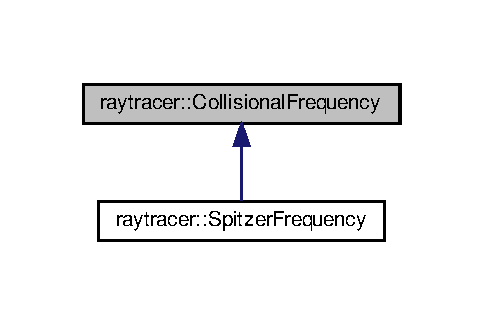
\includegraphics[width=232pt]{classraytracer_1_1CollisionalFrequency__inherit__graph}
\end{center}
\end{figure}
\subsection*{Public Member Functions}
\begin{DoxyCompactItemize}
\item 
virtual \hyperlink{structraytracer_1_1Frequency}{Frequency} \hyperlink{classraytracer_1_1CollisionalFrequency_a85c4e6175a8a692e02be34cdccbf1e16}{get} (const \hyperlink{structraytracer_1_1Density}{Density} \&density, const \hyperlink{structraytracer_1_1Temperature}{Temperature} \&temperature, const \hyperlink{structraytracer_1_1Length}{Length} \&laser\+Wavelength, double ionization) const =0
\begin{DoxyCompactList}\small\item\em Override this. \end{DoxyCompactList}\end{DoxyCompactItemize}


\subsection{Detailed Description}
Abstract interface. 

To obey this interface a method get returning the collisional frequency must be implemented. 

\subsection{Member Function Documentation}
\mbox{\Hypertarget{classraytracer_1_1CollisionalFrequency_a85c4e6175a8a692e02be34cdccbf1e16}\label{classraytracer_1_1CollisionalFrequency_a85c4e6175a8a692e02be34cdccbf1e16}} 
\index{raytracer\+::\+Collisional\+Frequency@{raytracer\+::\+Collisional\+Frequency}!get@{get}}
\index{get@{get}!raytracer\+::\+Collisional\+Frequency@{raytracer\+::\+Collisional\+Frequency}}
\subsubsection{\texorpdfstring{get()}{get()}}
{\footnotesize\ttfamily virtual \hyperlink{structraytracer_1_1Frequency}{Frequency} raytracer\+::\+Collisional\+Frequency\+::get (\begin{DoxyParamCaption}\item[{const \hyperlink{structraytracer_1_1Density}{Density} \&}]{density,  }\item[{const \hyperlink{structraytracer_1_1Temperature}{Temperature} \&}]{temperature,  }\item[{const \hyperlink{structraytracer_1_1Length}{Length} \&}]{laser\+Wavelength,  }\item[{double}]{ionization }\end{DoxyParamCaption}) const\hspace{0.3cm}{\ttfamily [pure virtual]}}



Override this. 


\begin{DoxyParams}{Parameters}
{\em density} & \\
\hline
{\em temperature} & \\
\hline
{\em laser\+Wavelength} & \\
\hline
{\em ionization} & \\
\hline
\end{DoxyParams}
\begin{DoxyReturn}{Returns}
collisional frequency given state variables 
\end{DoxyReturn}


Implemented in \hyperlink{classraytracer_1_1SpitzerFrequency_aaead0d859dd82ad4ecc0a0805af954c5}{raytracer\+::\+Spitzer\+Frequency}.



The documentation for this class was generated from the following file\+:\begin{DoxyCompactItemize}
\item 
/home/martin/\+C\+Lion\+Projects/raytracer/include/raytracer/physics/Collisional\+Frequency.\+h\end{DoxyCompactItemize}

\hypertarget{classraytracer_1_1ConstantGradient}{}\section{raytracer\+:\+:Constant\+Gradient Class Reference}
\label{classraytracer_1_1ConstantGradient}\index{raytracer\+::\+Constant\+Gradient@{raytracer\+::\+Constant\+Gradient}}


Gradient\+Calculator that returns a constant \hyperlink{classraytracer_1_1Vector}{Vector} no matter what.  




{\ttfamily \#include $<$Gradient.\+h$>$}



Inheritance diagram for raytracer\+:\+:Constant\+Gradient\+:
\nopagebreak
\begin{figure}[H]
\begin{center}
\leavevmode
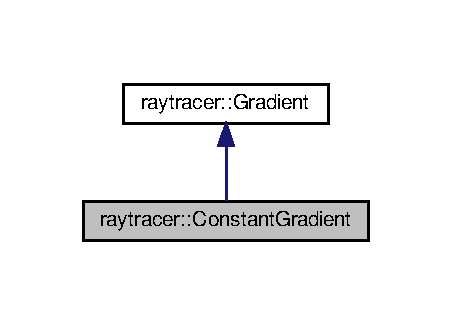
\includegraphics[width=217pt]{classraytracer_1_1ConstantGradient__inherit__graph}
\end{center}
\end{figure}


Collaboration diagram for raytracer\+:\+:Constant\+Gradient\+:
\nopagebreak
\begin{figure}[H]
\begin{center}
\leavevmode
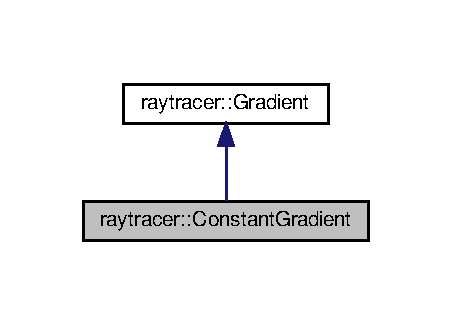
\includegraphics[width=217pt]{classraytracer_1_1ConstantGradient__coll__graph}
\end{center}
\end{figure}
\subsection*{Public Member Functions}
\begin{DoxyCompactItemize}
\item 
\hyperlink{classraytracer_1_1ConstantGradient_aa07e9f4cbdab1689e2f73d37517cd478}{Constant\+Gradient} (const \hyperlink{classraytracer_1_1Vector}{Vector} \&gradient)
\begin{DoxyCompactList}\small\item\em Constructor that takes the \hyperlink{classraytracer_1_1Vector}{Vector} that will be returned every time as parameter. \end{DoxyCompactList}\item 
\hyperlink{classraytracer_1_1Vector}{Vector} \hyperlink{classraytracer_1_1ConstantGradient_afd5e248b930551c0ad1bf84482b930b9}{get} (const \hyperlink{structraytracer_1_1PointOnFace}{Point\+On\+Face} \&point\+On\+Face, const \hyperlink{classraytracer_1_1Element}{Element} \&previous\+Element, const \hyperlink{classraytracer_1_1Element}{Element} \&next\+Element) const override
\begin{DoxyCompactList}\small\item\em Returns always the same \hyperlink{classraytracer_1_1Vector}{Vector} given at construction. \end{DoxyCompactList}\end{DoxyCompactItemize}


\subsection{Detailed Description}
Gradient\+Calculator that returns a constant \hyperlink{classraytracer_1_1Vector}{Vector} no matter what. 

\subsection{Constructor \& Destructor Documentation}
\mbox{\Hypertarget{classraytracer_1_1ConstantGradient_aa07e9f4cbdab1689e2f73d37517cd478}\label{classraytracer_1_1ConstantGradient_aa07e9f4cbdab1689e2f73d37517cd478}} 
\index{raytracer\+::\+Constant\+Gradient@{raytracer\+::\+Constant\+Gradient}!Constant\+Gradient@{Constant\+Gradient}}
\index{Constant\+Gradient@{Constant\+Gradient}!raytracer\+::\+Constant\+Gradient@{raytracer\+::\+Constant\+Gradient}}
\subsubsection{\texorpdfstring{Constant\+Gradient()}{ConstantGradient()}}
{\footnotesize\ttfamily raytracer\+::\+Constant\+Gradient\+::\+Constant\+Gradient (\begin{DoxyParamCaption}\item[{const \hyperlink{classraytracer_1_1Vector}{Vector} \&}]{gradient }\end{DoxyParamCaption})\hspace{0.3cm}{\ttfamily [explicit]}}



Constructor that takes the \hyperlink{classraytracer_1_1Vector}{Vector} that will be returned every time as parameter. 


\begin{DoxyParams}{Parameters}
{\em gradient} & -\/ the vector to be returned \\
\hline
\end{DoxyParams}


\subsection{Member Function Documentation}
\mbox{\Hypertarget{classraytracer_1_1ConstantGradient_afd5e248b930551c0ad1bf84482b930b9}\label{classraytracer_1_1ConstantGradient_afd5e248b930551c0ad1bf84482b930b9}} 
\index{raytracer\+::\+Constant\+Gradient@{raytracer\+::\+Constant\+Gradient}!get@{get}}
\index{get@{get}!raytracer\+::\+Constant\+Gradient@{raytracer\+::\+Constant\+Gradient}}
\subsubsection{\texorpdfstring{get()}{get()}}
{\footnotesize\ttfamily \hyperlink{classraytracer_1_1Vector}{Vector} raytracer\+::\+Constant\+Gradient\+::get (\begin{DoxyParamCaption}\item[{const \hyperlink{structraytracer_1_1PointOnFace}{Point\+On\+Face} \&}]{point\+On\+Face,  }\item[{const \hyperlink{classraytracer_1_1Element}{Element} \&}]{previous\+Element,  }\item[{const \hyperlink{classraytracer_1_1Element}{Element} \&}]{next\+Element }\end{DoxyParamCaption}) const\hspace{0.3cm}{\ttfamily [override]}, {\ttfamily [virtual]}}



Returns always the same \hyperlink{classraytracer_1_1Vector}{Vector} given at construction. 

\begin{DoxyReturn}{Returns}
vector gradient. 
\end{DoxyReturn}


Implements \hyperlink{classraytracer_1_1Gradient_a93ccfef0662634c5f9a3c8dd04e73496}{raytracer\+::\+Gradient}.



The documentation for this class was generated from the following file\+:\begin{DoxyCompactItemize}
\item 
/home/martin/\+C\+Lion\+Projects/raytracer/include/raytracer/physics/Gradient.\+h\end{DoxyCompactItemize}

\hypertarget{structraytracer_1_1ContinueStraight}{}\section{raytracer\+:\+:Continue\+Straight Struct Reference}
\label{structraytracer_1_1ContinueStraight}\index{raytracer\+::\+Continue\+Straight@{raytracer\+::\+Continue\+Straight}}


Functor that returns always the previous\+Direction.  




{\ttfamily \#include $<$Refraction.\+h$>$}

\subsection*{Public Member Functions}
\begin{DoxyCompactItemize}
\item 
\hyperlink{classraytracer_1_1Vector}{Vector} \hyperlink{structraytracer_1_1ContinueStraight_ad985691646c9dea102f182862750b071}{operator()} (const \hyperlink{structraytracer_1_1PointOnFace}{Point\+On\+Face} \&, const \hyperlink{classraytracer_1_1Vector}{Vector} \&previous\+Direction, const \hyperlink{classraytracer_1_1Element}{Element} \&, const \hyperlink{classraytracer_1_1Element}{Element} \&, const \hyperlink{classraytracer_1_1LaserRay}{Laser\+Ray} \&)
\begin{DoxyCompactList}\small\item\em Function to be used in \hyperlink{classraytracer_1_1Laser_a40fd2b112fb1de646861d7e93ac303e3}{Laser\+::generate\+Intersections()} as find\+Direction. \end{DoxyCompactList}\end{DoxyCompactItemize}


\subsection{Detailed Description}
Functor that returns always the previous\+Direction. 

\subsection{Member Function Documentation}
\mbox{\Hypertarget{structraytracer_1_1ContinueStraight_ad985691646c9dea102f182862750b071}\label{structraytracer_1_1ContinueStraight_ad985691646c9dea102f182862750b071}} 
\index{raytracer\+::\+Continue\+Straight@{raytracer\+::\+Continue\+Straight}!operator()@{operator()}}
\index{operator()@{operator()}!raytracer\+::\+Continue\+Straight@{raytracer\+::\+Continue\+Straight}}
\subsubsection{\texorpdfstring{operator()()}{operator()()}}
{\footnotesize\ttfamily \hyperlink{classraytracer_1_1Vector}{Vector} raytracer\+::\+Continue\+Straight\+::operator() (\begin{DoxyParamCaption}\item[{const \hyperlink{structraytracer_1_1PointOnFace}{Point\+On\+Face} \&}]{,  }\item[{const \hyperlink{classraytracer_1_1Vector}{Vector} \&}]{previous\+Direction,  }\item[{const \hyperlink{classraytracer_1_1Element}{Element} \&}]{,  }\item[{const \hyperlink{classraytracer_1_1Element}{Element} \&}]{,  }\item[{const \hyperlink{classraytracer_1_1LaserRay}{Laser\+Ray} \&}]{ }\end{DoxyParamCaption})\hspace{0.3cm}{\ttfamily [inline]}}



Function to be used in \hyperlink{classraytracer_1_1Laser_a40fd2b112fb1de646861d7e93ac303e3}{Laser\+::generate\+Intersections()} as find\+Direction. 

It returns the previous\+Direction given, effectively continuing in a straight line. 
\begin{DoxyParams}{Parameters}
{\em previous\+Direction} & \\
\hline
\end{DoxyParams}
\begin{DoxyReturn}{Returns}
previous\+Direction 
\end{DoxyReturn}


The documentation for this struct was generated from the following file\+:\begin{DoxyCompactItemize}
\item 
/home/martin/\+C\+Lion\+Projects/raytracer/include/raytracer/physics/Refraction.\+h\end{DoxyCompactItemize}

\hypertarget{structraytracer_1_1Density}{}\section{raytracer\+:\+:Density Struct Reference}
\label{structraytracer_1_1Density}\index{raytracer\+::\+Density@{raytracer\+::\+Density}}


Strong type representing length in cm$^\wedge$-\/3.  




{\ttfamily \#include $<$Magnitudes.\+h$>$}



\subsection{Detailed Description}
Strong type representing length in cm$^\wedge$-\/3. 



The documentation for this struct was generated from the following file\+:\begin{DoxyCompactItemize}
\item 
/home/martin/\+C\+Lion\+Projects/raytracer/include/raytracer/physics/Magnitudes.\+h\end{DoxyCompactItemize}

\hypertarget{structraytracer_1_1DiscreteLine}{}\section{raytracer\+:\+:Discrete\+Line Struct Reference}
\label{structraytracer_1_1DiscreteLine}\index{raytracer\+::\+Discrete\+Line@{raytracer\+::\+Discrete\+Line}}


Structure representing a discretization of a distance.  




{\ttfamily \#include $<$Mesh.\+h$>$}

\subsection*{Public Attributes}
\begin{DoxyCompactItemize}
\item 
double \hyperlink{structraytracer_1_1DiscreteLine_a9a6dc228b1d824f485f2e94965e7fe9a}{length}
\begin{DoxyCompactList}\small\item\em How long is the line. \end{DoxyCompactList}\item 
size\+\_\+t \hyperlink{structraytracer_1_1DiscreteLine_a80395f9fb7bed884f348199fca0f1ccf}{segment\+Count}
\begin{DoxyCompactList}\small\item\em Number of segments on the line. \end{DoxyCompactList}\end{DoxyCompactItemize}


\subsection{Detailed Description}
Structure representing a discretization of a distance. 

That is how many same size segments are on the line with given width. 

\subsection{Member Data Documentation}
\mbox{\Hypertarget{structraytracer_1_1DiscreteLine_a9a6dc228b1d824f485f2e94965e7fe9a}\label{structraytracer_1_1DiscreteLine_a9a6dc228b1d824f485f2e94965e7fe9a}} 
\index{raytracer\+::\+Discrete\+Line@{raytracer\+::\+Discrete\+Line}!length@{length}}
\index{length@{length}!raytracer\+::\+Discrete\+Line@{raytracer\+::\+Discrete\+Line}}
\subsubsection{\texorpdfstring{length}{length}}
{\footnotesize\ttfamily double raytracer\+::\+Discrete\+Line\+::length}



How long is the line. 

\mbox{\Hypertarget{structraytracer_1_1DiscreteLine_a80395f9fb7bed884f348199fca0f1ccf}\label{structraytracer_1_1DiscreteLine_a80395f9fb7bed884f348199fca0f1ccf}} 
\index{raytracer\+::\+Discrete\+Line@{raytracer\+::\+Discrete\+Line}!segment\+Count@{segment\+Count}}
\index{segment\+Count@{segment\+Count}!raytracer\+::\+Discrete\+Line@{raytracer\+::\+Discrete\+Line}}
\subsubsection{\texorpdfstring{segment\+Count}{segmentCount}}
{\footnotesize\ttfamily size\+\_\+t raytracer\+::\+Discrete\+Line\+::segment\+Count}



Number of segments on the line. 

Eg. \hyperlink{structraytracer_1_1DiscreteLine}{Discrete\+Line} split by two points has three segments. 

The documentation for this struct was generated from the following file\+:\begin{DoxyCompactItemize}
\item 
/home/martin/\+C\+Lion\+Projects/raytracer/include/raytracer/geometry/Mesh.\+h\end{DoxyCompactItemize}

\hypertarget{structraytracer_1_1DontStop}{}\section{raytracer\+:\+:Dont\+Stop Struct Reference}
\label{structraytracer_1_1DontStop}\index{raytracer\+::\+Dont\+Stop@{raytracer\+::\+Dont\+Stop}}


Functor for ray propagation that returns false in any case.  




{\ttfamily \#include $<$Termination.\+h$>$}

\subsection*{Public Member Functions}
\begin{DoxyCompactItemize}
\item 
bool \hyperlink{structraytracer_1_1DontStop_a1b7c7429e15c8aced0dd2a0d296c2e17}{operator()} (const \hyperlink{classraytracer_1_1Element}{Element} \&, const \hyperlink{classraytracer_1_1LaserRay}{Laser\+Ray} \&)
\begin{DoxyCompactList}\small\item\em Just returns false. \end{DoxyCompactList}\end{DoxyCompactItemize}


\subsection{Detailed Description}
Functor for ray propagation that returns false in any case. 

Convenience struct to keep the call similar to eg. \hyperlink{structraytracer_1_1StopAtCritical}{Stop\+At\+Critical}. 

\subsection{Member Function Documentation}
\mbox{\Hypertarget{structraytracer_1_1DontStop_a1b7c7429e15c8aced0dd2a0d296c2e17}\label{structraytracer_1_1DontStop_a1b7c7429e15c8aced0dd2a0d296c2e17}} 
\index{raytracer\+::\+Dont\+Stop@{raytracer\+::\+Dont\+Stop}!operator()@{operator()}}
\index{operator()@{operator()}!raytracer\+::\+Dont\+Stop@{raytracer\+::\+Dont\+Stop}}
\subsubsection{\texorpdfstring{operator()()}{operator()()}}
{\footnotesize\ttfamily bool raytracer\+::\+Dont\+Stop\+::operator() (\begin{DoxyParamCaption}\item[{const \hyperlink{classraytracer_1_1Element}{Element} \&}]{,  }\item[{const \hyperlink{classraytracer_1_1LaserRay}{Laser\+Ray} \&}]{ }\end{DoxyParamCaption})}



Just returns false. 

\begin{DoxyReturn}{Returns}
false. 
\end{DoxyReturn}


The documentation for this struct was generated from the following file\+:\begin{DoxyCompactItemize}
\item 
/home/martin/\+C\+Lion\+Projects/raytracer/include/raytracer/physics/Termination.\+h\end{DoxyCompactItemize}

\hypertarget{classraytracer_1_1Element}{}\section{raytracer\+:\+:Element Class Reference}
\label{classraytracer_1_1Element}\index{raytracer\+::\+Element@{raytracer\+::\+Element}}


Class representing a single polygonal element in mesh.  




{\ttfamily \#include $<$Element.\+h$>$}

\subsection*{Public Member Functions}
\begin{DoxyCompactItemize}
\item 
const std\+::vector$<$ \hyperlink{classraytracer_1_1Face}{Face} $\ast$ $>$ \& \hyperlink{classraytracer_1_1Element_a46d4135d6ef7fd7c34656aa90f35b2ed}{get\+Faces} () const
\begin{DoxyCompactList}\small\item\em Get the faces of the \hyperlink{classraytracer_1_1Element}{Element}. \end{DoxyCompactList}\item 
\hyperlink{classraytracer_1_1Element_a70169ab8330ac32971e0925ae4ad2fd9}{Element} (int id, std\+::vector$<$ \hyperlink{classraytracer_1_1Face}{Face} $\ast$$>$ faces)
\begin{DoxyCompactList}\small\item\em Constructor taking an id and std\+::vector of faces of the element. \end{DoxyCompactList}\item 
int \hyperlink{classraytracer_1_1Element_ab56fe71038371416a91db232b27c006a}{get\+Id} () const
\begin{DoxyCompactList}\small\item\em Retrieve the id of element. \end{DoxyCompactList}\end{DoxyCompactItemize}


\subsection{Detailed Description}
Class representing a single polygonal element in mesh. 

Could be 2\+D/3D given by set of faces (edges, surfaces). \begin{DoxyWarning}{Warning}
Do not construct this manually unless you know what you are doing. 
\end{DoxyWarning}


\subsection{Constructor \& Destructor Documentation}
\mbox{\Hypertarget{classraytracer_1_1Element_a70169ab8330ac32971e0925ae4ad2fd9}\label{classraytracer_1_1Element_a70169ab8330ac32971e0925ae4ad2fd9}} 
\index{raytracer\+::\+Element@{raytracer\+::\+Element}!Element@{Element}}
\index{Element@{Element}!raytracer\+::\+Element@{raytracer\+::\+Element}}
\subsubsection{\texorpdfstring{Element()}{Element()}}
{\footnotesize\ttfamily raytracer\+::\+Element\+::\+Element (\begin{DoxyParamCaption}\item[{int}]{id,  }\item[{std\+::vector$<$ \hyperlink{classraytracer_1_1Face}{Face} $\ast$$>$}]{faces }\end{DoxyParamCaption})\hspace{0.3cm}{\ttfamily [explicit]}}



Constructor taking an id and std\+::vector of faces of the element. 

\begin{DoxyWarning}{Warning}
It is users responsibility for the id to be unique. It is thus advised to not construct instance of \hyperlink{classraytracer_1_1Element}{Element} manually.
\end{DoxyWarning}
Clockwise order of faces is preferred in 2D. 
\begin{DoxyParams}{Parameters}
{\em id} & unique identification \\
\hline
{\em faces} & of the element \\
\hline
\end{DoxyParams}


\subsection{Member Function Documentation}
\mbox{\Hypertarget{classraytracer_1_1Element_a46d4135d6ef7fd7c34656aa90f35b2ed}\label{classraytracer_1_1Element_a46d4135d6ef7fd7c34656aa90f35b2ed}} 
\index{raytracer\+::\+Element@{raytracer\+::\+Element}!get\+Faces@{get\+Faces}}
\index{get\+Faces@{get\+Faces}!raytracer\+::\+Element@{raytracer\+::\+Element}}
\subsubsection{\texorpdfstring{get\+Faces()}{getFaces()}}
{\footnotesize\ttfamily const std\+::vector$<$\hyperlink{classraytracer_1_1Face}{Face} $\ast$$>$\& raytracer\+::\+Element\+::get\+Faces (\begin{DoxyParamCaption}{ }\end{DoxyParamCaption}) const}



Get the faces of the \hyperlink{classraytracer_1_1Element}{Element}. 

Edges in 2D, surfaces in 3D. \begin{DoxyReturn}{Returns}
the faces 
\end{DoxyReturn}
\mbox{\Hypertarget{classraytracer_1_1Element_ab56fe71038371416a91db232b27c006a}\label{classraytracer_1_1Element_ab56fe71038371416a91db232b27c006a}} 
\index{raytracer\+::\+Element@{raytracer\+::\+Element}!get\+Id@{get\+Id}}
\index{get\+Id@{get\+Id}!raytracer\+::\+Element@{raytracer\+::\+Element}}
\subsubsection{\texorpdfstring{get\+Id()}{getId()}}
{\footnotesize\ttfamily int raytracer\+::\+Element\+::get\+Id (\begin{DoxyParamCaption}{ }\end{DoxyParamCaption}) const}



Retrieve the id of element. 

\begin{DoxyReturn}{Returns}
id 
\end{DoxyReturn}


The documentation for this class was generated from the following file\+:\begin{DoxyCompactItemize}
\item 
/home/martin/\+C\+Lion\+Projects/raytracer/include/raytracer/geometry/Element.\+h\end{DoxyCompactItemize}

\hypertarget{structraytracer_1_1Energy}{}\section{raytracer\+:\+:Energy Struct Reference}
\label{structraytracer_1_1Energy}\index{raytracer\+::\+Energy@{raytracer\+::\+Energy}}


Strong type representing energy in joules.  




{\ttfamily \#include $<$Magnitudes.\+h$>$}



\subsection{Detailed Description}
Strong type representing energy in joules. 



The documentation for this struct was generated from the following file\+:\begin{DoxyCompactItemize}
\item 
/home/martin/\+C\+Lion\+Projects/raytracer/include/raytracer/physics/Magnitudes.\+h\end{DoxyCompactItemize}

\hypertarget{classraytracer_1_1Face}{}\section{raytracer\+:\+:Face Class Reference}
\label{classraytracer_1_1Face}\index{raytracer\+::\+Face@{raytracer\+::\+Face}}


Class representing a polygonal face in mesh (edge in 2D, surface polygon face in 3D).  




{\ttfamily \#include $<$Face.\+h$>$}

\subsection*{Public Member Functions}
\begin{DoxyCompactItemize}
\item 
\hyperlink{classraytracer_1_1Vector}{Vector} \hyperlink{classraytracer_1_1Face_a4b7079a236be6c724a160250eccf3bac}{get\+Normal} () const
\begin{DoxyCompactList}\small\item\em Calculate a normal to the face (edge in 2D). \end{DoxyCompactList}\item 
const std\+::vector$<$ \hyperlink{classraytracer_1_1Point}{Point} $\ast$ $>$ \& \hyperlink{classraytracer_1_1Face_a54b2f1c95ee3d187ca286e7519450af0}{get\+Points} () const
\begin{DoxyCompactList}\small\item\em Get the points forming the face. \end{DoxyCompactList}\item 
\hyperlink{classraytracer_1_1Face_ad1d772053e4782fe0291df924d3beffe}{Face} (int id, std\+::vector$<$ \hyperlink{classraytracer_1_1Point}{Point} $\ast$$>$ points)
\begin{DoxyCompactList}\small\item\em Construct the face using an id and std\+::vector of points that the face consist of. \end{DoxyCompactList}\item 
int \hyperlink{classraytracer_1_1Face_a1693a7b1269bea1cb1e9ce72f1d10c04}{get\+Id} () const
\begin{DoxyCompactList}\small\item\em Get the id of the face. \end{DoxyCompactList}\end{DoxyCompactItemize}


\subsection{Detailed Description}
Class representing a polygonal face in mesh (edge in 2D, surface polygon face in 3D). 

\begin{DoxyWarning}{Warning}
Do not construct this manually unless you know what you are doing. 
\end{DoxyWarning}


\subsection{Constructor \& Destructor Documentation}
\mbox{\Hypertarget{classraytracer_1_1Face_ad1d772053e4782fe0291df924d3beffe}\label{classraytracer_1_1Face_ad1d772053e4782fe0291df924d3beffe}} 
\index{raytracer\+::\+Face@{raytracer\+::\+Face}!Face@{Face}}
\index{Face@{Face}!raytracer\+::\+Face@{raytracer\+::\+Face}}
\subsubsection{\texorpdfstring{Face()}{Face()}}
{\footnotesize\ttfamily raytracer\+::\+Face\+::\+Face (\begin{DoxyParamCaption}\item[{int}]{id,  }\item[{std\+::vector$<$ \hyperlink{classraytracer_1_1Point}{Point} $\ast$$>$}]{points }\end{DoxyParamCaption})\hspace{0.3cm}{\ttfamily [explicit]}}



Construct the face using an id and std\+::vector of points that the face consist of. 

\begin{DoxyWarning}{Warning}
It is users responsibility for the id to be unique. It is thus advised to not construct instance of \hyperlink{classraytracer_1_1Face}{Face} manually.
\end{DoxyWarning}

\begin{DoxyParams}{Parameters}
{\em id} & unique identification \\
\hline
{\em points} & the face consists of \\
\hline
\end{DoxyParams}


\subsection{Member Function Documentation}
\mbox{\Hypertarget{classraytracer_1_1Face_a1693a7b1269bea1cb1e9ce72f1d10c04}\label{classraytracer_1_1Face_a1693a7b1269bea1cb1e9ce72f1d10c04}} 
\index{raytracer\+::\+Face@{raytracer\+::\+Face}!get\+Id@{get\+Id}}
\index{get\+Id@{get\+Id}!raytracer\+::\+Face@{raytracer\+::\+Face}}
\subsubsection{\texorpdfstring{get\+Id()}{getId()}}
{\footnotesize\ttfamily int raytracer\+::\+Face\+::get\+Id (\begin{DoxyParamCaption}{ }\end{DoxyParamCaption}) const}



Get the id of the face. 

\begin{DoxyReturn}{Returns}
id 
\end{DoxyReturn}
\mbox{\Hypertarget{classraytracer_1_1Face_a4b7079a236be6c724a160250eccf3bac}\label{classraytracer_1_1Face_a4b7079a236be6c724a160250eccf3bac}} 
\index{raytracer\+::\+Face@{raytracer\+::\+Face}!get\+Normal@{get\+Normal}}
\index{get\+Normal@{get\+Normal}!raytracer\+::\+Face@{raytracer\+::\+Face}}
\subsubsection{\texorpdfstring{get\+Normal()}{getNormal()}}
{\footnotesize\ttfamily \hyperlink{classraytracer_1_1Vector}{Vector} raytracer\+::\+Face\+::get\+Normal (\begin{DoxyParamCaption}{ }\end{DoxyParamCaption}) const}



Calculate a normal to the face (edge in 2D). 

By convention in 2D, the normal is outward for points in clockwise order forming a polygon. \begin{DoxyReturn}{Returns}
the normal vector. 
\end{DoxyReturn}
\mbox{\Hypertarget{classraytracer_1_1Face_a54b2f1c95ee3d187ca286e7519450af0}\label{classraytracer_1_1Face_a54b2f1c95ee3d187ca286e7519450af0}} 
\index{raytracer\+::\+Face@{raytracer\+::\+Face}!get\+Points@{get\+Points}}
\index{get\+Points@{get\+Points}!raytracer\+::\+Face@{raytracer\+::\+Face}}
\subsubsection{\texorpdfstring{get\+Points()}{getPoints()}}
{\footnotesize\ttfamily const std\+::vector$<$\hyperlink{classraytracer_1_1Point}{Point} $\ast$$>$\& raytracer\+::\+Face\+::get\+Points (\begin{DoxyParamCaption}{ }\end{DoxyParamCaption}) const}



Get the points forming the face. 

\begin{DoxyReturn}{Returns}
the points. 
\end{DoxyReturn}


The documentation for this class was generated from the following file\+:\begin{DoxyCompactItemize}
\item 
/home/martin/\+C\+Lion\+Projects/raytracer/include/raytracer/geometry/Face.\+h\end{DoxyCompactItemize}

\hypertarget{structraytracer_1_1Frequency}{}\section{raytracer\+:\+:Frequency Struct Reference}
\label{structraytracer_1_1Frequency}\index{raytracer\+::\+Frequency@{raytracer\+::\+Frequency}}


Strong type representing frequency in s$^\wedge$-\/1.  




{\ttfamily \#include $<$Magnitudes.\+h$>$}



\subsection{Detailed Description}
Strong type representing frequency in s$^\wedge$-\/1. 



The documentation for this struct was generated from the following file\+:\begin{DoxyCompactItemize}
\item 
/home/martin/\+C\+Lion\+Projects/raytracer/include/raytracer/physics/Magnitudes.\+h\end{DoxyCompactItemize}

\hypertarget{classraytracer_1_1Gaussian}{}\section{raytracer\+:\+:Gaussian Class Reference}
\label{classraytracer_1_1Gaussian}\index{raytracer\+::\+Gaussian@{raytracer\+::\+Gaussian}}


Class representing a 1D gaussian with given parametrs.  




{\ttfamily \#include $<$Free\+Functions.\+h$>$}

\subsection*{Public Member Functions}
\begin{DoxyCompactItemize}
\item 
\hyperlink{classraytracer_1_1Gaussian_ac8b11a424ae009492e40351452a77949}{Gaussian} (double F\+W\+HM, double maximum=1, double center=0)
\begin{DoxyCompactList}\small\item\em Construct the gaussian using F\+W\+HM, value at maxim (also the value of the integral) and the center point. \end{DoxyCompactList}\item 
double \hyperlink{classraytracer_1_1Gaussian_ac4bbe17132daa8b89dc431c353efc205}{operator()} (double x)
\begin{DoxyCompactList}\small\item\em Value of the gaussian at given point x. \end{DoxyCompactList}\end{DoxyCompactItemize}


\subsection{Detailed Description}
Class representing a 1D gaussian with given parametrs. 

\subsection{Constructor \& Destructor Documentation}
\mbox{\Hypertarget{classraytracer_1_1Gaussian_ac8b11a424ae009492e40351452a77949}\label{classraytracer_1_1Gaussian_ac8b11a424ae009492e40351452a77949}} 
\index{raytracer\+::\+Gaussian@{raytracer\+::\+Gaussian}!Gaussian@{Gaussian}}
\index{Gaussian@{Gaussian}!raytracer\+::\+Gaussian@{raytracer\+::\+Gaussian}}
\subsubsection{\texorpdfstring{Gaussian()}{Gaussian()}}
{\footnotesize\ttfamily raytracer\+::\+Gaussian\+::\+Gaussian (\begin{DoxyParamCaption}\item[{double}]{F\+W\+HM,  }\item[{double}]{maximum = {\ttfamily 1},  }\item[{double}]{center = {\ttfamily 0} }\end{DoxyParamCaption})\hspace{0.3cm}{\ttfamily [explicit]}}



Construct the gaussian using F\+W\+HM, value at maxim (also the value of the integral) and the center point. 


\begin{DoxyParams}{Parameters}
{\em F\+W\+HM} & \\
\hline
{\em maximum} & or also the intgral value \\
\hline
{\em center} & point \\
\hline
\end{DoxyParams}


\subsection{Member Function Documentation}
\mbox{\Hypertarget{classraytracer_1_1Gaussian_ac4bbe17132daa8b89dc431c353efc205}\label{classraytracer_1_1Gaussian_ac4bbe17132daa8b89dc431c353efc205}} 
\index{raytracer\+::\+Gaussian@{raytracer\+::\+Gaussian}!operator()@{operator()}}
\index{operator()@{operator()}!raytracer\+::\+Gaussian@{raytracer\+::\+Gaussian}}
\subsubsection{\texorpdfstring{operator()()}{operator()()}}
{\footnotesize\ttfamily double raytracer\+::\+Gaussian\+::operator() (\begin{DoxyParamCaption}\item[{double}]{x }\end{DoxyParamCaption})}



Value of the gaussian at given point x. 


\begin{DoxyParams}{Parameters}
{\em x} & \\
\hline
\end{DoxyParams}
\begin{DoxyReturn}{Returns}
the value 
\end{DoxyReturn}


The documentation for this class was generated from the following file\+:\begin{DoxyCompactItemize}
\item 
/home/martin/\+C\+Lion\+Projects/raytracer/include/raytracer/utility/Free\+Functions.\+h\end{DoxyCompactItemize}

\hypertarget{classraytracer_1_1Gradient}{}\section{raytracer\+:\+:Gradient Class Reference}
\label{classraytracer_1_1Gradient}\index{raytracer\+::\+Gradient@{raytracer\+::\+Gradient}}


Abstract interface to provide a Gradient\+Calculator.  




{\ttfamily \#include $<$Gradient.\+h$>$}



Inheritance diagram for raytracer\+:\+:Gradient\+:
\nopagebreak
\begin{figure}[H]
\begin{center}
\leavevmode
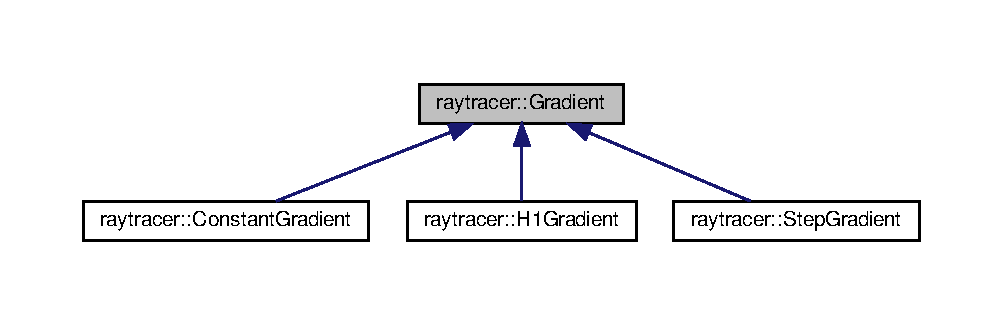
\includegraphics[width=350pt]{classraytracer_1_1Gradient__inherit__graph}
\end{center}
\end{figure}
\subsection*{Public Member Functions}
\begin{DoxyCompactItemize}
\item 
virtual \hyperlink{classraytracer_1_1Vector}{Vector} \hyperlink{classraytracer_1_1Gradient_a93ccfef0662634c5f9a3c8dd04e73496}{get} (const \hyperlink{structraytracer_1_1PointOnFace}{Point\+On\+Face} \&point\+On\+Face, const \hyperlink{classraytracer_1_1Element}{Element} \&previous\+Element, const \hyperlink{classraytracer_1_1Element}{Element} \&next\+Element) const =0
\begin{DoxyCompactList}\small\item\em Override this. \end{DoxyCompactList}\end{DoxyCompactItemize}


\subsection{Detailed Description}
Abstract interface to provide a Gradient\+Calculator. 

To obey this interface implement the get method. 

\subsection{Member Function Documentation}
\mbox{\Hypertarget{classraytracer_1_1Gradient_a93ccfef0662634c5f9a3c8dd04e73496}\label{classraytracer_1_1Gradient_a93ccfef0662634c5f9a3c8dd04e73496}} 
\index{raytracer\+::\+Gradient@{raytracer\+::\+Gradient}!get@{get}}
\index{get@{get}!raytracer\+::\+Gradient@{raytracer\+::\+Gradient}}
\subsubsection{\texorpdfstring{get()}{get()}}
{\footnotesize\ttfamily virtual \hyperlink{classraytracer_1_1Vector}{Vector} raytracer\+::\+Gradient\+::get (\begin{DoxyParamCaption}\item[{const \hyperlink{structraytracer_1_1PointOnFace}{Point\+On\+Face} \&}]{point\+On\+Face,  }\item[{const \hyperlink{classraytracer_1_1Element}{Element} \&}]{previous\+Element,  }\item[{const \hyperlink{classraytracer_1_1Element}{Element} \&}]{next\+Element }\end{DoxyParamCaption}) const\hspace{0.3cm}{\ttfamily [pure virtual]}}



Override this. 

\begin{DoxyReturn}{Returns}
the gradient at given intersection \hyperlink{structraytracer_1_1PointOnFace}{Point\+On\+Face}. 
\end{DoxyReturn}


Implemented in \hyperlink{classraytracer_1_1StepGradient_a0c18f1abff911e8ebd91184b55c8c0ef}{raytracer\+::\+Step\+Gradient}, \hyperlink{classraytracer_1_1H1Gradient_a7c847fef0d9cb6fbd143552acace82a5}{raytracer\+::\+H1\+Gradient}, and \hyperlink{classraytracer_1_1ConstantGradient_afd5e248b930551c0ad1bf84482b930b9}{raytracer\+::\+Constant\+Gradient}.



The documentation for this class was generated from the following file\+:\begin{DoxyCompactItemize}
\item 
/home/martin/\+C\+Lion\+Projects/raytracer/include/raytracer/physics/Gradient.\+h\end{DoxyCompactItemize}

\hypertarget{classraytracer_1_1H1Gradient}{}\section{raytracer\+:\+:H1\+Gradient Class Reference}
\label{classraytracer_1_1H1Gradient}\index{raytracer\+::\+H1\+Gradient@{raytracer\+::\+H1\+Gradient}}


Gradient\+Calculator that stores a density grid function defined in H1 space obtained from function given if L2.  




{\ttfamily \#include $<$Gradient.\+h$>$}



Inheritance diagram for raytracer\+:\+:H1\+Gradient\+:
\nopagebreak
\begin{figure}[H]
\begin{center}
\leavevmode
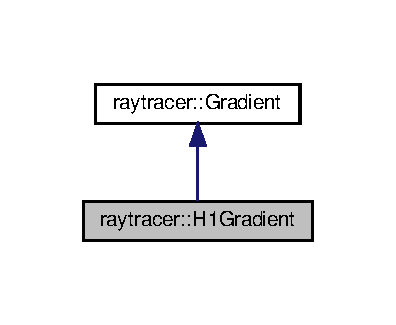
\includegraphics[width=190pt]{classraytracer_1_1H1Gradient__inherit__graph}
\end{center}
\end{figure}


Collaboration diagram for raytracer\+:\+:H1\+Gradient\+:
\nopagebreak
\begin{figure}[H]
\begin{center}
\leavevmode
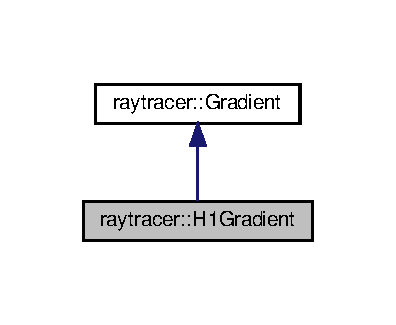
\includegraphics[width=190pt]{classraytracer_1_1H1Gradient__coll__graph}
\end{center}
\end{figure}
\subsection*{Public Member Functions}
\begin{DoxyCompactItemize}
\item 
\hyperlink{classraytracer_1_1H1Gradient_a7499a9dcb45b6c813b09fe14d08d98e4}{H1\+Gradient} (mfem\+::\+Finite\+Element\+Space \&l2\+Space, mfem\+::\+Finite\+Element\+Space \&h1\+Space)
\begin{DoxyCompactList}\small\item\em Constructor that expects the l2 and h1 spaces. \end{DoxyCompactList}\item 
\hyperlink{classraytracer_1_1Vector}{Vector} \hyperlink{classraytracer_1_1H1Gradient_a7c847fef0d9cb6fbd143552acace82a5}{get} (const \hyperlink{structraytracer_1_1PointOnFace}{Point\+On\+Face} \&point\+On\+Face, const \hyperlink{classraytracer_1_1Element}{Element} \&previous\+Element, const \hyperlink{classraytracer_1_1Element}{Element} \&next\+Element) const override
\begin{DoxyCompactList}\small\item\em Return the value of gradient at the intersection point. \end{DoxyCompactList}\item 
void \hyperlink{classraytracer_1_1H1Gradient_a3a6918392cf6b2113061626400ef883a}{update\+Density} (mfem\+::\+Grid\+Function \&density)
\begin{DoxyCompactList}\small\item\em Update the density from which the gradient is calculated. \end{DoxyCompactList}\end{DoxyCompactItemize}


\subsection{Detailed Description}
Gradient\+Calculator that stores a density grid function defined in H1 space obtained from function given if L2. 

When get is called the gradient of this function is calculated at given point.

\begin{DoxyWarning}{Warning}
Please note that \hyperlink{classraytracer_1_1H1Gradient_a3a6918392cf6b2113061626400ef883a}{update\+Density()} must be called before calling \hyperlink{classraytracer_1_1H1Gradient_a7c847fef0d9cb6fbd143552acace82a5}{get()}. 
\end{DoxyWarning}


\subsection{Constructor \& Destructor Documentation}
\mbox{\Hypertarget{classraytracer_1_1H1Gradient_a7499a9dcb45b6c813b09fe14d08d98e4}\label{classraytracer_1_1H1Gradient_a7499a9dcb45b6c813b09fe14d08d98e4}} 
\index{raytracer\+::\+H1\+Gradient@{raytracer\+::\+H1\+Gradient}!H1\+Gradient@{H1\+Gradient}}
\index{H1\+Gradient@{H1\+Gradient}!raytracer\+::\+H1\+Gradient@{raytracer\+::\+H1\+Gradient}}
\subsubsection{\texorpdfstring{H1\+Gradient()}{H1Gradient()}}
{\footnotesize\ttfamily raytracer\+::\+H1\+Gradient\+::\+H1\+Gradient (\begin{DoxyParamCaption}\item[{mfem\+::\+Finite\+Element\+Space \&}]{l2\+Space,  }\item[{mfem\+::\+Finite\+Element\+Space \&}]{h1\+Space }\end{DoxyParamCaption})}



Constructor that expects the l2 and h1 spaces. 

L2 is the space in which density is usually defined and H1 is the space into which the density is transformed to be able to evaluate gradient. 
\begin{DoxyParams}{Parameters}
{\em l2\+Space} & \\
\hline
{\em h1\+Space} & \\
\hline
\end{DoxyParams}


\subsection{Member Function Documentation}
\mbox{\Hypertarget{classraytracer_1_1H1Gradient_a7c847fef0d9cb6fbd143552acace82a5}\label{classraytracer_1_1H1Gradient_a7c847fef0d9cb6fbd143552acace82a5}} 
\index{raytracer\+::\+H1\+Gradient@{raytracer\+::\+H1\+Gradient}!get@{get}}
\index{get@{get}!raytracer\+::\+H1\+Gradient@{raytracer\+::\+H1\+Gradient}}
\subsubsection{\texorpdfstring{get()}{get()}}
{\footnotesize\ttfamily \hyperlink{classraytracer_1_1Vector}{Vector} raytracer\+::\+H1\+Gradient\+::get (\begin{DoxyParamCaption}\item[{const \hyperlink{structraytracer_1_1PointOnFace}{Point\+On\+Face} \&}]{point\+On\+Face,  }\item[{const \hyperlink{classraytracer_1_1Element}{Element} \&}]{previous\+Element,  }\item[{const \hyperlink{classraytracer_1_1Element}{Element} \&}]{next\+Element }\end{DoxyParamCaption}) const\hspace{0.3cm}{\ttfamily [override]}, {\ttfamily [virtual]}}



Return the value of gradient at the intersection point. 


\begin{DoxyParams}{Parameters}
{\em point\+On\+Face} & \\
\hline
{\em previous\+Element} & \\
\hline
{\em next\+Element} & \\
\hline
\end{DoxyParams}
\begin{DoxyReturn}{Returns}
gradient at given point 
\end{DoxyReturn}


Implements \hyperlink{classraytracer_1_1Gradient_a93ccfef0662634c5f9a3c8dd04e73496}{raytracer\+::\+Gradient}.

\mbox{\Hypertarget{classraytracer_1_1H1Gradient_a3a6918392cf6b2113061626400ef883a}\label{classraytracer_1_1H1Gradient_a3a6918392cf6b2113061626400ef883a}} 
\index{raytracer\+::\+H1\+Gradient@{raytracer\+::\+H1\+Gradient}!update\+Density@{update\+Density}}
\index{update\+Density@{update\+Density}!raytracer\+::\+H1\+Gradient@{raytracer\+::\+H1\+Gradient}}
\subsubsection{\texorpdfstring{update\+Density()}{updateDensity()}}
{\footnotesize\ttfamily void raytracer\+::\+H1\+Gradient\+::update\+Density (\begin{DoxyParamCaption}\item[{mfem\+::\+Grid\+Function \&}]{density }\end{DoxyParamCaption})}



Update the density from which the gradient is calculated. 

The density should be a function in L2 space. 
\begin{DoxyParams}{Parameters}
{\em density} & defined over L2 \\
\hline
\end{DoxyParams}


The documentation for this class was generated from the following file\+:\begin{DoxyCompactItemize}
\item 
/home/martin/\+C\+Lion\+Projects/raytracer/include/raytracer/physics/Gradient.\+h\end{DoxyCompactItemize}

\hypertarget{structraytracer_1_1HalfLine}{}\section{raytracer\+:\+:Half\+Line Struct Reference}
\label{structraytracer_1_1HalfLine}\index{raytracer\+::\+Half\+Line@{raytracer\+::\+Half\+Line}}


Structure representing a half line.  




{\ttfamily \#include $<$Intersection.\+h$>$}



Collaboration diagram for raytracer\+:\+:Half\+Line\+:
\nopagebreak
\begin{figure}[H]
\begin{center}
\leavevmode
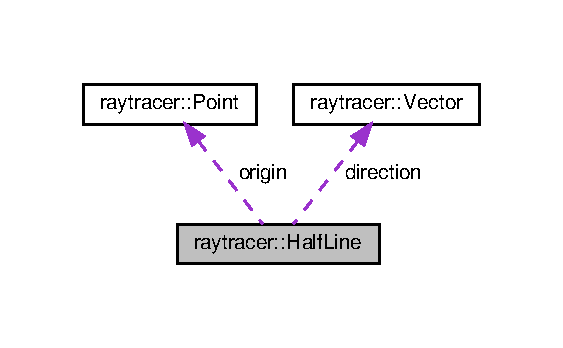
\includegraphics[width=270pt]{structraytracer_1_1HalfLine__coll__graph}
\end{center}
\end{figure}
\subsection*{Public Attributes}
\begin{DoxyCompactItemize}
\item 
\mbox{\Hypertarget{structraytracer_1_1HalfLine_a905cfe4a35c3a249af473cb348061d15}\label{structraytracer_1_1HalfLine_a905cfe4a35c3a249af473cb348061d15}} 
\hyperlink{classraytracer_1_1Point}{Point} \hyperlink{structraytracer_1_1HalfLine_a905cfe4a35c3a249af473cb348061d15}{origin}
\begin{DoxyCompactList}\small\item\em Origin. \end{DoxyCompactList}\item 
\mbox{\Hypertarget{structraytracer_1_1HalfLine_abe4077c13e9fa9706d326d9276293942}\label{structraytracer_1_1HalfLine_abe4077c13e9fa9706d326d9276293942}} 
\hyperlink{classraytracer_1_1Vector}{Vector} \hyperlink{structraytracer_1_1HalfLine_abe4077c13e9fa9706d326d9276293942}{direction}
\begin{DoxyCompactList}\small\item\em Direction. \end{DoxyCompactList}\end{DoxyCompactItemize}


\subsection{Detailed Description}
Structure representing a half line. 

It originates from a point and has a direction. 

The documentation for this struct was generated from the following file\+:\begin{DoxyCompactItemize}
\item 
/home/martin/\+C\+Lion\+Projects/raytracer/include/raytracer/geometry/Intersection.\+h\end{DoxyCompactItemize}

\hypertarget{structraytracer_1_1Intersection}{}\section{raytracer\+:\+:Intersection Struct Reference}
\label{structraytracer_1_1Intersection}\index{raytracer\+::\+Intersection@{raytracer\+::\+Intersection}}


Structure representing a single intersection of \hyperlink{classraytracer_1_1Ray}{Ray} with a \hyperlink{classraytracer_1_1Mesh}{Mesh}.  




{\ttfamily \#include $<$Ray.\+h$>$}



Collaboration diagram for raytracer\+:\+:Intersection\+:
\nopagebreak
\begin{figure}[H]
\begin{center}
\leavevmode
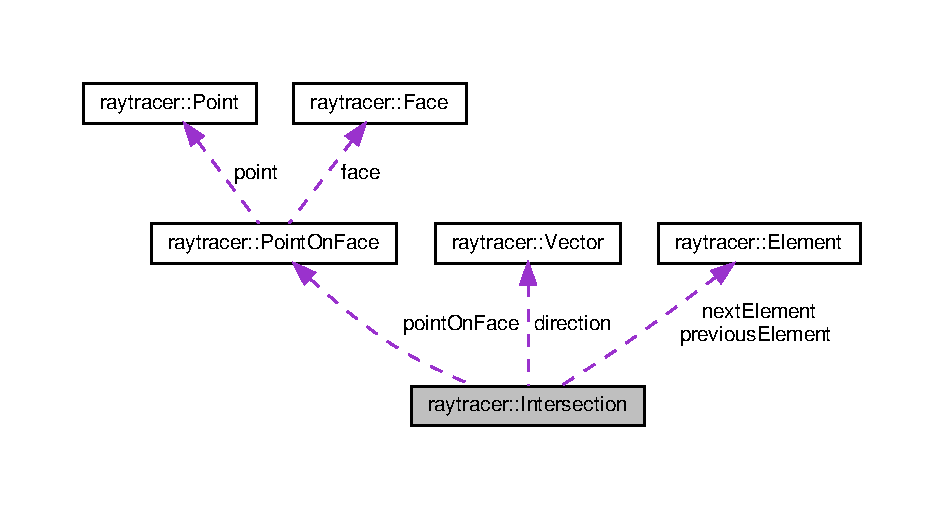
\includegraphics[width=350pt]{structraytracer_1_1Intersection__coll__graph}
\end{center}
\end{figure}
\subsection*{Public Attributes}
\begin{DoxyCompactItemize}
\item 
\mbox{\Hypertarget{structraytracer_1_1Intersection_ad63fbc92920b6ce5e0f939fba89ae0dc}\label{structraytracer_1_1Intersection_ad63fbc92920b6ce5e0f939fba89ae0dc}} 
\hyperlink{classraytracer_1_1Vector}{Vector} \hyperlink{structraytracer_1_1Intersection_ad63fbc92920b6ce5e0f939fba89ae0dc}{direction} \{\}
\begin{DoxyCompactList}\small\item\em Direction at which the \hyperlink{classraytracer_1_1Ray}{Ray} entered \hyperlink{structraytracer_1_1Intersection_afb09dd39bcd8d80373b47e36ba66fcf5}{Intersection\+::next\+Element}. \end{DoxyCompactList}\item 
\mbox{\Hypertarget{structraytracer_1_1Intersection_acd9214a1aca8b4e65008eb02a3d910fd}\label{structraytracer_1_1Intersection_acd9214a1aca8b4e65008eb02a3d910fd}} 
\hyperlink{structraytracer_1_1PointOnFace}{Point\+On\+Face} \hyperlink{structraytracer_1_1Intersection_acd9214a1aca8b4e65008eb02a3d910fd}{point\+On\+Face} \{\}
\begin{DoxyCompactList}\small\item\em \hyperlink{structraytracer_1_1PointOnFace}{Point\+On\+Face} where the \hyperlink{classraytracer_1_1Ray}{Ray} intersected the \hyperlink{classraytracer_1_1Face}{Face}. \end{DoxyCompactList}\item 
const \hyperlink{classraytracer_1_1Element}{Element} $\ast$ \hyperlink{structraytracer_1_1Intersection_afb09dd39bcd8d80373b47e36ba66fcf5}{next\+Element} \{\}
\begin{DoxyCompactList}\small\item\em Pointer to the next \hyperlink{classraytracer_1_1Element}{Element} that the ray will go to from the \hyperlink{classraytracer_1_1Face}{Face}. \end{DoxyCompactList}\item 
const \hyperlink{classraytracer_1_1Element}{Element} $\ast$ \hyperlink{structraytracer_1_1Intersection_aa4f4ef637299868b38290af358031832}{previous\+Element} \{\}
\begin{DoxyCompactList}\small\item\em Pointer to the previous \hyperlink{classraytracer_1_1Element}{Element} that the ray actually came from. \end{DoxyCompactList}\end{DoxyCompactItemize}


\subsection{Detailed Description}
Structure representing a single intersection of \hyperlink{classraytracer_1_1Ray}{Ray} with a \hyperlink{classraytracer_1_1Mesh}{Mesh}. 

\subsection{Member Data Documentation}
\mbox{\Hypertarget{structraytracer_1_1Intersection_afb09dd39bcd8d80373b47e36ba66fcf5}\label{structraytracer_1_1Intersection_afb09dd39bcd8d80373b47e36ba66fcf5}} 
\index{raytracer\+::\+Intersection@{raytracer\+::\+Intersection}!next\+Element@{next\+Element}}
\index{next\+Element@{next\+Element}!raytracer\+::\+Intersection@{raytracer\+::\+Intersection}}
\subsubsection{\texorpdfstring{next\+Element}{nextElement}}
{\footnotesize\ttfamily const \hyperlink{classraytracer_1_1Element}{Element}$\ast$ raytracer\+::\+Intersection\+::next\+Element \{\}}



Pointer to the next \hyperlink{classraytracer_1_1Element}{Element} that the ray will go to from the \hyperlink{classraytracer_1_1Face}{Face}. 

Could be null if the ray just left the \hyperlink{classraytracer_1_1Mesh}{Mesh}. \mbox{\Hypertarget{structraytracer_1_1Intersection_aa4f4ef637299868b38290af358031832}\label{structraytracer_1_1Intersection_aa4f4ef637299868b38290af358031832}} 
\index{raytracer\+::\+Intersection@{raytracer\+::\+Intersection}!previous\+Element@{previous\+Element}}
\index{previous\+Element@{previous\+Element}!raytracer\+::\+Intersection@{raytracer\+::\+Intersection}}
\subsubsection{\texorpdfstring{previous\+Element}{previousElement}}
{\footnotesize\ttfamily const \hyperlink{classraytracer_1_1Element}{Element}$\ast$ raytracer\+::\+Intersection\+::previous\+Element \{\}}



Pointer to the previous \hyperlink{classraytracer_1_1Element}{Element} that the ray actually came from. 

Could be null if the ray just entered the \hyperlink{classraytracer_1_1Mesh}{Mesh}. 

The documentation for this struct was generated from the following file\+:\begin{DoxyCompactItemize}
\item 
/home/martin/\+C\+Lion\+Projects/raytracer/include/raytracer/geometry/Ray.\+h\end{DoxyCompactItemize}

\hypertarget{classraytracer_1_1Laser}{}\section{raytracer\+:\+:Laser Class Reference}
\label{classraytracer_1_1Laser}\index{raytracer\+::\+Laser@{raytracer\+::\+Laser}}


Class representing a real physical laser.  




{\ttfamily \#include $<$Laser.\+h$>$}

\subsection*{Public Member Functions}
\begin{DoxyCompactItemize}
\item 
\hyperlink{classraytracer_1_1Laser_a141316bde09381a6f621b2df196690a0}{Laser} (\hyperlink{structraytracer_1_1Length}{Length} wavelength, Direction\+Fun direction\+Function, Energy\+Fun energy\+Function, \hyperlink{classraytracer_1_1Point}{Point} start\+Point, \hyperlink{classraytracer_1_1Point}{Point} end\+Point)
\begin{DoxyCompactList}\small\item\em Construct it using the wavelength in cm, direction\+Function, energy\+Function and two points in space between which the laser originates. \end{DoxyCompactList}\item 
void \hyperlink{classraytracer_1_1Laser_a30ab139c3170d769fffe1c2678615bf2}{generate\+Rays} (size\+\_\+t count)
\begin{DoxyCompactList}\small\item\em Generate a set of equidistant Laser\+Rays given by the parameters of the whole laser. \end{DoxyCompactList}\item 
const std\+::vector$<$ \hyperlink{classraytracer_1_1LaserRay}{Laser\+Ray} $>$ \& \hyperlink{classraytracer_1_1Laser_a1178e8800c8cd90d5274b2854c9f2fe5}{get\+Rays} () const
\begin{DoxyCompactList}\small\item\em Get all the rays in that are in the current state of \hyperlink{classraytracer_1_1Laser}{Laser}. \end{DoxyCompactList}\item 
{\footnotesize template$<$typename Direction\+Function , typename Intersection\+Function , typename Stop\+Condition $>$ }\\void \hyperlink{classraytracer_1_1Laser_a40fd2b112fb1de646861d7e93ac303e3}{generate\+Intersections} (const \hyperlink{classraytracer_1_1Mesh}{Mesh} \&mesh, Direction\+Function find\+Direction, Intersection\+Function \hyperlink{namespaceraytracer_ae44c3032cf96db5f4ba9c07f12c9a207}{find\+Intersection}, Stop\+Condition stop\+Condition)
\begin{DoxyCompactList}\small\item\em Find intersections finds all the \hyperlink{structraytracer_1_1Intersection}{Intersection} of each \hyperlink{classraytracer_1_1LaserRay}{Laser\+Ray} in \hyperlink{classraytracer_1_1Laser}{Laser} with \hyperlink{classraytracer_1_1Mesh}{Mesh}. \end{DoxyCompactList}\item 
void \hyperlink{classraytracer_1_1Laser_aeb6e2f23b0ce9b8e74eea3dc0f543345}{save\+Rays\+To\+Json} (const std\+::string \&filename)
\begin{DoxyCompactList}\small\item\em Save all the rays to a file in J\+S\+ON format. \end{DoxyCompactList}\end{DoxyCompactItemize}


\subsection{Detailed Description}
Class representing a real physical laser. 

It is given by its origin, and energy. 

\subsection{Constructor \& Destructor Documentation}
\mbox{\Hypertarget{classraytracer_1_1Laser_a141316bde09381a6f621b2df196690a0}\label{classraytracer_1_1Laser_a141316bde09381a6f621b2df196690a0}} 
\index{raytracer\+::\+Laser@{raytracer\+::\+Laser}!Laser@{Laser}}
\index{Laser@{Laser}!raytracer\+::\+Laser@{raytracer\+::\+Laser}}
\subsubsection{\texorpdfstring{Laser()}{Laser()}}
{\footnotesize\ttfamily raytracer\+::\+Laser\+::\+Laser (\begin{DoxyParamCaption}\item[{\hyperlink{structraytracer_1_1Length}{Length}}]{wavelength,  }\item[{Direction\+Fun}]{direction\+Function,  }\item[{Energy\+Fun}]{energy\+Function,  }\item[{\hyperlink{classraytracer_1_1Point}{Point}}]{start\+Point,  }\item[{\hyperlink{classraytracer_1_1Point}{Point}}]{end\+Point }\end{DoxyParamCaption})}



Construct it using the wavelength in cm, direction\+Function, energy\+Function and two points in space between which the laser originates. 

The direction\+Function should return the direction of the laser given an arbitrary point in space. The energy function should return the energy of the laser base on the parameter x. X is expected to be measured from the center of the laser.


\begin{DoxyParams}{Parameters}
{\em wavelength} & of the laser in cm \\
\hline
{\em direction\+Function} & function with signature (const \hyperlink{classraytracer_1_1Point}{Point}\& point) -\/$>$ \hyperlink{classraytracer_1_1Vector}{Vector} \\
\hline
{\em energy\+Function} & function with signature (double x) -\/$>$ double. \\
\hline
{\em start\+Point} & from which to start the generation of the rays \\
\hline
{\em end\+Point} & where to end the generation of the points \\
\hline
\end{DoxyParams}


\subsection{Member Function Documentation}
\mbox{\Hypertarget{classraytracer_1_1Laser_a40fd2b112fb1de646861d7e93ac303e3}\label{classraytracer_1_1Laser_a40fd2b112fb1de646861d7e93ac303e3}} 
\index{raytracer\+::\+Laser@{raytracer\+::\+Laser}!generate\+Intersections@{generate\+Intersections}}
\index{generate\+Intersections@{generate\+Intersections}!raytracer\+::\+Laser@{raytracer\+::\+Laser}}
\subsubsection{\texorpdfstring{generate\+Intersections()}{generateIntersections()}}
{\footnotesize\ttfamily template$<$typename Direction\+Function , typename Intersection\+Function , typename Stop\+Condition $>$ \\
void raytracer\+::\+Laser\+::generate\+Intersections (\begin{DoxyParamCaption}\item[{const \hyperlink{classraytracer_1_1Mesh}{Mesh} \&}]{mesh,  }\item[{Direction\+Function}]{find\+Direction,  }\item[{Intersection\+Function}]{find\+Intersection,  }\item[{Stop\+Condition}]{stop\+Condition }\end{DoxyParamCaption})\hspace{0.3cm}{\ttfamily [inline]}}



Find intersections finds all the \hyperlink{structraytracer_1_1Intersection}{Intersection} of each \hyperlink{classraytracer_1_1LaserRay}{Laser\+Ray} in \hyperlink{classraytracer_1_1Laser}{Laser} with \hyperlink{classraytracer_1_1Mesh}{Mesh}. 

There are multiple functional parameters to ensure high variability of this method.

\begin{DoxyNote}{Note}
{\bfseries This is the highly modular main method that is the main concern for the user.}
\end{DoxyNote}

\begin{DoxyTemplParams}{Template Parameters}
{\em Direction\+Function} & function type \\
\hline
{\em Intersection\+Function} & function type \\
\hline
{\em Stop\+Condition} & function type \\
\hline
\end{DoxyTemplParams}

\begin{DoxyParams}{Parameters}
{\em mesh} & to be intersected \\
\hline
{\em find\+Direction} & function that decides new direction every time a \hyperlink{classraytracer_1_1Face}{Face} is encountered. The function must have the following form\+: 
\begin{DoxyCode}
Vector findDirection()(
    \textcolor{keyword}{const} PointOnFace &pointOnFace,
    \textcolor{keyword}{const} Vector &previousDirection,
    \textcolor{keyword}{const} Element &previousElement,
    \textcolor{keyword}{const} Element &nextElement,
    \textcolor{keyword}{const} LaserRay &laserRay
) \{
    \textcolor{comment}{//x, y = ...}
    \textcolor{keywordflow}{return} Vector(x, y);
\}
\end{DoxyCode}
 It is recommended that you copy and paste this to implement find\+Direction. \\
\hline
{\em find\+Intersection} & function that finds the path of the \hyperlink{classraytracer_1_1Ray}{Ray} through given \hyperlink{classraytracer_1_1Element}{Element} and returns \hyperlink{structraytracer_1_1PointOnFace}{Point\+On\+Face} where the \hyperlink{classraytracer_1_1Ray}{Ray} escapes the \hyperlink{classraytracer_1_1Element}{Element}. The function mush have the following form\+: 
\begin{DoxyCode}
PointOnFace \hyperlink{namespaceraytracer_ae44c3032cf96db5f4ba9c07f12c9a207}{findIntersection}(
    \textcolor{keyword}{const} PointOnFace &entryPointOnFace,
    \textcolor{keyword}{const} Vector &entryDirection,
    \textcolor{keyword}{const} Element &element,
    \textcolor{keyword}{const} LaserRay &laserRay
) \{
    \textcolor{comment}{//point, face = ...}
    PointOnFace pointOnFace\{\};
    pointOnFace.point = point;
    pointOnFace.face = face;
    \textcolor{keywordflow}{return} pointOnFace;
\}
\end{DoxyCode}
 It is recommended that you copy and paste this to implement find\+Intersection. \\
\hline
{\em stop\+Condition} & function that returns true if the \hyperlink{classraytracer_1_1Ray}{Ray} should stop propagation. The function mush have the following form\+: 
\begin{DoxyCode}
\textcolor{keywordtype}{bool} stopCondition(
    \textcolor{keyword}{const} Element &,
    \textcolor{keyword}{const} LaserRay &laserRay
) \{
    \textcolor{comment}{//shouldStop = ...}
    \textcolor{keywordflow}{return} shouldStop;
\}
\end{DoxyCode}
 It is recommended that you copy and paste this to implement stop\+Condition. \\
\hline
\end{DoxyParams}
\mbox{\Hypertarget{classraytracer_1_1Laser_a30ab139c3170d769fffe1c2678615bf2}\label{classraytracer_1_1Laser_a30ab139c3170d769fffe1c2678615bf2}} 
\index{raytracer\+::\+Laser@{raytracer\+::\+Laser}!generate\+Rays@{generate\+Rays}}
\index{generate\+Rays@{generate\+Rays}!raytracer\+::\+Laser@{raytracer\+::\+Laser}}
\subsubsection{\texorpdfstring{generate\+Rays()}{generateRays()}}
{\footnotesize\ttfamily void raytracer\+::\+Laser\+::generate\+Rays (\begin{DoxyParamCaption}\item[{size\+\_\+t}]{count }\end{DoxyParamCaption})}



Generate a set of equidistant Laser\+Rays given by the parameters of the whole laser. 

The rays are generated originating from an edge between a start and end points of the laser. These will be set to the this \hyperlink{classraytracer_1_1Laser}{Laser} state.


\begin{DoxyParams}{Parameters}
{\em count} & number of rays to be generated \\
\hline
\end{DoxyParams}
\begin{DoxyReturn}{Returns}
a sequence of rays 
\end{DoxyReturn}
\mbox{\Hypertarget{classraytracer_1_1Laser_a1178e8800c8cd90d5274b2854c9f2fe5}\label{classraytracer_1_1Laser_a1178e8800c8cd90d5274b2854c9f2fe5}} 
\index{raytracer\+::\+Laser@{raytracer\+::\+Laser}!get\+Rays@{get\+Rays}}
\index{get\+Rays@{get\+Rays}!raytracer\+::\+Laser@{raytracer\+::\+Laser}}
\subsubsection{\texorpdfstring{get\+Rays()}{getRays()}}
{\footnotesize\ttfamily const std\+::vector$<$\hyperlink{classraytracer_1_1LaserRay}{Laser\+Ray}$>$\& raytracer\+::\+Laser\+::get\+Rays (\begin{DoxyParamCaption}{ }\end{DoxyParamCaption}) const}



Get all the rays in that are in the current state of \hyperlink{classraytracer_1_1Laser}{Laser}. 

\begin{DoxyReturn}{Returns}
all rays 
\end{DoxyReturn}
\mbox{\Hypertarget{classraytracer_1_1Laser_aeb6e2f23b0ce9b8e74eea3dc0f543345}\label{classraytracer_1_1Laser_aeb6e2f23b0ce9b8e74eea3dc0f543345}} 
\index{raytracer\+::\+Laser@{raytracer\+::\+Laser}!save\+Rays\+To\+Json@{save\+Rays\+To\+Json}}
\index{save\+Rays\+To\+Json@{save\+Rays\+To\+Json}!raytracer\+::\+Laser@{raytracer\+::\+Laser}}
\subsubsection{\texorpdfstring{save\+Rays\+To\+Json()}{saveRaysToJson()}}
{\footnotesize\ttfamily void raytracer\+::\+Laser\+::save\+Rays\+To\+Json (\begin{DoxyParamCaption}\item[{const std\+::string \&}]{filename }\end{DoxyParamCaption})}



Save all the rays to a file in J\+S\+ON format. 

There will be one object called rays. It is an array of rays each being a sequence of points eg. (0, 1) 
\begin{DoxyParams}{Parameters}
{\em filename} & name of the json file including extension \\
\hline
\end{DoxyParams}


The documentation for this class was generated from the following file\+:\begin{DoxyCompactItemize}
\item 
/home/martin/\+C\+Lion\+Projects/raytracer/include/raytracer/physics/Laser.\+h\end{DoxyCompactItemize}

\hypertarget{classraytracer_1_1LaserRay}{}\section{raytracer\+:\+:Laser\+Ray Class Reference}
\label{classraytracer_1_1LaserRay}\index{raytracer\+::\+Laser\+Ray@{raytracer\+::\+Laser\+Ray}}


Class representing a single \hyperlink{classraytracer_1_1LaserRay}{Laser\+Ray}.  




{\ttfamily \#include $<$Laser\+Ray.\+h$>$}



Collaboration diagram for raytracer\+:\+:Laser\+Ray\+:
\nopagebreak
\begin{figure}[H]
\begin{center}
\leavevmode
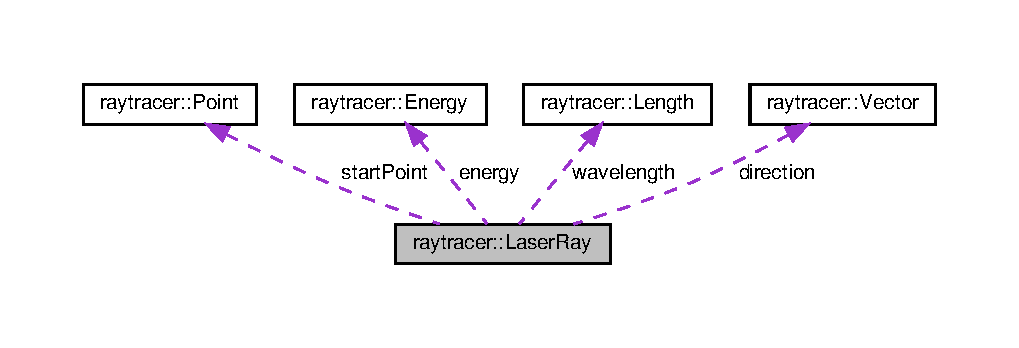
\includegraphics[width=350pt]{classraytracer_1_1LaserRay__coll__graph}
\end{center}
\end{figure}
\subsection*{Public Member Functions}
\begin{DoxyCompactItemize}
\item 
\mbox{\Hypertarget{classraytracer_1_1LaserRay_ac7ca600dec49c7d782e18bbba144e483}\label{classraytracer_1_1LaserRay_ac7ca600dec49c7d782e18bbba144e483}} 
\hyperlink{structraytracer_1_1Density}{Density} \hyperlink{classraytracer_1_1LaserRay_ac7ca600dec49c7d782e18bbba144e483}{get\+Critical\+Density} () const
\begin{DoxyCompactList}\small\item\em The electron critical density of the \hyperlink{classraytracer_1_1LaserRay}{Laser\+Ray}. \end{DoxyCompactList}\item 
double \hyperlink{classraytracer_1_1LaserRay_af841f0b8279f67242414c1709ce61212}{get\+Refractive\+Index} (const \hyperlink{structraytracer_1_1Density}{Density} \&density, const \hyperlink{structraytracer_1_1Frequency}{Frequency} \&collision\+Frequency) const
\begin{DoxyCompactList}\small\item\em Calculate the index of refraction based on current density, collisional frequency. \end{DoxyCompactList}\item 
double \hyperlink{classraytracer_1_1LaserRay_a9b73d2d5488310646ad750243f5e6b13}{get\+Inverse\+Bremsstrahlung\+Coeff} (const \hyperlink{structraytracer_1_1Density}{Density} \&density, const \hyperlink{structraytracer_1_1Frequency}{Frequency} \&collision\+Frequency) const
\begin{DoxyCompactList}\small\item\em Calculate the inverse bremsstrahlung coefficient base on current density and collisional frequency. \end{DoxyCompactList}\item 
std\+::complex$<$ double $>$ \hyperlink{classraytracer_1_1LaserRay_a7ab8b571769cf7bd6d9d71694db025aa}{get\+Permittivity} (const \hyperlink{structraytracer_1_1Density}{Density} \&density, const \hyperlink{structraytracer_1_1Frequency}{Frequency} \&collision\+Frequency) const
\begin{DoxyCompactList}\small\item\em Calculate the permittivity based on current density and collision\+Frequency. \end{DoxyCompactList}\item 
{\footnotesize template$<$typename Direction\+Function , typename Intersection\+Function , typename Stop\+Condition $>$ }\\void \hyperlink{classraytracer_1_1LaserRay_a50a1b65c99c56fe6eb7fd89e01f84acf}{generate\+Intersections} (const \hyperlink{classraytracer_1_1Mesh}{Mesh} \&mesh, Direction\+Function find\+Direction, Intersection\+Function \hyperlink{namespaceraytracer_ae44c3032cf96db5f4ba9c07f12c9a207}{find\+Intersection}, Stop\+Condition stop\+Condition)
\begin{DoxyCompactList}\small\item\em Wrapper around \hyperlink{classraytracer_1_1Ray_a9ebcb3641ec730e5b94452833b69c68d}{Ray\+::find\+Intersections()}. \end{DoxyCompactList}\end{DoxyCompactItemize}
\subsection*{Public Attributes}
\begin{DoxyCompactItemize}
\item 
\hyperlink{classraytracer_1_1Point}{Point} \hyperlink{classraytracer_1_1LaserRay_a6970072ba9bbe9a958d9595386d39cc9}{start\+Point} \{\}
\begin{DoxyCompactList}\small\item\em The point from which the \hyperlink{classraytracer_1_1LaserRay}{Laser\+Ray} originates. \end{DoxyCompactList}\item 
\hyperlink{classraytracer_1_1Vector}{Vector} \hyperlink{classraytracer_1_1LaserRay_af50d079eead68440a707dfe63b2029d8}{direction} \{\}
\begin{DoxyCompactList}\small\item\em The initial direction of the \hyperlink{classraytracer_1_1LaserRay}{Laser\+Ray}. \end{DoxyCompactList}\item 
\hyperlink{structraytracer_1_1Energy}{Energy} \hyperlink{classraytracer_1_1LaserRay_a5434b2b8f9c1e5c695761e4c1147b00e}{energy} \{\}
\begin{DoxyCompactList}\small\item\em Absolute energy carried by the \hyperlink{classraytracer_1_1LaserRay}{Laser\+Ray}. \end{DoxyCompactList}\item 
\mbox{\Hypertarget{classraytracer_1_1LaserRay_ae3b24463ade2202eb37972eb1cdb88e0}\label{classraytracer_1_1LaserRay_ae3b24463ade2202eb37972eb1cdb88e0}} 
\hyperlink{structraytracer_1_1Length}{Length} \hyperlink{classraytracer_1_1LaserRay_ae3b24463ade2202eb37972eb1cdb88e0}{wavelength} \{\}
\begin{DoxyCompactList}\small\item\em Wavelength of the \hyperlink{classraytracer_1_1LaserRay}{Laser\+Ray} in cm. \end{DoxyCompactList}\item 
std\+::vector$<$ \hyperlink{structraytracer_1_1Intersection}{Intersection} $>$ \hyperlink{classraytracer_1_1LaserRay_a2f15a3a20e496fdc6308d62d0a520bfd}{intersections}
\begin{DoxyCompactList}\small\item\em Sequence of all intersections with given \hyperlink{classraytracer_1_1Mesh}{Mesh}. \end{DoxyCompactList}\end{DoxyCompactItemize}


\subsection{Detailed Description}
Class representing a single \hyperlink{classraytracer_1_1LaserRay}{Laser\+Ray}. 

It has associated energy but no width for now. 

\subsection{Member Function Documentation}
\mbox{\Hypertarget{classraytracer_1_1LaserRay_a50a1b65c99c56fe6eb7fd89e01f84acf}\label{classraytracer_1_1LaserRay_a50a1b65c99c56fe6eb7fd89e01f84acf}} 
\index{raytracer\+::\+Laser\+Ray@{raytracer\+::\+Laser\+Ray}!generate\+Intersections@{generate\+Intersections}}
\index{generate\+Intersections@{generate\+Intersections}!raytracer\+::\+Laser\+Ray@{raytracer\+::\+Laser\+Ray}}
\subsubsection{\texorpdfstring{generate\+Intersections()}{generateIntersections()}}
{\footnotesize\ttfamily template$<$typename Direction\+Function , typename Intersection\+Function , typename Stop\+Condition $>$ \\
void raytracer\+::\+Laser\+Ray\+::generate\+Intersections (\begin{DoxyParamCaption}\item[{const \hyperlink{classraytracer_1_1Mesh}{Mesh} \&}]{mesh,  }\item[{Direction\+Function}]{find\+Direction,  }\item[{Intersection\+Function}]{find\+Intersection,  }\item[{Stop\+Condition}]{stop\+Condition }\end{DoxyParamCaption})\hspace{0.3cm}{\ttfamily [inline]}}



Wrapper around \hyperlink{classraytracer_1_1Ray_a9ebcb3641ec730e5b94452833b69c68d}{Ray\+::find\+Intersections()}. 

It generates a ray based on the \hyperlink{classraytracer_1_1LaserRay}{Laser\+Ray} properties and saves the result to \hyperlink{classraytracer_1_1LaserRay_a2f15a3a20e496fdc6308d62d0a520bfd}{Laser\+Ray\+::intersections}.


\begin{DoxyTemplParams}{Template Parameters}
{\em Intersection\+Function} & \\
\hline
{\em Stop\+Condition} & \\
\hline
\end{DoxyTemplParams}

\begin{DoxyParams}{Parameters}
{\em mesh} & to be intersected \\
\hline
{\em find\+Direction} & will be propagated to \hyperlink{classraytracer_1_1Ray_a9ebcb3641ec730e5b94452833b69c68d}{Ray\+::find\+Intersections()} as is. \\
\hline
{\em find\+Intersection} & will be propagated to \hyperlink{classraytracer_1_1Ray_a9ebcb3641ec730e5b94452833b69c68d}{Ray\+::find\+Intersections()} as is. \\
\hline
{\em stop\+Condition} & will be propagated to \hyperlink{classraytracer_1_1Ray_a9ebcb3641ec730e5b94452833b69c68d}{Ray\+::find\+Intersections()} as is. \\
\hline
\end{DoxyParams}
\mbox{\Hypertarget{classraytracer_1_1LaserRay_a9b73d2d5488310646ad750243f5e6b13}\label{classraytracer_1_1LaserRay_a9b73d2d5488310646ad750243f5e6b13}} 
\index{raytracer\+::\+Laser\+Ray@{raytracer\+::\+Laser\+Ray}!get\+Inverse\+Bremsstrahlung\+Coeff@{get\+Inverse\+Bremsstrahlung\+Coeff}}
\index{get\+Inverse\+Bremsstrahlung\+Coeff@{get\+Inverse\+Bremsstrahlung\+Coeff}!raytracer\+::\+Laser\+Ray@{raytracer\+::\+Laser\+Ray}}
\subsubsection{\texorpdfstring{get\+Inverse\+Bremsstrahlung\+Coeff()}{getInverseBremsstrahlungCoeff()}}
{\footnotesize\ttfamily double raytracer\+::\+Laser\+Ray\+::get\+Inverse\+Bremsstrahlung\+Coeff (\begin{DoxyParamCaption}\item[{const \hyperlink{structraytracer_1_1Density}{Density} \&}]{density,  }\item[{const \hyperlink{structraytracer_1_1Frequency}{Frequency} \&}]{collision\+Frequency }\end{DoxyParamCaption}) const\hspace{0.3cm}{\ttfamily [inline]}}



Calculate the inverse bremsstrahlung coefficient base on current density and collisional frequency. 


\begin{DoxyParams}{Parameters}
{\em density} & \\
\hline
{\em collision\+Frequency} & \\
\hline
\end{DoxyParams}
\begin{DoxyReturn}{Returns}

\end{DoxyReturn}
\mbox{\Hypertarget{classraytracer_1_1LaserRay_a7ab8b571769cf7bd6d9d71694db025aa}\label{classraytracer_1_1LaserRay_a7ab8b571769cf7bd6d9d71694db025aa}} 
\index{raytracer\+::\+Laser\+Ray@{raytracer\+::\+Laser\+Ray}!get\+Permittivity@{get\+Permittivity}}
\index{get\+Permittivity@{get\+Permittivity}!raytracer\+::\+Laser\+Ray@{raytracer\+::\+Laser\+Ray}}
\subsubsection{\texorpdfstring{get\+Permittivity()}{getPermittivity()}}
{\footnotesize\ttfamily std\+::complex$<$double$>$ raytracer\+::\+Laser\+Ray\+::get\+Permittivity (\begin{DoxyParamCaption}\item[{const \hyperlink{structraytracer_1_1Density}{Density} \&}]{density,  }\item[{const \hyperlink{structraytracer_1_1Frequency}{Frequency} \&}]{collision\+Frequency }\end{DoxyParamCaption}) const\hspace{0.3cm}{\ttfamily [inline]}}



Calculate the permittivity based on current density and collision\+Frequency. 


\begin{DoxyParams}{Parameters}
{\em density} & \\
\hline
{\em collision\+Frequency} & \\
\hline
\end{DoxyParams}
\begin{DoxyReturn}{Returns}
permittivity 
\end{DoxyReturn}
\mbox{\Hypertarget{classraytracer_1_1LaserRay_af841f0b8279f67242414c1709ce61212}\label{classraytracer_1_1LaserRay_af841f0b8279f67242414c1709ce61212}} 
\index{raytracer\+::\+Laser\+Ray@{raytracer\+::\+Laser\+Ray}!get\+Refractive\+Index@{get\+Refractive\+Index}}
\index{get\+Refractive\+Index@{get\+Refractive\+Index}!raytracer\+::\+Laser\+Ray@{raytracer\+::\+Laser\+Ray}}
\subsubsection{\texorpdfstring{get\+Refractive\+Index()}{getRefractiveIndex()}}
{\footnotesize\ttfamily double raytracer\+::\+Laser\+Ray\+::get\+Refractive\+Index (\begin{DoxyParamCaption}\item[{const \hyperlink{structraytracer_1_1Density}{Density} \&}]{density,  }\item[{const \hyperlink{structraytracer_1_1Frequency}{Frequency} \&}]{collision\+Frequency }\end{DoxyParamCaption}) const}



Calculate the index of refraction based on current density, collisional frequency. 


\begin{DoxyParams}{Parameters}
{\em density} & at which the refractive index is to be calculated \\
\hline
{\em collision\+Frequency} & current collisional frequency \\
\hline
\end{DoxyParams}
\begin{DoxyReturn}{Returns}
refractive index 
\end{DoxyReturn}


\subsection{Member Data Documentation}
\mbox{\Hypertarget{classraytracer_1_1LaserRay_af50d079eead68440a707dfe63b2029d8}\label{classraytracer_1_1LaserRay_af50d079eead68440a707dfe63b2029d8}} 
\index{raytracer\+::\+Laser\+Ray@{raytracer\+::\+Laser\+Ray}!direction@{direction}}
\index{direction@{direction}!raytracer\+::\+Laser\+Ray@{raytracer\+::\+Laser\+Ray}}
\subsubsection{\texorpdfstring{direction}{direction}}
{\footnotesize\ttfamily \hyperlink{classraytracer_1_1Vector}{Vector} raytracer\+::\+Laser\+Ray\+::direction \{\}}



The initial direction of the \hyperlink{classraytracer_1_1LaserRay}{Laser\+Ray}. 

\mbox{\Hypertarget{classraytracer_1_1LaserRay_a5434b2b8f9c1e5c695761e4c1147b00e}\label{classraytracer_1_1LaserRay_a5434b2b8f9c1e5c695761e4c1147b00e}} 
\index{raytracer\+::\+Laser\+Ray@{raytracer\+::\+Laser\+Ray}!energy@{energy}}
\index{energy@{energy}!raytracer\+::\+Laser\+Ray@{raytracer\+::\+Laser\+Ray}}
\subsubsection{\texorpdfstring{energy}{energy}}
{\footnotesize\ttfamily \hyperlink{structraytracer_1_1Energy}{Energy} raytracer\+::\+Laser\+Ray\+::energy \{\}}



Absolute energy carried by the \hyperlink{classraytracer_1_1LaserRay}{Laser\+Ray}. 

\mbox{\Hypertarget{classraytracer_1_1LaserRay_a2f15a3a20e496fdc6308d62d0a520bfd}\label{classraytracer_1_1LaserRay_a2f15a3a20e496fdc6308d62d0a520bfd}} 
\index{raytracer\+::\+Laser\+Ray@{raytracer\+::\+Laser\+Ray}!intersections@{intersections}}
\index{intersections@{intersections}!raytracer\+::\+Laser\+Ray@{raytracer\+::\+Laser\+Ray}}
\subsubsection{\texorpdfstring{intersections}{intersections}}
{\footnotesize\ttfamily std\+::vector$<$\hyperlink{structraytracer_1_1Intersection}{Intersection}$>$ raytracer\+::\+Laser\+Ray\+::intersections}



Sequence of all intersections with given \hyperlink{classraytracer_1_1Mesh}{Mesh}. 

This is empty if no generate\+Intersections was called. \mbox{\Hypertarget{classraytracer_1_1LaserRay_a6970072ba9bbe9a958d9595386d39cc9}\label{classraytracer_1_1LaserRay_a6970072ba9bbe9a958d9595386d39cc9}} 
\index{raytracer\+::\+Laser\+Ray@{raytracer\+::\+Laser\+Ray}!start\+Point@{start\+Point}}
\index{start\+Point@{start\+Point}!raytracer\+::\+Laser\+Ray@{raytracer\+::\+Laser\+Ray}}
\subsubsection{\texorpdfstring{start\+Point}{startPoint}}
{\footnotesize\ttfamily \hyperlink{classraytracer_1_1Point}{Point} raytracer\+::\+Laser\+Ray\+::start\+Point \{\}}



The point from which the \hyperlink{classraytracer_1_1LaserRay}{Laser\+Ray} originates. 



The documentation for this class was generated from the following file\+:\begin{DoxyCompactItemize}
\item 
/home/martin/\+C\+Lion\+Projects/raytracer/include/raytracer/physics/Laser\+Ray.\+h\end{DoxyCompactItemize}

\hypertarget{structraytracer_1_1Length}{}\section{raytracer\+:\+:Length Struct Reference}
\label{structraytracer_1_1Length}\index{raytracer\+::\+Length@{raytracer\+::\+Length}}


Strong type representing length in cm.  




{\ttfamily \#include $<$Magnitudes.\+h$>$}



\subsection{Detailed Description}
Strong type representing length in cm. 



The documentation for this struct was generated from the following file\+:\begin{DoxyCompactItemize}
\item 
/home/martin/\+C\+Lion\+Projects/raytracer/include/raytracer/physics/Magnitudes.\+h\end{DoxyCompactItemize}

\hypertarget{classraytracer_1_1Mesh}{}\section{raytracer\+:\+:Mesh Class Reference}
\label{classraytracer_1_1Mesh}\index{raytracer\+::\+Mesh@{raytracer\+::\+Mesh}}


Class representing a mesh (2D for now).  




{\ttfamily \#include $<$Mesh.\+h$>$}

\subsection*{Public Member Functions}
\begin{DoxyCompactItemize}
\item 
\mbox{\Hypertarget{classraytracer_1_1Mesh_ad009fe99caff6e954dd237c3d62a3dc1}\label{classraytracer_1_1Mesh_ad009fe99caff6e954dd237c3d62a3dc1}} 
\hyperlink{classraytracer_1_1Mesh_ad009fe99caff6e954dd237c3d62a3dc1}{Mesh} (mfem\+::\+Mesh $\ast$mesh)
\begin{DoxyCompactList}\small\item\em Create a rectangular mesh given. \end{DoxyCompactList}\item 
\hyperlink{classraytracer_1_1Element}{Element} $\ast$ \hyperlink{classraytracer_1_1Mesh_a37bb91c21c404e4ff4432d7169918c38}{get\+Face\+Adjacent\+Element} (const \hyperlink{classraytracer_1_1Face}{Face} $\ast$face, const \hyperlink{classraytracer_1_1Vector}{Vector} \&direction) const
\begin{DoxyCompactList}\small\item\em Given a \hyperlink{classraytracer_1_1Face}{Face} return the adjacent \hyperlink{classraytracer_1_1Element}{Element} to this face in given direction. \end{DoxyCompactList}\item 
std\+::vector$<$ \hyperlink{classraytracer_1_1Face}{Face} $\ast$ $>$ \hyperlink{classraytracer_1_1Mesh_a4f2718e871ca63809445b33b56fa02de}{get\+Boundary} () const
\begin{DoxyCompactList}\small\item\em Return a sequence of faces that are on the mesh boundary. \end{DoxyCompactList}\end{DoxyCompactItemize}


\subsection{Detailed Description}
Class representing a mesh (2D for now). 

It encapsulates the class mfem\+::\+Mesh and provides some convenience methods. 

\subsection{Member Function Documentation}
\mbox{\Hypertarget{classraytracer_1_1Mesh_a4f2718e871ca63809445b33b56fa02de}\label{classraytracer_1_1Mesh_a4f2718e871ca63809445b33b56fa02de}} 
\index{raytracer\+::\+Mesh@{raytracer\+::\+Mesh}!get\+Boundary@{get\+Boundary}}
\index{get\+Boundary@{get\+Boundary}!raytracer\+::\+Mesh@{raytracer\+::\+Mesh}}
\subsubsection{\texorpdfstring{get\+Boundary()}{getBoundary()}}
{\footnotesize\ttfamily std\+::vector$<$\hyperlink{classraytracer_1_1Face}{Face} $\ast$$>$ raytracer\+::\+Mesh\+::get\+Boundary (\begin{DoxyParamCaption}{ }\end{DoxyParamCaption}) const}



Return a sequence of faces that are on the mesh boundary. 

\begin{DoxyReturn}{Returns}
sequence of faces. 
\end{DoxyReturn}
\mbox{\Hypertarget{classraytracer_1_1Mesh_a37bb91c21c404e4ff4432d7169918c38}\label{classraytracer_1_1Mesh_a37bb91c21c404e4ff4432d7169918c38}} 
\index{raytracer\+::\+Mesh@{raytracer\+::\+Mesh}!get\+Face\+Adjacent\+Element@{get\+Face\+Adjacent\+Element}}
\index{get\+Face\+Adjacent\+Element@{get\+Face\+Adjacent\+Element}!raytracer\+::\+Mesh@{raytracer\+::\+Mesh}}
\subsubsection{\texorpdfstring{get\+Face\+Adjacent\+Element()}{getFaceAdjacentElement()}}
{\footnotesize\ttfamily \hyperlink{classraytracer_1_1Element}{Element}$\ast$ raytracer\+::\+Mesh\+::get\+Face\+Adjacent\+Element (\begin{DoxyParamCaption}\item[{const \hyperlink{classraytracer_1_1Face}{Face} $\ast$}]{face,  }\item[{const \hyperlink{classraytracer_1_1Vector}{Vector} \&}]{direction }\end{DoxyParamCaption}) const}



Given a \hyperlink{classraytracer_1_1Face}{Face} return the adjacent \hyperlink{classraytracer_1_1Element}{Element} to this face in given direction. 

It is expected that there are two or less elements adjacent to the face. If there is no element adjacent in given direction, nullptr is returned.


\begin{DoxyParams}{Parameters}
{\em face} & whose adjacent elements are to be found. \\
\hline
{\em direction} & in which to search for elements. \\
\hline
\end{DoxyParams}
\begin{DoxyReturn}{Returns}
The \hyperlink{classraytracer_1_1Element}{Element} pointer if found or nullptr if not. 
\end{DoxyReturn}


The documentation for this class was generated from the following file\+:\begin{DoxyCompactItemize}
\item 
/home/martin/\+C\+Lion\+Projects/raytracer/include/raytracer/geometry/Mesh.\+h\end{DoxyCompactItemize}

\hypertarget{classraytracer_1_1MeshFunction}{}\section{raytracer\+:\+:Mesh\+Function Class Reference}
\label{classraytracer_1_1MeshFunction}\index{raytracer\+::\+Mesh\+Function@{raytracer\+::\+Mesh\+Function}}


Abstract interface.  




{\ttfamily \#include $<$Mesh\+Function.\+h$>$}



Inheritance diagram for raytracer\+:\+:Mesh\+Function\+:
\nopagebreak
\begin{figure}[H]
\begin{center}
\leavevmode
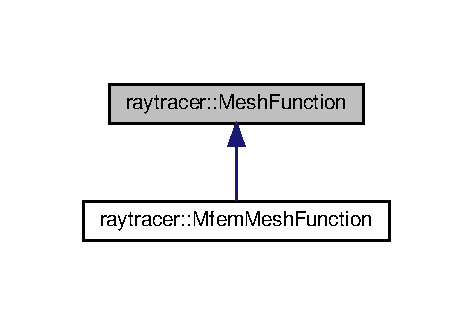
\includegraphics[width=227pt]{classraytracer_1_1MeshFunction__inherit__graph}
\end{center}
\end{figure}
\subsection*{Public Member Functions}
\begin{DoxyCompactItemize}
\item 
virtual double \hyperlink{classraytracer_1_1MeshFunction_a49888c1924a473a1d98564a4732edd3a}{get\+Value} (const \hyperlink{classraytracer_1_1Element}{Element} \&) const =0
\begin{DoxyCompactList}\small\item\em Override this. \end{DoxyCompactList}\item 
virtual void \hyperlink{classraytracer_1_1MeshFunction_a0d71fc5b456edd7a89267a071ae6dd81}{set\+Value} (const \hyperlink{classraytracer_1_1Element}{Element} \&, double value)=0
\begin{DoxyCompactList}\small\item\em Override this. \end{DoxyCompactList}\item 
virtual void \hyperlink{classraytracer_1_1MeshFunction_a134b7ca4400d04030a67cadd691ee879}{add\+Value} (const \hyperlink{classraytracer_1_1Element}{Element} \&, double value)=0
\begin{DoxyCompactList}\small\item\em Override this. \end{DoxyCompactList}\end{DoxyCompactItemize}


\subsection{Detailed Description}
Abstract interface. 

To obey this \hyperlink{classraytracer_1_1MeshFunction}{Mesh\+Function} interface get\+Value, set\+Value and add\+Value methods must be implemented. 

\subsection{Member Function Documentation}
\mbox{\Hypertarget{classraytracer_1_1MeshFunction_a134b7ca4400d04030a67cadd691ee879}\label{classraytracer_1_1MeshFunction_a134b7ca4400d04030a67cadd691ee879}} 
\index{raytracer\+::\+Mesh\+Function@{raytracer\+::\+Mesh\+Function}!add\+Value@{add\+Value}}
\index{add\+Value@{add\+Value}!raytracer\+::\+Mesh\+Function@{raytracer\+::\+Mesh\+Function}}
\subsubsection{\texorpdfstring{add\+Value()}{addValue()}}
{\footnotesize\ttfamily virtual void raytracer\+::\+Mesh\+Function\+::add\+Value (\begin{DoxyParamCaption}\item[{const \hyperlink{classraytracer_1_1Element}{Element} \&}]{,  }\item[{double}]{value }\end{DoxyParamCaption})\hspace{0.3cm}{\ttfamily [pure virtual]}}



Override this. 


\begin{DoxyParams}{Parameters}
{\em value} & to be added to current value at element. \\
\hline
\end{DoxyParams}


Implemented in \hyperlink{classraytracer_1_1MfemMeshFunction_a1c9f0ec943afb1d069ddeb85ee9bb2c8}{raytracer\+::\+Mfem\+Mesh\+Function}.

\mbox{\Hypertarget{classraytracer_1_1MeshFunction_a49888c1924a473a1d98564a4732edd3a}\label{classraytracer_1_1MeshFunction_a49888c1924a473a1d98564a4732edd3a}} 
\index{raytracer\+::\+Mesh\+Function@{raytracer\+::\+Mesh\+Function}!get\+Value@{get\+Value}}
\index{get\+Value@{get\+Value}!raytracer\+::\+Mesh\+Function@{raytracer\+::\+Mesh\+Function}}
\subsubsection{\texorpdfstring{get\+Value()}{getValue()}}
{\footnotesize\ttfamily virtual double raytracer\+::\+Mesh\+Function\+::get\+Value (\begin{DoxyParamCaption}\item[{const \hyperlink{classraytracer_1_1Element}{Element} \&}]{ }\end{DoxyParamCaption}) const\hspace{0.3cm}{\ttfamily [pure virtual]}}



Override this. 

\begin{DoxyReturn}{Returns}
value of \hyperlink{classraytracer_1_1MeshFunction}{Mesh\+Function} at element 
\end{DoxyReturn}


Implemented in \hyperlink{classraytracer_1_1MfemMeshFunction_a3e7183c2cca55df6115176d1d9030846}{raytracer\+::\+Mfem\+Mesh\+Function}.

\mbox{\Hypertarget{classraytracer_1_1MeshFunction_a0d71fc5b456edd7a89267a071ae6dd81}\label{classraytracer_1_1MeshFunction_a0d71fc5b456edd7a89267a071ae6dd81}} 
\index{raytracer\+::\+Mesh\+Function@{raytracer\+::\+Mesh\+Function}!set\+Value@{set\+Value}}
\index{set\+Value@{set\+Value}!raytracer\+::\+Mesh\+Function@{raytracer\+::\+Mesh\+Function}}
\subsubsection{\texorpdfstring{set\+Value()}{setValue()}}
{\footnotesize\ttfamily virtual void raytracer\+::\+Mesh\+Function\+::set\+Value (\begin{DoxyParamCaption}\item[{const \hyperlink{classraytracer_1_1Element}{Element} \&}]{,  }\item[{double}]{value }\end{DoxyParamCaption})\hspace{0.3cm}{\ttfamily [pure virtual]}}



Override this. 


\begin{DoxyParams}{Parameters}
{\em value} & value to be set at element \\
\hline
\end{DoxyParams}


Implemented in \hyperlink{classraytracer_1_1MfemMeshFunction_aa7c06ea3f585a45573174b073da58ee1}{raytracer\+::\+Mfem\+Mesh\+Function}.



The documentation for this class was generated from the following file\+:\begin{DoxyCompactItemize}
\item 
/home/martin/\+C\+Lion\+Projects/raytracer/include/raytracer/geometry/Mesh\+Function.\+h\end{DoxyCompactItemize}

\hypertarget{classraytracer_1_1MfemMeshFunction}{}\section{raytracer\+:\+:Mfem\+Mesh\+Function Class Reference}
\label{classraytracer_1_1MfemMeshFunction}\index{raytracer\+::\+Mfem\+Mesh\+Function@{raytracer\+::\+Mfem\+Mesh\+Function}}


Discrete function what has constant values at \hyperlink{classraytracer_1_1Mesh}{Mesh} elements.  




{\ttfamily \#include $<$Mesh\+Function.\+h$>$}



Inheritance diagram for raytracer\+:\+:Mfem\+Mesh\+Function\+:
\nopagebreak
\begin{figure}[H]
\begin{center}
\leavevmode
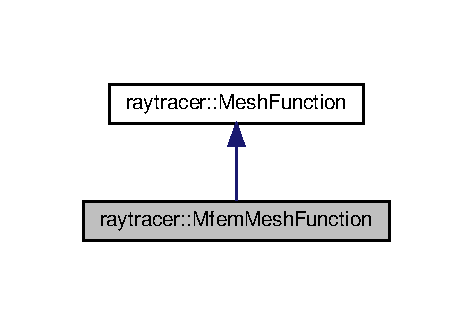
\includegraphics[width=227pt]{classraytracer_1_1MfemMeshFunction__inherit__graph}
\end{center}
\end{figure}


Collaboration diagram for raytracer\+:\+:Mfem\+Mesh\+Function\+:
\nopagebreak
\begin{figure}[H]
\begin{center}
\leavevmode
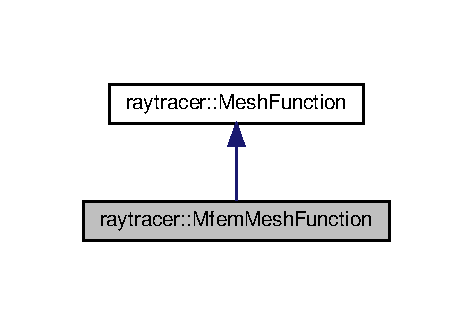
\includegraphics[width=227pt]{classraytracer_1_1MfemMeshFunction__coll__graph}
\end{center}
\end{figure}
\subsection*{Public Member Functions}
\begin{DoxyCompactItemize}
\item 
\hyperlink{classraytracer_1_1MfemMeshFunction_a92a9d86fa4b15e3514e15ad50d534bf6}{Mfem\+Mesh\+Function} (mfem\+::\+Grid\+Function \&grid\+Function, const mfem\+::\+Finite\+Element\+Space \&finite\+Element\+Space)
\begin{DoxyCompactList}\small\item\em Create the \hyperlink{classraytracer_1_1MeshFunction}{Mesh\+Function} from a mfem\+::\+Grid\+Function and mfem\+::\+Finite\+Element\+Space. \end{DoxyCompactList}\item 
double \hyperlink{classraytracer_1_1MfemMeshFunction_a3e7183c2cca55df6115176d1d9030846}{get\+Value} (const \hyperlink{classraytracer_1_1Element}{Element} \&element) const override
\begin{DoxyCompactList}\small\item\em Get a value at \hyperlink{classraytracer_1_1Element}{Element}. \end{DoxyCompactList}\item 
void \hyperlink{classraytracer_1_1MfemMeshFunction_aa7c06ea3f585a45573174b073da58ee1}{set\+Value} (const \hyperlink{classraytracer_1_1Element}{Element} \&element, double value) override
\begin{DoxyCompactList}\small\item\em Set a value at \hyperlink{classraytracer_1_1Element}{Element}. \end{DoxyCompactList}\item 
void \hyperlink{classraytracer_1_1MfemMeshFunction_a1c9f0ec943afb1d069ddeb85ee9bb2c8}{add\+Value} (const \hyperlink{classraytracer_1_1Element}{Element} \&element, double value) override
\begin{DoxyCompactList}\small\item\em Add a value to existing value at \hyperlink{classraytracer_1_1Element}{Element}. \end{DoxyCompactList}\end{DoxyCompactItemize}


\subsection{Detailed Description}
Discrete function what has constant values at \hyperlink{classraytracer_1_1Mesh}{Mesh} elements. 

Provides a way to query the Grid\+Function given an element. 

\subsection{Constructor \& Destructor Documentation}
\mbox{\Hypertarget{classraytracer_1_1MfemMeshFunction_a92a9d86fa4b15e3514e15ad50d534bf6}\label{classraytracer_1_1MfemMeshFunction_a92a9d86fa4b15e3514e15ad50d534bf6}} 
\index{raytracer\+::\+Mfem\+Mesh\+Function@{raytracer\+::\+Mfem\+Mesh\+Function}!Mfem\+Mesh\+Function@{Mfem\+Mesh\+Function}}
\index{Mfem\+Mesh\+Function@{Mfem\+Mesh\+Function}!raytracer\+::\+Mfem\+Mesh\+Function@{raytracer\+::\+Mfem\+Mesh\+Function}}
\subsubsection{\texorpdfstring{Mfem\+Mesh\+Function()}{MfemMeshFunction()}}
{\footnotesize\ttfamily raytracer\+::\+Mfem\+Mesh\+Function\+::\+Mfem\+Mesh\+Function (\begin{DoxyParamCaption}\item[{mfem\+::\+Grid\+Function \&}]{grid\+Function,  }\item[{const mfem\+::\+Finite\+Element\+Space \&}]{finite\+Element\+Space }\end{DoxyParamCaption})\hspace{0.3cm}{\ttfamily [explicit]}}



Create the \hyperlink{classraytracer_1_1MeshFunction}{Mesh\+Function} from a mfem\+::\+Grid\+Function and mfem\+::\+Finite\+Element\+Space. 


\begin{DoxyParams}{Parameters}
{\em grid\+Function} & a mutable reference will be kept. \\
\hline
{\em finite\+Element\+Space} & const reference will be kept -\/ caution\+: L2 space is expected! \\
\hline
\end{DoxyParams}


\subsection{Member Function Documentation}
\mbox{\Hypertarget{classraytracer_1_1MfemMeshFunction_a1c9f0ec943afb1d069ddeb85ee9bb2c8}\label{classraytracer_1_1MfemMeshFunction_a1c9f0ec943afb1d069ddeb85ee9bb2c8}} 
\index{raytracer\+::\+Mfem\+Mesh\+Function@{raytracer\+::\+Mfem\+Mesh\+Function}!add\+Value@{add\+Value}}
\index{add\+Value@{add\+Value}!raytracer\+::\+Mfem\+Mesh\+Function@{raytracer\+::\+Mfem\+Mesh\+Function}}
\subsubsection{\texorpdfstring{add\+Value()}{addValue()}}
{\footnotesize\ttfamily void raytracer\+::\+Mfem\+Mesh\+Function\+::add\+Value (\begin{DoxyParamCaption}\item[{const \hyperlink{classraytracer_1_1Element}{Element} \&}]{element,  }\item[{double}]{value }\end{DoxyParamCaption})\hspace{0.3cm}{\ttfamily [override]}, {\ttfamily [virtual]}}



Add a value to existing value at \hyperlink{classraytracer_1_1Element}{Element}. 


\begin{DoxyParams}{Parameters}
{\em element} & \\
\hline
{\em value} & \\
\hline
\end{DoxyParams}


Implements \hyperlink{classraytracer_1_1MeshFunction_a134b7ca4400d04030a67cadd691ee879}{raytracer\+::\+Mesh\+Function}.

\mbox{\Hypertarget{classraytracer_1_1MfemMeshFunction_a3e7183c2cca55df6115176d1d9030846}\label{classraytracer_1_1MfemMeshFunction_a3e7183c2cca55df6115176d1d9030846}} 
\index{raytracer\+::\+Mfem\+Mesh\+Function@{raytracer\+::\+Mfem\+Mesh\+Function}!get\+Value@{get\+Value}}
\index{get\+Value@{get\+Value}!raytracer\+::\+Mfem\+Mesh\+Function@{raytracer\+::\+Mfem\+Mesh\+Function}}
\subsubsection{\texorpdfstring{get\+Value()}{getValue()}}
{\footnotesize\ttfamily double raytracer\+::\+Mfem\+Mesh\+Function\+::get\+Value (\begin{DoxyParamCaption}\item[{const \hyperlink{classraytracer_1_1Element}{Element} \&}]{element }\end{DoxyParamCaption}) const\hspace{0.3cm}{\ttfamily [override]}, {\ttfamily [virtual]}}



Get a value at \hyperlink{classraytracer_1_1Element}{Element}. 


\begin{DoxyParams}{Parameters}
{\em element} & \\
\hline
\end{DoxyParams}
\begin{DoxyReturn}{Returns}
the value at \hyperlink{classraytracer_1_1Element}{Element} 
\end{DoxyReturn}


Implements \hyperlink{classraytracer_1_1MeshFunction_a49888c1924a473a1d98564a4732edd3a}{raytracer\+::\+Mesh\+Function}.

\mbox{\Hypertarget{classraytracer_1_1MfemMeshFunction_aa7c06ea3f585a45573174b073da58ee1}\label{classraytracer_1_1MfemMeshFunction_aa7c06ea3f585a45573174b073da58ee1}} 
\index{raytracer\+::\+Mfem\+Mesh\+Function@{raytracer\+::\+Mfem\+Mesh\+Function}!set\+Value@{set\+Value}}
\index{set\+Value@{set\+Value}!raytracer\+::\+Mfem\+Mesh\+Function@{raytracer\+::\+Mfem\+Mesh\+Function}}
\subsubsection{\texorpdfstring{set\+Value()}{setValue()}}
{\footnotesize\ttfamily void raytracer\+::\+Mfem\+Mesh\+Function\+::set\+Value (\begin{DoxyParamCaption}\item[{const \hyperlink{classraytracer_1_1Element}{Element} \&}]{element,  }\item[{double}]{value }\end{DoxyParamCaption})\hspace{0.3cm}{\ttfamily [override]}, {\ttfamily [virtual]}}



Set a value at \hyperlink{classraytracer_1_1Element}{Element}. 


\begin{DoxyParams}{Parameters}
{\em element} & \\
\hline
{\em value} & \\
\hline
\end{DoxyParams}


Implements \hyperlink{classraytracer_1_1MeshFunction_a0d71fc5b456edd7a89267a071ae6dd81}{raytracer\+::\+Mesh\+Function}.



The documentation for this class was generated from the following file\+:\begin{DoxyCompactItemize}
\item 
/home/martin/\+C\+Lion\+Projects/raytracer/include/raytracer/geometry/Mesh\+Function.\+h\end{DoxyCompactItemize}

\hypertarget{classraytracer_1_1Point}{}\section{raytracer\+:\+:Point Class Reference}
\label{classraytracer_1_1Point}\index{raytracer\+::\+Point@{raytracer\+::\+Point}}


Class representing a point A point is given by two coordinates x and y.  




{\ttfamily \#include $<$Point.\+h$>$}

\subsection*{Public Member Functions}
\begin{DoxyCompactItemize}
\item 
\hyperlink{classraytracer_1_1Point_a83811a7a3dde9274ec54594382022881}{Point} (double \hyperlink{classraytracer_1_1Point_a8cd46ef6a7b34bb14b15ab32a0b06765}{x}, double \hyperlink{classraytracer_1_1Point_ac64ea4155918cebcb801ccfa9daf29aa}{y})
\begin{DoxyCompactList}\small\item\em Construct the edge given x and y. \end{DoxyCompactList}\item 
\hyperlink{classraytracer_1_1Point_a32f294cfdddaea0eade54bf7d075fa3a}{Point} ()=default
\begin{DoxyCompactList}\small\item\em Default constructor. \end{DoxyCompactList}\end{DoxyCompactItemize}
\subsection*{Public Attributes}
\begin{DoxyCompactItemize}
\item 
\mbox{\Hypertarget{classraytracer_1_1Point_a8cd46ef6a7b34bb14b15ab32a0b06765}\label{classraytracer_1_1Point_a8cd46ef6a7b34bb14b15ab32a0b06765}} 
double \hyperlink{classraytracer_1_1Point_a8cd46ef6a7b34bb14b15ab32a0b06765}{x}
\begin{DoxyCompactList}\small\item\em x coordinate \end{DoxyCompactList}\item 
\mbox{\Hypertarget{classraytracer_1_1Point_ac64ea4155918cebcb801ccfa9daf29aa}\label{classraytracer_1_1Point_ac64ea4155918cebcb801ccfa9daf29aa}} 
double \hyperlink{classraytracer_1_1Point_ac64ea4155918cebcb801ccfa9daf29aa}{y}
\begin{DoxyCompactList}\small\item\em y coordinate \end{DoxyCompactList}\end{DoxyCompactItemize}


\subsection{Detailed Description}
Class representing a point A point is given by two coordinates x and y. 

\subsection{Constructor \& Destructor Documentation}
\mbox{\Hypertarget{classraytracer_1_1Point_a83811a7a3dde9274ec54594382022881}\label{classraytracer_1_1Point_a83811a7a3dde9274ec54594382022881}} 
\index{raytracer\+::\+Point@{raytracer\+::\+Point}!Point@{Point}}
\index{Point@{Point}!raytracer\+::\+Point@{raytracer\+::\+Point}}
\subsubsection{\texorpdfstring{Point()}{Point()}\hspace{0.1cm}{\footnotesize\ttfamily [1/2]}}
{\footnotesize\ttfamily raytracer\+::\+Point\+::\+Point (\begin{DoxyParamCaption}\item[{double}]{x,  }\item[{double}]{y }\end{DoxyParamCaption})}



Construct the edge given x and y. 

Note that x goes first, be sure not to mix this up. 
\begin{DoxyParams}{Parameters}
{\em x} & coordinate \\
\hline
{\em y} & coordinate \\
\hline
\end{DoxyParams}
\mbox{\Hypertarget{classraytracer_1_1Point_a32f294cfdddaea0eade54bf7d075fa3a}\label{classraytracer_1_1Point_a32f294cfdddaea0eade54bf7d075fa3a}} 
\index{raytracer\+::\+Point@{raytracer\+::\+Point}!Point@{Point}}
\index{Point@{Point}!raytracer\+::\+Point@{raytracer\+::\+Point}}
\subsubsection{\texorpdfstring{Point()}{Point()}\hspace{0.1cm}{\footnotesize\ttfamily [2/2]}}
{\footnotesize\ttfamily raytracer\+::\+Point\+::\+Point (\begin{DoxyParamCaption}{ }\end{DoxyParamCaption})\hspace{0.3cm}{\ttfamily [default]}}



Default constructor. 

Default constructed point has both x and y equal to 0 

The documentation for this class was generated from the following file\+:\begin{DoxyCompactItemize}
\item 
/home/martin/\+C\+Lion\+Projects/raytracer/include/raytracer/geometry/Point.\+h\end{DoxyCompactItemize}

\hypertarget{structraytracer_1_1PointOnFace}{}\section{raytracer\+:\+:Point\+On\+Face Struct Reference}
\label{structraytracer_1_1PointOnFace}\index{raytracer\+::\+Point\+On\+Face@{raytracer\+::\+Point\+On\+Face}}


Structure representing a point on a face.  




{\ttfamily \#include $<$Intersection.\+h$>$}



Collaboration diagram for raytracer\+:\+:Point\+On\+Face\+:
\nopagebreak
\begin{figure}[H]
\begin{center}
\leavevmode
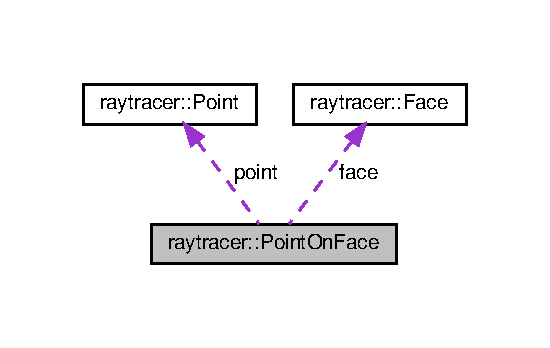
\includegraphics[width=264pt]{structraytracer_1_1PointOnFace__coll__graph}
\end{center}
\end{figure}
\subsection*{Public Attributes}
\begin{DoxyCompactItemize}
\item 
\mbox{\Hypertarget{structraytracer_1_1PointOnFace_a74a307612b3b86cabe4b1d5f618510e6}\label{structraytracer_1_1PointOnFace_a74a307612b3b86cabe4b1d5f618510e6}} 
\hyperlink{classraytracer_1_1Point}{Point} \hyperlink{structraytracer_1_1PointOnFace_a74a307612b3b86cabe4b1d5f618510e6}{point}
\begin{DoxyCompactList}\small\item\em The point. \end{DoxyCompactList}\item 
\mbox{\Hypertarget{structraytracer_1_1PointOnFace_afa20686364ca66cea1c3997d4d136cea}\label{structraytracer_1_1PointOnFace_afa20686364ca66cea1c3997d4d136cea}} 
const \hyperlink{classraytracer_1_1Face}{Face} $\ast$ \hyperlink{structraytracer_1_1PointOnFace_afa20686364ca66cea1c3997d4d136cea}{face}
\begin{DoxyCompactList}\small\item\em Pointer to the face the point is at. \end{DoxyCompactList}\end{DoxyCompactItemize}


\subsection{Detailed Description}
Structure representing a point on a face. 

This struct is used as return type of \hyperlink{namespaceraytracer_a82c9cab83ec5d18dca4be1b2cbde9dd2}{find\+Closest\+Intersection()}. 

The documentation for this struct was generated from the following file\+:\begin{DoxyCompactItemize}
\item 
/home/martin/\+C\+Lion\+Projects/raytracer/include/raytracer/geometry/Intersection.\+h\end{DoxyCompactItemize}

\hypertarget{classraytracer_1_1Ray}{}\section{raytracer\+:\+:Ray Class Reference}
\label{classraytracer_1_1Ray}\index{raytracer\+::\+Ray@{raytracer\+::\+Ray}}


Class representing a ray propagating through \hyperlink{classraytracer_1_1Mesh}{Mesh}.  




{\ttfamily \#include $<$Ray.\+h$>$}

\subsection*{Public Member Functions}
\begin{DoxyCompactItemize}
\item 
\hyperlink{classraytracer_1_1Ray_aa2a51f7caa322193c4b458ba960920f7}{Ray} (const \hyperlink{structraytracer_1_1HalfLine}{Half\+Line} \&initial\+Direction)
\begin{DoxyCompactList}\small\item\em Construct it using a \hyperlink{structraytracer_1_1HalfLine}{Half\+Line} (that is the initial direction of the \hyperlink{classraytracer_1_1Ray}{Ray}) \end{DoxyCompactList}\item 
{\footnotesize template$<$typename Direction\+Function , typename Intersection\+Function , typename Stop\+Condition $>$ }\\std\+::vector$<$ \hyperlink{structraytracer_1_1Intersection}{Intersection} $>$ \hyperlink{classraytracer_1_1Ray_a9ebcb3641ec730e5b94452833b69c68d}{find\+Intersections} (const \hyperlink{classraytracer_1_1Mesh}{Mesh} \&mesh, Direction\+Function find\+Direction, Intersection\+Function \hyperlink{namespaceraytracer_ae44c3032cf96db5f4ba9c07f12c9a207}{find\+Intersection}, Stop\+Condition stop\+Condition)
\begin{DoxyCompactList}\small\item\em Find intersections finds all the \hyperlink{structraytracer_1_1Intersection}{Intersection} with \hyperlink{classraytracer_1_1Mesh}{Mesh}. \end{DoxyCompactList}\end{DoxyCompactItemize}


\subsection{Detailed Description}
Class representing a ray propagating through \hyperlink{classraytracer_1_1Mesh}{Mesh}. 

Here the convention is such that the ray is made up of segments. These segments are given by std\+::vector of \hyperlink{structraytracer_1_1Intersection}{Intersection} with \hyperlink{classraytracer_1_1Mesh}{Mesh}. In general it is not a line and must not be straight. 

\subsection{Constructor \& Destructor Documentation}
\mbox{\Hypertarget{classraytracer_1_1Ray_aa2a51f7caa322193c4b458ba960920f7}\label{classraytracer_1_1Ray_aa2a51f7caa322193c4b458ba960920f7}} 
\index{raytracer\+::\+Ray@{raytracer\+::\+Ray}!Ray@{Ray}}
\index{Ray@{Ray}!raytracer\+::\+Ray@{raytracer\+::\+Ray}}
\subsubsection{\texorpdfstring{Ray()}{Ray()}}
{\footnotesize\ttfamily raytracer\+::\+Ray\+::\+Ray (\begin{DoxyParamCaption}\item[{const \hyperlink{structraytracer_1_1HalfLine}{Half\+Line} \&}]{initial\+Direction }\end{DoxyParamCaption})\hspace{0.3cm}{\ttfamily [inline]}, {\ttfamily [explicit]}}



Construct it using a \hyperlink{structraytracer_1_1HalfLine}{Half\+Line} (that is the initial direction of the \hyperlink{classraytracer_1_1Ray}{Ray}) 


\begin{DoxyParams}{Parameters}
{\em initial\+Direction} & \\
\hline
\end{DoxyParams}


\subsection{Member Function Documentation}
\mbox{\Hypertarget{classraytracer_1_1Ray_a9ebcb3641ec730e5b94452833b69c68d}\label{classraytracer_1_1Ray_a9ebcb3641ec730e5b94452833b69c68d}} 
\index{raytracer\+::\+Ray@{raytracer\+::\+Ray}!find\+Intersections@{find\+Intersections}}
\index{find\+Intersections@{find\+Intersections}!raytracer\+::\+Ray@{raytracer\+::\+Ray}}
\subsubsection{\texorpdfstring{find\+Intersections()}{findIntersections()}}
{\footnotesize\ttfamily template$<$typename Direction\+Function , typename Intersection\+Function , typename Stop\+Condition $>$ \\
std\+::vector$<$\hyperlink{structraytracer_1_1Intersection}{Intersection}$>$ raytracer\+::\+Ray\+::find\+Intersections (\begin{DoxyParamCaption}\item[{const \hyperlink{classraytracer_1_1Mesh}{Mesh} \&}]{mesh,  }\item[{Direction\+Function}]{find\+Direction,  }\item[{Intersection\+Function}]{find\+Intersection,  }\item[{Stop\+Condition}]{stop\+Condition }\end{DoxyParamCaption})\hspace{0.3cm}{\ttfamily [inline]}}



Find intersections finds all the \hyperlink{structraytracer_1_1Intersection}{Intersection} with \hyperlink{classraytracer_1_1Mesh}{Mesh}. 

There are multiple functional parameters to ensure high variability of this method.

\begin{DoxyNote}{Note}
{\bfseries This is the highly modular main method that does all the calculation.}
\end{DoxyNote}

\begin{DoxyTemplParams}{Template Parameters}
{\em Direction\+Function} & function type \\
\hline
{\em Intersection\+Function} & function type \\
\hline
{\em Stop\+Condition} & function type \\
\hline
\end{DoxyTemplParams}

\begin{DoxyParams}{Parameters}
{\em mesh} & to be intersected \\
\hline
{\em find\+Direction} & function that decides new direction every time a \hyperlink{classraytracer_1_1Face}{Face} is encountered. The function must have the following form\+: 
\begin{DoxyCode}
Vector findDirection()(
    \textcolor{keyword}{const} PointOnFace &pointOnFace,
    \textcolor{keyword}{const} Vector &previousDirection,
    \textcolor{keyword}{const} Element &previousElement,
    \textcolor{keyword}{const} Element &nextElement
) \{
    \textcolor{comment}{//x, y = ...}
    \textcolor{keywordflow}{return} Vector(x, y);
\}
\end{DoxyCode}
 It is recommended that you copy and paste this to implement find\+Direction. \\
\hline
{\em find\+Intersection} & function that finds the path of the \hyperlink{classraytracer_1_1Ray}{Ray} through given \hyperlink{classraytracer_1_1Element}{Element} and returns \hyperlink{structraytracer_1_1PointOnFace}{Point\+On\+Face} where the \hyperlink{classraytracer_1_1Ray}{Ray} escapes the \hyperlink{classraytracer_1_1Element}{Element}. The function mush have the following form\+: 
\begin{DoxyCode}
PointOnFace \hyperlink{namespaceraytracer_ae44c3032cf96db5f4ba9c07f12c9a207}{findIntersection}(
    \textcolor{keyword}{const} PointOnFace &entryPointOnFace,
    \textcolor{keyword}{const} Vector &entryDirection,
    \textcolor{keyword}{const} Element &element
) \{
    \textcolor{comment}{//point, face = ...}
    PointOnFace pointOnFace\{\};
    pointOnFace.point = point;
    pointOnFace.face = face;
    \textcolor{keywordflow}{return} pointOnFace;
\}
\end{DoxyCode}
 It is recommended that you copy and paste this to implement find\+Intersection. \\
\hline
{\em stop\+Condition} & function that returns true if the \hyperlink{classraytracer_1_1Ray}{Ray} should stop propagation. The function mush have the following form\+: 
\begin{DoxyCode}
\textcolor{keywordtype}{bool} stopCondition(
    \textcolor{keyword}{const} Element &
) \{
    \textcolor{comment}{//shouldStop = ...}
    \textcolor{keywordflow}{return} shouldStop;
\}
\end{DoxyCode}
 It is recommended that you copy and paste this to implement stop\+Condition. \\
\hline
\end{DoxyParams}
\begin{DoxyReturn}{Returns}

\end{DoxyReturn}


The documentation for this class was generated from the following file\+:\begin{DoxyCompactItemize}
\item 
/home/martin/\+C\+Lion\+Projects/raytracer/include/raytracer/geometry/Ray.\+h\end{DoxyCompactItemize}

\hypertarget{structraytracer_1_1SnellsLaw}{}\section{raytracer\+:\+:Snells\+Law Struct Reference}
\label{structraytracer_1_1SnellsLaw}\index{raytracer\+::\+Snells\+Law@{raytracer\+::\+Snells\+Law}}


Functor that finds new direction base on the Snells\textquotesingle{}s law.  




{\ttfamily \#include $<$Refraction.\+h$>$}

\subsection*{Public Member Functions}
\begin{DoxyCompactItemize}
\item 
\hyperlink{structraytracer_1_1SnellsLaw_a523a0d929eaaa78ea11bed701cac2d9d}{Snells\+Law} (const \hyperlink{classraytracer_1_1MeshFunction}{Mesh\+Function} \&density, const \hyperlink{classraytracer_1_1MeshFunction}{Mesh\+Function} \&temperature, const \hyperlink{classraytracer_1_1MeshFunction}{Mesh\+Function} \&ionization, const \hyperlink{classraytracer_1_1Gradient}{Gradient} \&gradient\+Calculator, const \hyperlink{classraytracer_1_1CollisionalFrequency}{Collisional\+Frequency} \&collisional\+Frequency\+Calculator)
\begin{DoxyCompactList}\small\item\em Construct the \hyperlink{structraytracer_1_1SnellsLaw}{Snells\+Law} using the density, temperature and ionization function references. \end{DoxyCompactList}\item 
\hyperlink{classraytracer_1_1Vector}{Vector} \hyperlink{structraytracer_1_1SnellsLaw_ab1af745f1e3b826546eff6d938b33982}{operator()} (const \hyperlink{structraytracer_1_1PointOnFace}{Point\+On\+Face} \&point\+On\+Face, const \hyperlink{classraytracer_1_1Vector}{Vector} \&previous\+Direction, const \hyperlink{classraytracer_1_1Element}{Element} \&previous\+Element, const \hyperlink{classraytracer_1_1Element}{Element} \&next\+Element, const \hyperlink{classraytracer_1_1LaserRay}{Laser\+Ray} \&laser\+Ray)
\begin{DoxyCompactList}\small\item\em Function to be used in \hyperlink{classraytracer_1_1Laser_a40fd2b112fb1de646861d7e93ac303e3}{Laser\+::generate\+Intersections()} as find\+Direction. \end{DoxyCompactList}\end{DoxyCompactItemize}


\subsection{Detailed Description}
Functor that finds new direction base on the Snells\textquotesingle{}s law. 

\subsection{Constructor \& Destructor Documentation}
\mbox{\Hypertarget{structraytracer_1_1SnellsLaw_a523a0d929eaaa78ea11bed701cac2d9d}\label{structraytracer_1_1SnellsLaw_a523a0d929eaaa78ea11bed701cac2d9d}} 
\index{raytracer\+::\+Snells\+Law@{raytracer\+::\+Snells\+Law}!Snells\+Law@{Snells\+Law}}
\index{Snells\+Law@{Snells\+Law}!raytracer\+::\+Snells\+Law@{raytracer\+::\+Snells\+Law}}
\subsubsection{\texorpdfstring{Snells\+Law()}{SnellsLaw()}}
{\footnotesize\ttfamily raytracer\+::\+Snells\+Law\+::\+Snells\+Law (\begin{DoxyParamCaption}\item[{const \hyperlink{classraytracer_1_1MeshFunction}{Mesh\+Function} \&}]{density,  }\item[{const \hyperlink{classraytracer_1_1MeshFunction}{Mesh\+Function} \&}]{temperature,  }\item[{const \hyperlink{classraytracer_1_1MeshFunction}{Mesh\+Function} \&}]{ionization,  }\item[{const \hyperlink{classraytracer_1_1Gradient}{Gradient} \&}]{gradient\+Calculator,  }\item[{const \hyperlink{classraytracer_1_1CollisionalFrequency}{Collisional\+Frequency} \&}]{collisional\+Frequency\+Calculator }\end{DoxyParamCaption})\hspace{0.3cm}{\ttfamily [explicit]}}



Construct the \hyperlink{structraytracer_1_1SnellsLaw}{Snells\+Law} using the density, temperature and ionization function references. 

Provide gradient\+Calculator calculate the plane of rarefaction. Provide collisional\+Frequency\+Calculator to evaluate the index of rarefaction. \hyperlink{structraytracer_1_1Density}{Density}, temperature and ionization values are expected to change. 
\begin{DoxyParams}{Parameters}
{\em density} & \\
\hline
{\em temperature} & \\
\hline
{\em ionization} & \\
\hline
{\em gradient\+Calculator} & \\
\hline
{\em collisional\+Frequency\+Calculator} & \\
\hline
\end{DoxyParams}


\subsection{Member Function Documentation}
\mbox{\Hypertarget{structraytracer_1_1SnellsLaw_ab1af745f1e3b826546eff6d938b33982}\label{structraytracer_1_1SnellsLaw_ab1af745f1e3b826546eff6d938b33982}} 
\index{raytracer\+::\+Snells\+Law@{raytracer\+::\+Snells\+Law}!operator()@{operator()}}
\index{operator()@{operator()}!raytracer\+::\+Snells\+Law@{raytracer\+::\+Snells\+Law}}
\subsubsection{\texorpdfstring{operator()()}{operator()()}}
{\footnotesize\ttfamily \hyperlink{classraytracer_1_1Vector}{Vector} raytracer\+::\+Snells\+Law\+::operator() (\begin{DoxyParamCaption}\item[{const \hyperlink{structraytracer_1_1PointOnFace}{Point\+On\+Face} \&}]{point\+On\+Face,  }\item[{const \hyperlink{classraytracer_1_1Vector}{Vector} \&}]{previous\+Direction,  }\item[{const \hyperlink{classraytracer_1_1Element}{Element} \&}]{previous\+Element,  }\item[{const \hyperlink{classraytracer_1_1Element}{Element} \&}]{next\+Element,  }\item[{const \hyperlink{classraytracer_1_1LaserRay}{Laser\+Ray} \&}]{laser\+Ray }\end{DoxyParamCaption})}



Function to be used in \hyperlink{classraytracer_1_1Laser_a40fd2b112fb1de646861d7e93ac303e3}{Laser\+::generate\+Intersections()} as find\+Direction. 

Finds new direction based on Snells law between the two \hyperlink{classraytracer_1_1Element}{Element}, density (provides an index of rarefaction) and gradient (provides edge direction). Could throw error no intersection found!


\begin{DoxyParams}{Parameters}
{\em point\+On\+Face} & \\
\hline
{\em previous\+Direction} & \\
\hline
{\em previous\+Element} & \\
\hline
{\em next\+Element} & \\
\hline
{\em laser\+Ray} & \\
\hline
\end{DoxyParams}
\begin{DoxyReturn}{Returns}
new direction based on Snells law. 
\end{DoxyReturn}


The documentation for this struct was generated from the following file\+:\begin{DoxyCompactItemize}
\item 
/home/martin/\+C\+Lion\+Projects/raytracer/include/raytracer/physics/Refraction.\+h\end{DoxyCompactItemize}

\hypertarget{classraytracer_1_1SpitzerFrequency}{}\section{raytracer\+:\+:Spitzer\+Frequency Class Reference}
\label{classraytracer_1_1SpitzerFrequency}\index{raytracer\+::\+Spitzer\+Frequency@{raytracer\+::\+Spitzer\+Frequency}}


Class representing a Spitzer-\/\+Harm frequency calculator.  




{\ttfamily \#include $<$Collisional\+Frequency.\+h$>$}



Inheritance diagram for raytracer\+:\+:Spitzer\+Frequency\+:
\nopagebreak
\begin{figure}[H]
\begin{center}
\leavevmode
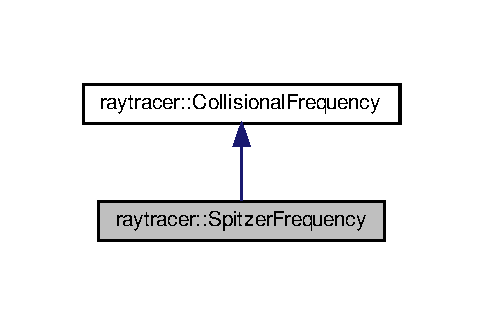
\includegraphics[width=232pt]{classraytracer_1_1SpitzerFrequency__inherit__graph}
\end{center}
\end{figure}


Collaboration diagram for raytracer\+:\+:Spitzer\+Frequency\+:
\nopagebreak
\begin{figure}[H]
\begin{center}
\leavevmode
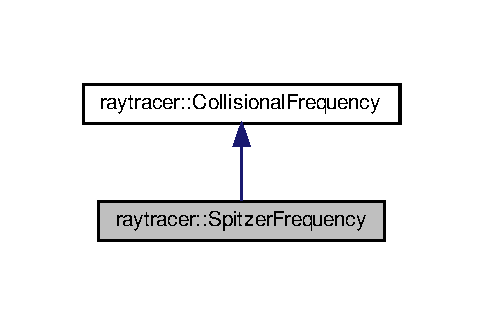
\includegraphics[width=232pt]{classraytracer_1_1SpitzerFrequency__coll__graph}
\end{center}
\end{figure}
\subsection*{Public Member Functions}
\begin{DoxyCompactItemize}
\item 
\hyperlink{structraytracer_1_1Frequency}{Frequency} \hyperlink{classraytracer_1_1SpitzerFrequency_aaead0d859dd82ad4ecc0a0805af954c5}{get} (const \hyperlink{structraytracer_1_1Density}{Density} \&density, const \hyperlink{structraytracer_1_1Temperature}{Temperature} \&temperature, const \hyperlink{structraytracer_1_1Length}{Length} \&laser\+Wavelength, double ionization) const override
\begin{DoxyCompactList}\small\item\em Based on the state variables return the Spitzer Harm frequency obtained according to Velechovsky thesis. \end{DoxyCompactList}\end{DoxyCompactItemize}


\subsection{Detailed Description}
Class representing a Spitzer-\/\+Harm frequency calculator. 

\subsection{Member Function Documentation}
\mbox{\Hypertarget{classraytracer_1_1SpitzerFrequency_aaead0d859dd82ad4ecc0a0805af954c5}\label{classraytracer_1_1SpitzerFrequency_aaead0d859dd82ad4ecc0a0805af954c5}} 
\index{raytracer\+::\+Spitzer\+Frequency@{raytracer\+::\+Spitzer\+Frequency}!get@{get}}
\index{get@{get}!raytracer\+::\+Spitzer\+Frequency@{raytracer\+::\+Spitzer\+Frequency}}
\subsubsection{\texorpdfstring{get()}{get()}}
{\footnotesize\ttfamily \hyperlink{structraytracer_1_1Frequency}{Frequency} raytracer\+::\+Spitzer\+Frequency\+::get (\begin{DoxyParamCaption}\item[{const \hyperlink{structraytracer_1_1Density}{Density} \&}]{density,  }\item[{const \hyperlink{structraytracer_1_1Temperature}{Temperature} \&}]{temperature,  }\item[{const \hyperlink{structraytracer_1_1Length}{Length} \&}]{laser\+Wavelength,  }\item[{double}]{ionization }\end{DoxyParamCaption}) const\hspace{0.3cm}{\ttfamily [override]}, {\ttfamily [virtual]}}



Based on the state variables return the Spitzer Harm frequency obtained according to Velechovsky thesis. 


\begin{DoxyParams}{Parameters}
{\em density} & \\
\hline
{\em temperature} & \\
\hline
{\em laser\+Wavelength} & \\
\hline
{\em ionization} & \\
\hline
\end{DoxyParams}
\begin{DoxyReturn}{Returns}
the collisional frequency 
\end{DoxyReturn}


Implements \hyperlink{classraytracer_1_1CollisionalFrequency_a85c4e6175a8a692e02be34cdccbf1e16}{raytracer\+::\+Collisional\+Frequency}.



The documentation for this class was generated from the following file\+:\begin{DoxyCompactItemize}
\item 
/home/martin/\+C\+Lion\+Projects/raytracer/include/raytracer/physics/Collisional\+Frequency.\+h\end{DoxyCompactItemize}

\hypertarget{classraytracer_1_1StepGradient}{}\section{raytracer\+:\+:Step\+Gradient Class Reference}
\label{classraytracer_1_1StepGradient}\index{raytracer\+::\+Step\+Gradient@{raytracer\+::\+Step\+Gradient}}


Gradient\+Calculator that returns the normal to the face as \hyperlink{classraytracer_1_1Gradient}{Gradient}.  




{\ttfamily \#include $<$Gradient.\+h$>$}



Inheritance diagram for raytracer\+:\+:Step\+Gradient\+:
\nopagebreak
\begin{figure}[H]
\begin{center}
\leavevmode
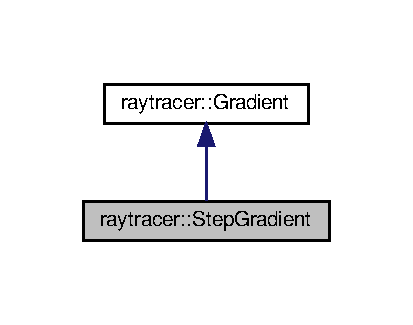
\includegraphics[width=198pt]{classraytracer_1_1StepGradient__inherit__graph}
\end{center}
\end{figure}


Collaboration diagram for raytracer\+:\+:Step\+Gradient\+:
\nopagebreak
\begin{figure}[H]
\begin{center}
\leavevmode
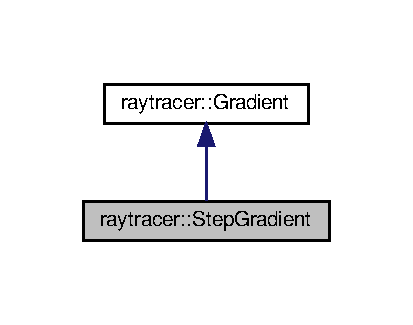
\includegraphics[width=198pt]{classraytracer_1_1StepGradient__coll__graph}
\end{center}
\end{figure}
\subsection*{Public Member Functions}
\begin{DoxyCompactItemize}
\item 
\hyperlink{classraytracer_1_1Vector}{Vector} \hyperlink{classraytracer_1_1StepGradient_a0c18f1abff911e8ebd91184b55c8c0ef}{get} (const \hyperlink{structraytracer_1_1PointOnFace}{Point\+On\+Face} \&point\+On\+Face, const \hyperlink{classraytracer_1_1Element}{Element} \&, const \hyperlink{classraytracer_1_1Element}{Element} \&) const override
\begin{DoxyCompactList}\small\item\em Get gradient as a normal to the \hyperlink{classraytracer_1_1Face}{Face} given by \hyperlink{structraytracer_1_1PointOnFace}{Point\+On\+Face}. \end{DoxyCompactList}\end{DoxyCompactItemize}


\subsection{Detailed Description}
Gradient\+Calculator that returns the normal to the face as \hyperlink{classraytracer_1_1Gradient}{Gradient}. 

\subsection{Member Function Documentation}
\mbox{\Hypertarget{classraytracer_1_1StepGradient_a0c18f1abff911e8ebd91184b55c8c0ef}\label{classraytracer_1_1StepGradient_a0c18f1abff911e8ebd91184b55c8c0ef}} 
\index{raytracer\+::\+Step\+Gradient@{raytracer\+::\+Step\+Gradient}!get@{get}}
\index{get@{get}!raytracer\+::\+Step\+Gradient@{raytracer\+::\+Step\+Gradient}}
\subsubsection{\texorpdfstring{get()}{get()}}
{\footnotesize\ttfamily \hyperlink{classraytracer_1_1Vector}{Vector} raytracer\+::\+Step\+Gradient\+::get (\begin{DoxyParamCaption}\item[{const \hyperlink{structraytracer_1_1PointOnFace}{Point\+On\+Face} \&}]{point\+On\+Face,  }\item[{const \hyperlink{classraytracer_1_1Element}{Element} \&}]{,  }\item[{const \hyperlink{classraytracer_1_1Element}{Element} \&}]{ }\end{DoxyParamCaption}) const\hspace{0.3cm}{\ttfamily [inline]}, {\ttfamily [override]}, {\ttfamily [virtual]}}



Get gradient as a normal to the \hyperlink{classraytracer_1_1Face}{Face} given by \hyperlink{structraytracer_1_1PointOnFace}{Point\+On\+Face}. 


\begin{DoxyParams}{Parameters}
{\em point\+On\+Face} & \\
\hline
\end{DoxyParams}
\begin{DoxyReturn}{Returns}
normal as gradient 
\end{DoxyReturn}


Implements \hyperlink{classraytracer_1_1Gradient_a93ccfef0662634c5f9a3c8dd04e73496}{raytracer\+::\+Gradient}.



The documentation for this class was generated from the following file\+:\begin{DoxyCompactItemize}
\item 
/home/martin/\+C\+Lion\+Projects/raytracer/include/raytracer/physics/Gradient.\+h\end{DoxyCompactItemize}

\hypertarget{structraytracer_1_1StopAtCritical}{}\section{raytracer\+:\+:Stop\+At\+Critical Struct Reference}
\label{structraytracer_1_1StopAtCritical}\index{raytracer\+::\+Stop\+At\+Critical@{raytracer\+::\+Stop\+At\+Critical}}


Functor for ray propagation termination based on critical density expected to used with lase\+Ray intersection finding procedure.  




{\ttfamily \#include $<$Termination.\+h$>$}

\subsection*{Public Member Functions}
\begin{DoxyCompactItemize}
\item 
\hyperlink{structraytracer_1_1StopAtCritical_a61743eacd97c1af03146aa64aa9c95e5}{Stop\+At\+Critical} (const \hyperlink{classraytracer_1_1MeshFunction}{Mesh\+Function} \&density)
\begin{DoxyCompactList}\small\item\em Constructor the functor using a density \hyperlink{classraytracer_1_1MeshFunction}{Mesh\+Function}. \end{DoxyCompactList}\item 
bool \hyperlink{structraytracer_1_1StopAtCritical_acc71054d773ea6fe0df52986d5d1512e}{operator()} (const \hyperlink{classraytracer_1_1Element}{Element} \&element, const \hyperlink{classraytracer_1_1LaserRay}{Laser\+Ray} \&laser\+Ray)
\begin{DoxyCompactList}\small\item\em Returns true if the density at element to go to is greater than critical\+Density of the \hyperlink{classraytracer_1_1LaserRay}{Laser\+Ray}. \end{DoxyCompactList}\end{DoxyCompactItemize}


\subsection{Detailed Description}
Functor for ray propagation termination based on critical density expected to used with lase\+Ray intersection finding procedure. 

\subsection{Constructor \& Destructor Documentation}
\mbox{\Hypertarget{structraytracer_1_1StopAtCritical_a61743eacd97c1af03146aa64aa9c95e5}\label{structraytracer_1_1StopAtCritical_a61743eacd97c1af03146aa64aa9c95e5}} 
\index{raytracer\+::\+Stop\+At\+Critical@{raytracer\+::\+Stop\+At\+Critical}!Stop\+At\+Critical@{Stop\+At\+Critical}}
\index{Stop\+At\+Critical@{Stop\+At\+Critical}!raytracer\+::\+Stop\+At\+Critical@{raytracer\+::\+Stop\+At\+Critical}}
\subsubsection{\texorpdfstring{Stop\+At\+Critical()}{StopAtCritical()}}
{\footnotesize\ttfamily raytracer\+::\+Stop\+At\+Critical\+::\+Stop\+At\+Critical (\begin{DoxyParamCaption}\item[{const \hyperlink{classraytracer_1_1MeshFunction}{Mesh\+Function} \&}]{density }\end{DoxyParamCaption})\hspace{0.3cm}{\ttfamily [explicit]}}



Constructor the functor using a density \hyperlink{classraytracer_1_1MeshFunction}{Mesh\+Function}. 


\begin{DoxyParams}{Parameters}
{\em density} & \\
\hline
\end{DoxyParams}


\subsection{Member Function Documentation}
\mbox{\Hypertarget{structraytracer_1_1StopAtCritical_acc71054d773ea6fe0df52986d5d1512e}\label{structraytracer_1_1StopAtCritical_acc71054d773ea6fe0df52986d5d1512e}} 
\index{raytracer\+::\+Stop\+At\+Critical@{raytracer\+::\+Stop\+At\+Critical}!operator()@{operator()}}
\index{operator()@{operator()}!raytracer\+::\+Stop\+At\+Critical@{raytracer\+::\+Stop\+At\+Critical}}
\subsubsection{\texorpdfstring{operator()()}{operator()()}}
{\footnotesize\ttfamily bool raytracer\+::\+Stop\+At\+Critical\+::operator() (\begin{DoxyParamCaption}\item[{const \hyperlink{classraytracer_1_1Element}{Element} \&}]{element,  }\item[{const \hyperlink{classraytracer_1_1LaserRay}{Laser\+Ray} \&}]{laser\+Ray }\end{DoxyParamCaption})}



Returns true if the density at element to go to is greater than critical\+Density of the \hyperlink{classraytracer_1_1LaserRay}{Laser\+Ray}. 


\begin{DoxyParams}{Parameters}
{\em element} & \\
\hline
{\em laser\+Ray} & \\
\hline
\end{DoxyParams}
\begin{DoxyReturn}{Returns}
true if current density is grater than critical 
\end{DoxyReturn}


The documentation for this struct was generated from the following file\+:\begin{DoxyCompactItemize}
\item 
/home/martin/\+C\+Lion\+Projects/raytracer/include/raytracer/physics/Termination.\+h\end{DoxyCompactItemize}

\hypertarget{structraytracer_1_1Temperature}{}\section{raytracer\+:\+:Temperature Struct Reference}
\label{structraytracer_1_1Temperature}\index{raytracer\+::\+Temperature@{raytracer\+::\+Temperature}}


Strong type representing temperature in eV.  




{\ttfamily \#include $<$Magnitudes.\+h$>$}



\subsection{Detailed Description}
Strong type representing temperature in eV. 



The documentation for this struct was generated from the following file\+:\begin{DoxyCompactItemize}
\item 
/home/martin/\+C\+Lion\+Projects/raytracer/include/raytracer/physics/Magnitudes.\+h\end{DoxyCompactItemize}

\hypertarget{classraytracer_1_1Vector}{}\section{raytracer\+:\+:Vector Class Reference}
\label{classraytracer_1_1Vector}\index{raytracer\+::\+Vector@{raytracer\+::\+Vector}}


Class representing a physical vector.  




{\ttfamily \#include $<$Vector.\+h$>$}

\subsection*{Public Member Functions}
\begin{DoxyCompactItemize}
\item 
\hyperlink{classraytracer_1_1Vector_a4a257f16b43edb428655be54c640fb69}{Vector} (double \hyperlink{classraytracer_1_1Vector_a14aa5241f6abb01266ea77586fa1437a}{x}, double \hyperlink{classraytracer_1_1Vector_ad4d58fd3af1dbf59eae8c55a67e85b3a}{y})
\begin{DoxyCompactList}\small\item\em Construct the vector using its coordinates. \end{DoxyCompactList}\item 
\mbox{\Hypertarget{classraytracer_1_1Vector_ab6d9a3c5c8d49c49376b11bbfa2d64ae}\label{classraytracer_1_1Vector_ab6d9a3c5c8d49c49376b11bbfa2d64ae}} 
\hyperlink{classraytracer_1_1Vector_ab6d9a3c5c8d49c49376b11bbfa2d64ae}{Vector} ()=default
\begin{DoxyCompactList}\small\item\em Default constructor initializes a (0, 0) vector. \end{DoxyCompactList}\item 
double \hyperlink{classraytracer_1_1Vector_a33106a20cb1d9c921664a7622c41cf6b}{get\+Norm} () const
\begin{DoxyCompactList}\small\item\em Return the Euclidean norm of the vector (square root of sum of coordinates squared) \end{DoxyCompactList}\item 
\hyperlink{classraytracer_1_1Vector}{Vector} \hyperlink{classraytracer_1_1Vector_a21d2e5fd46c25b7e1c33fec1ecc9bd95}{get\+Normal} () const
\begin{DoxyCompactList}\small\item\em Return the normal to the vector using the convention (y, -\/x) \end{DoxyCompactList}\end{DoxyCompactItemize}
\subsection*{Public Attributes}
\begin{DoxyCompactItemize}
\item 
\mbox{\Hypertarget{classraytracer_1_1Vector_a14aa5241f6abb01266ea77586fa1437a}\label{classraytracer_1_1Vector_a14aa5241f6abb01266ea77586fa1437a}} 
double \hyperlink{classraytracer_1_1Vector_a14aa5241f6abb01266ea77586fa1437a}{x}
\begin{DoxyCompactList}\small\item\em x coordinate \end{DoxyCompactList}\item 
\mbox{\Hypertarget{classraytracer_1_1Vector_ad4d58fd3af1dbf59eae8c55a67e85b3a}\label{classraytracer_1_1Vector_ad4d58fd3af1dbf59eae8c55a67e85b3a}} 
double \hyperlink{classraytracer_1_1Vector_ad4d58fd3af1dbf59eae8c55a67e85b3a}{y}
\begin{DoxyCompactList}\small\item\em y coordinate \end{DoxyCompactList}\end{DoxyCompactItemize}


\subsection{Detailed Description}
Class representing a physical vector. 

\subsection{Constructor \& Destructor Documentation}
\mbox{\Hypertarget{classraytracer_1_1Vector_a4a257f16b43edb428655be54c640fb69}\label{classraytracer_1_1Vector_a4a257f16b43edb428655be54c640fb69}} 
\index{raytracer\+::\+Vector@{raytracer\+::\+Vector}!Vector@{Vector}}
\index{Vector@{Vector}!raytracer\+::\+Vector@{raytracer\+::\+Vector}}
\subsubsection{\texorpdfstring{Vector()}{Vector()}}
{\footnotesize\ttfamily raytracer\+::\+Vector\+::\+Vector (\begin{DoxyParamCaption}\item[{double}]{x,  }\item[{double}]{y }\end{DoxyParamCaption})}



Construct the vector using its coordinates. 


\begin{DoxyParams}{Parameters}
{\em x} & coordinate \\
\hline
{\em y} & coordinate \\
\hline
\end{DoxyParams}


\subsection{Member Function Documentation}
\mbox{\Hypertarget{classraytracer_1_1Vector_a33106a20cb1d9c921664a7622c41cf6b}\label{classraytracer_1_1Vector_a33106a20cb1d9c921664a7622c41cf6b}} 
\index{raytracer\+::\+Vector@{raytracer\+::\+Vector}!get\+Norm@{get\+Norm}}
\index{get\+Norm@{get\+Norm}!raytracer\+::\+Vector@{raytracer\+::\+Vector}}
\subsubsection{\texorpdfstring{get\+Norm()}{getNorm()}}
{\footnotesize\ttfamily double raytracer\+::\+Vector\+::get\+Norm (\begin{DoxyParamCaption}{ }\end{DoxyParamCaption}) const}



Return the Euclidean norm of the vector (square root of sum of coordinates squared) 

\begin{DoxyReturn}{Returns}
size of the vector 
\end{DoxyReturn}
\mbox{\Hypertarget{classraytracer_1_1Vector_a21d2e5fd46c25b7e1c33fec1ecc9bd95}\label{classraytracer_1_1Vector_a21d2e5fd46c25b7e1c33fec1ecc9bd95}} 
\index{raytracer\+::\+Vector@{raytracer\+::\+Vector}!get\+Normal@{get\+Normal}}
\index{get\+Normal@{get\+Normal}!raytracer\+::\+Vector@{raytracer\+::\+Vector}}
\subsubsection{\texorpdfstring{get\+Normal()}{getNormal()}}
{\footnotesize\ttfamily \hyperlink{classraytracer_1_1Vector}{Vector} raytracer\+::\+Vector\+::get\+Normal (\begin{DoxyParamCaption}{ }\end{DoxyParamCaption}) const\hspace{0.3cm}{\ttfamily [inline]}}



Return the normal to the vector using the convention (y, -\/x) 

\begin{DoxyReturn}{Returns}

\end{DoxyReturn}


The documentation for this class was generated from the following file\+:\begin{DoxyCompactItemize}
\item 
/home/martin/\+C\+Lion\+Projects/raytracer/include/raytracer/geometry/Vector.\+h\end{DoxyCompactItemize}

%--- End generated contents ---

% Index
\backmatter
\newpage
\phantomsection
\clearemptydoublepage
\addcontentsline{toc}{chapter}{Index}
\printindex

\end{document}
